% Document class definition
\documentclass[final,a4paper,11pt,twoside]{class_diss}

% Package imports
% Basic packages
\usepackage[utf8]{inputenc}
\usepackage[T1]{fontenc}
\usepackage[spanish,es-tabla]{babel}
\usepackage[margin=3cm]{geometry}
\usepackage{setspace}
\usepackage{url}
\usepackage{xspace}

% Math packages
\usepackage{amsmath}
\usepackage{amsxtra}
\usepackage{amssymb}
\usepackage{amsthm}
\usepackage{latexsym}
\usepackage{bbold}
\usepackage{stmaryrd}

% Graphics packages
\usepackage{graphicx}
\usepackage[svgnames,dvipsnames,table,xcdraw]{xcolor}
\usepackage{tikz}
\usetikzlibrary{shapes}

% Table packages
\usepackage{booktabs}
\usepackage{multirow}

% List and enumeration packages
\usepackage{enumitem}

% Floating object packages
\usepackage{float}
\usepackage{rotating}
\usepackage{pdflscape}
\usepackage{placeins}
\usepackage{flafter}

% Code listing packages
\usepackage{listings}

% Algorithm packages
\usepackage[ruled,vlined]{algorithm2e}
\usepackage{algorithmic}

% Bibliography and citation packages
\usepackage[authoryear,sort&compress]{natbib}
\usepackage{hypernat}
\bibliographystyle{apa}
\setcitestyle{authoryear}

% Glossary packages
\usepackage[pdftex,plainpages=false,pdfpagelabels]{hyperref}\usepackage[toc,acronym,nonumberlist,xindy={language=spanish-traditional},sanitize=none]{glossaries}

\makeglossaries

% Formatting packages
\usepackage[full]{textcomp}
\usepackage[scaled]{helvet}
\usepackage[titles]{tocloft}
\usepackage[explicit]{titlesec}
\usepackage{emptypage}
\usepackage{soul}
\usepackage[colorinlistoftodos, textwidth=2.5cm]{todonotes}
\usepackage{fancyhdr}


% Custom commands and settings
\theoremstyle{definition}
\newtheorem{definition}{Teorema}[section]
\theoremstyle{remark}
\newtheorem*{remark}{Remark}
\DeclareMathOperator*{\argmax}{arg\,max}
\DeclareMathOperator*{\argmin}{arg\,min}

% Color definitions
\definecolor{VIU}{RGB}{240, 90, 15}
\definecolor{DESTACADO}{RGB}{130, 34, 145}
\definecolor{CITA}{RGB}{0, 123, 194}

% Custom commands
\renewcommand{\algorithmcfname}{Algoritmo}
\renewcommand{\acronymname}{Lista de Acrónimos}
\addto\captionsspanish{
    \renewcommand*{\acronymname}{Lista de Acrónimos}
}
\newcommand{\inhib}{\relbar\mapsfromchar}
\newcommand{\destacado}[1]{\color{DESTACADO}\textbf{#1}\color{black}\xspace}
\newcommand*\circled[1]{\tikz[baseline=(char.base)]{
    \node[shape=diamond,fill=black!90,inner sep=1pt,minimum size=1cm] (char) {\textcolor{white}{\small\textbf{#1}}};}
}

% Fancyhdr settings
\setlength{\headheight}{14pt}
\pagestyle{fancy}
\fancyhf{}
\fancyhead[LO]{}
\fancyhead[RE]{}
\fancyfoot[C]{}
\renewcommand{\headrulewidth}{0pt}

\fancypagestyle{plain}{
  \fancyhf{}
  \fancyfoot[C]{\circled{\thepage}}
  \renewcommand{\headrulewidth}{0pt}
}

% Chapter title formatting
\colorlet{chapnumcolor}{VIU}
\newcommand*{\chapnumfont}{%
  \usefont{T1}{jkp}{b}{n}%
  \fontsize{70}{90}%
  \selectfont%
}
\newcommand*{\chaptitlefont}{%
  \usefont{T1}{qhv}{b}{n}%
  \fontsize{22}{26}%
  \selectfont%
}
\titleformat{name=\chapter}
{\normalfont\huge\bfseries}
{\rlap{\parbox{\textwidth}{\filleft\chapnumfont\color{chapnumcolor}\thechapter}}}
{0pt}
{\rlap{\parbox{0.7\textwidth}{\filright\chaptitlefont #1}}}

% Glossary entries
% Glosario

% Estado del arte
\newglossaryentry{rl}{
  name={RL},
  description={Reinforcement Learning - Aprendizaje por Refuerzo, una rama de la IA que permite a los sistemas aprender a través de la interacción con un entorno},
  first={Reinforcement Learning (RL)\glsadd{rl}}
}

\newglossaryentry{multi-agent}{
  name={Sistema Multi-Agente},
  description={Sistema compuesto por múltiples agentes inteligentes que interactúan entre sí para resolver problemas complejos},
  first={Sistema Multi-Agente\glsadd{multi-agent}}
}

\newglossaryentry{data-mining}{
  name={Data Mining},
  description={Proceso de descubrir patrones y relaciones en grandes conjuntos de datos},
  first={Data Mining\glsadd{data-mining}}
}

\newglossaryentry{agentic-ia}{
  name={IA Agéntica},
  description={Un tipo de inteligencia artificial que actúa de manera autónoma y proactiva, tomando decisiones y realizando acciones para alcanzar objetivos específicos}
}

\newglossaryentry{open-source}{
  name={Código Abierto},
  description={Software cuyo código fuente está disponible públicamente y puede ser modificado y distribuido por cualquier persona}
}

\newglossaryentry{sla}{
  name={SLA},
  description={Second Language Acquisition - Proceso de adquisición de una segunda lengua},
  first={Second Language Acquisition (SLA)\glsadd{sla}}
}

\newglossaryentry{input}{
  name={Input Hypothesis},
  description={Hipótesis propuesta por Krashen que establece que los aprendices progresan cuando reciben input comprensible},
  first={Input Hypothesis\glsadd{input}}
}

\newglossaryentry{ia}{
  name={IA},
  description={Inteligencia Artificial - Conjunto de tecnologías que permiten a las máquinas aprender, razonar y tomar decisiones},
  first={Inteligencia Artificial (IA)\glsadd{ia}}
}

\newglossaryentry{transformers}{
  name={Transformers},
  description={Arquitectura de red neuronal que ha revolucionado el procesamiento del lenguaje natural},
  first={Transformers\glsadd{transformers}}
}

\newglossaryentry{tts}{
  name=TTS,
  description={Text-to-Speech (Texto a Voz). Sistema que convierte texto escrito en habla sintetizada},
  first={Text-to-Speech (TTS)\glsadd{tts}},
  long={Text-to-Speech}
}

\newglossaryentry{stt}{
  name=STT,
  description={Speech-to-Text (Voz a Texto). Sistema que convierte el habla en texto escrito mediante reconocimiento automático del habla},
  first={Speech-to-Text (STT)\glsadd{stt}},
  long={Speech-to-Text}
}

\newglossaryentry{rag}{
  name={RAG},
  description={Retrieval-Augmented Generation - Sistema que combina la recuperación de información con la generación de texto},
  first={Retrieval-Augmented Generation (RAG)\glsadd{rag}}
}

\newglossaryentry{llm}{
  name={LLM},
  description={Large Language Model - Modelo de lenguaje de gran escala},
  first={Large Language Model (LLM)\glsadd{llm}}
}

\newglossaryentry{nlp}{
  name={NLP},
  description={Natural Language Processing - Procesamiento del Lenguaje Natural},
  first={Natural Language Processing (NLP)\glsadd{nlp}}
}

\newglossaryentry{tensorflow}{
  name={TensorFlow},
  description={Biblioteca de código abierto para aprendizaje automático desarrollada por Google},
  first={TensorFlow\glsadd{tensorflow}}
}

\newglossaryentry{py-torch}{
  name={PyTorch},
  description={Biblioteca de aprendizaje profundo de código abierto desarrollada por Meta},
  first={PyTorch\glsadd{py-torch}}
}

% Marco teórico
\newglossaryentry{its}{
  name={ITS},
  description={Intelligent Tutoring System - Sistema de Tutoría Inteligente},
  first={Intelligent Tutoring System (ITS)\glsadd{its}}
}

\newglossaryentry{adaptive}{
  name={Sistema Adaptativo},
  description={Sistema capaz de modificar su comportamiento según las necesidades del usuario},
  first={Sistema Adaptativo\glsadd{adaptive}}
}

\newglossaryentry{recommender}{
  name={Sistema de Recomendación},
  description={Sistema que sugiere contenido relevante basado en el perfil del usuario y su comportamiento},
  first={Sistema de Recomendación\glsadd{recommender}}
}

\newglossaryentry{attention}{
  name={Mecanismo de Atención},
  description={Componente clave de la arquitectura Transformer que permite al modelo enfocarse en diferentes partes de la entrada según su relevancia},
  first={Mecanismo de Atención\glsadd{attention}}
}

\newglossaryentry{feed-forward}{
  name={Feed-Forward},
  description={Capa de red neuronal que aplica una transformación lineal seguida de una función de activación},
  first={Feed-Forward\glsadd{feed-forward}}
}

\newglossaryentry{self-attention}{
  name={Auto-Atención},
  description={Mecanismo que permite a un modelo evaluar las relaciones entre todas las posiciones de una secuencia},
  first={Auto-Atención\glsadd{self-attention}}
}

\newglossaryentry{token}{
  name={Token},
  description={Unidad básica de procesamiento en modelos de lenguaje, que puede ser una palabra, subpalabra o carácter},
  first={Token\glsadd{token}}
}

\newglossaryentry{perplexity}{
  name={Perplejidad},
  description={Métrica que evalúa qué tan bien un modelo de lenguaje predice una muestra de texto},
  first={Perplejidad\glsadd{perplexity}}
}

\newglossaryentry{retriever}{
  name={Recuperador},
  description={Componente de un sistema de recuperación de información que selecciona documentos relevantes a partir de una consulta},
  first={Recuperador\glsadd{retriever}}
}

\newglossaryentry{generator}{
  name={Generador},
  description={Componente de un sistema de recuperación de información que crea respuestas a partir de los documentos recuperados},
  first={Generador\glsadd{generator}}
}

\newglossaryentry{hallucinations}{
  name={Alucinaciones},
  description={Errores en la generación de texto que resultan en respuestas incoherentes o incorrectas},
  first={Alucinaciones\glsadd{hallucinations}}
}

\newglossaryentry{mdp}{
  name={MDP},
  description={Markov Decision Process - Marco matemático para modelar la toma de decisiones en situaciones donde los resultados son parcialmente aleatorios y parcialmente bajo control},
  first={Markov Decision Process (MDP)\glsadd{mdp}}
}

\newglossaryentry{policy}{
  name={Política},
  description={Estrategia que sigue un agente para determinar sus acciones basándose en el estado actual del estudiante},
  first={Política\glsadd{policy}}
}

\newglossaryentry{reward-function}{
  name={Función de Recompensa},
  description={Función que define la retroalimentación que recibe el agente basada en el progreso del estudiante},
  first={Función de Recompensa\glsadd{reward-function}}
}

\newglossaryentry{reward}{
  name={Recompensa},
  description={Valor numérico que indica el éxito o fracaso de una acción tomada por el agente},
  first={Recompensa\glsadd{reward}}
}

\newglossaryentry{engagement}{
  name={Compromiso},
  description={Indicador de la motivación y el interés del estudiante en la tarea de aprendizaje},
  first={Compromiso\glsadd{engagement}}
}

\newglossaryentry{exploitation}{
  name={Explotación},
  description={Estrategia de selección de acciones que se basa en la información ya conocida para maximizar la recompensa},
  first={Explotación\glsadd{exploitation}}
}

\newglossaryentry{exploration}{
  name={Exploración},
  description={Estrategia de selección de acciones que busca descubrir nuevas opciones y mejorar el conocimiento del agente},
  first={Exploración\glsadd{exploration}}
}

\newglossaryentry{knowledge-base}{
  name={Base de Conocimiento},
  description={Conjunto de datos estructurados que almacena información relevante para un sistema de recuperación de información},
  first={Base de Conocimiento\glsadd{knowledge-base}}
}

\newglossaryentry{whisper}{
  name=Whisper,
  description={Modelo de reconocimiento de voz de código abierto desarrollado por OpenAI, capaz de realizar transcripción y traducción en múltiples idiomas},
  first={Whisper\glsadd{whisper}}
}

\newglossaryentry{coqui}{
  name=Coqui TTS,
  description={Suite de herramientas open source para síntesis de voz que incluye múltiples arquitecturas y modelos pre-entrenados},
  first={Coqui TTS\glsadd{coqui}}
}

\newglossaryentry{mfcc}{
  name=MFCC,
  description={Mel-Frequency Cepstral Coefficients. Coeficientes que representan el espectro de potencia a corto plazo de un sonido, basados en una transformación coseno lineal de un espectro de potencia logarítmico en una escala de frecuencia mel no lineal},
  first={Mel-Frequency Cepstral Coefficients (MFCC)\glsadd{mfcc}}
}

\newglossaryentry{viterbi}{
  name=Viterbi,
  description={Algoritmo que encuentra la secuencia más probable de estados ocultos en un modelo oculto de Markov, comúnmente usado en reconocimiento de voz para decodificación},
  first={Viterbi\glsadd{viterbi}}
}

\newglossaryentry{beam-search}{
  name=Beam Search,
  description={Algoritmo de búsqueda heurística que explora un grafo construyendo el grafo gradualmente desde la raíz, expandiendo el nodo más prometedor en un conjunto limitado de nodos},
  first={Beam Search\glsadd{beam-search}}
}

% Acrónimos
\newacronym{bert}{BERT}{Bidirectional Encoder Representations from Transformers}
\newacronym{gan}{GAN}{Generative Adversarial Network}


% Hyperref settings
\hypersetup{
    linktocpage=true,
    colorlinks=true,
    citecolor=CITA,
    urlcolor=CITA,
    linkcolor=CITA,
    citebordercolor={1 0 0},
    urlbordercolor={1 0 0},
    linkbordercolor={.7 .8 .8},
    breaklinks=true,
}

% Document settings
\setcounter{secnumdepth}{3}
\onehalfspacing
\renewcommand\familydefault{\sfdefault}

% Begin document
\begin{document}

\pagestyle{empty}
\begin{titlepage}
  \begin{center}
    \includegraphics[width=0.60\textwidth]{figuras/viu.png} \\[1cm]

    \huge \textbf{Aplicación de Reinforcement Learning y Transformers para el Aprendizaje de Idiomas} \\[1cm]

    \large Trabajo Fin de Máster, \\
    \large Convocatoria Marzo 2025 \\

    \vspace{2cm}

    \Large \textbf{Máster Propio en Inteligencia Artificial} \\[0.5cm]
    \large Segunda Edición, \\
    \large Curso Académico 2024 \\

    \vspace{2cm}

    \large Por el alumno/a \\
    \Large \textbf{Julio Emanuel Suriano Bryk} \\
    \large Con DNI 37.620.411 \\[1cm]

    \vspace{1cm}

    \large Dirigido por \\
    \Large \textbf{José Gabriel García Pardo} \\
  \end{center}
\end{titlepage}
\cleardoublepage

\null\vspace{\stretch{2}}
{
    \hfill \begin{minipage}{10cm}
        \textsl{
            \begin{flushright}
                Education is not about thinning the herd.\\
                Education is about helping every student succeed.
            \end{flushright}
        }

        \begin{flushright}
            Andrew Ng
        \end{flushright}

    \end{minipage}
}
\vspace{\stretch{1}}

\cleardoublepage
\normalfont{\huge{\bfseries{Agradecimientos}}}
\vspace{15ex}

Me gustaría agradecer a los profesores y compañeros del máster por su apoyo, sus valiosas aportaciones y los intercambios de ideas que han enriquecido este trabajo.

\medskip
También quiero destacar a mi pareja por su comprensión y apoyo durante todo el proceso, lo que me permitió mantenerme enfocado y motivado.

\medskip
Por último, agradezco a mi familia y amigos por su apoyo constante y por estar siempre disponibles para ofrecerme su ayuda y perspectiva.


\pagestyle{fancy}

\newpage

\renewcommand{\headrulewidth}{0.4pt}

\pdfbookmark[0]{\contentsname}{contents}

\renewcommand{\cftchapleader}{\cftdotfill{\cftdotsep}}
\renewcommand{\cftchapfont}{\mdseries}
\renewcommand{\cftchappagefont}{\mdseries}

\fancyhf{}
\fancyhead[LO]{\leftmark}
\fancyhead[RE]{\rightmark}
\fancyfoot[C]{\circled{\thepage}}

% Set page to roman numbering
\pagenumbering{roman}
\setcounter{page}{1}

% Índice general
\tableofcontents

% Índice de figuras
\listoffigures

% Índice de tablas
\listoftables


% Índice de algoritmos
\renewcommand{\listalgorithmcfname}{Índice de algoritmos}
\listofalgorithms
\addcontentsline{toc}{chapter}{Índice de algoritmos}

\newpage

% Reset page numbering to arabic
\pagenumbering{arabic}
\setcounter{page}{1}
% Print the glossary and acronyms
\printglossaries
\addcontentsline{toc}{chapter}{Glosario}

\chapter*{Resumen}
\label{resumen}

\addcontentsline{toc}{chapter}{Resumen}

Este Trabajo Fin de Máster presenta un sistema innovador para el aprendizaje de idiomas que integra \gls{rl}, arquitecturas \gls{transformers} y tecnologías \gls{rag} para optimizar la experiencia educativa. El sistema implementa un algoritmo \gls{ppo} que adapta dinámicamente el contenido según el perfil del estudiante, generando rutas de aprendizaje personalizadas con una precisión superior al 95\%.

La integración de modelos \gls{llm} con procesamiento de voz (\gls{tts} y \gls{stt}) permite la creación de diálogos interactivos y simulaciones conversacionales realistas, donde los estudiantes pueden desarrollar simultáneamente habilidades de comprensión y producción oral.
\chapter{Introducción}
\label{introduccion}

El aprendizaje de idiomas en la era digital ha experimentado una transformación significativa gracias a los avances en el sector de \gls{ia}. Sin embargo, uno de los mayores desafíos sigue siendo la personalización efectiva del proceso de aprendizaje para adaptarse a las necesidades individuales de cada estudiante. Este trabajo propone un enfoque innovador que combina técnicas de \gls{rl} con arquitecturas \gls{transformers} introducidas y tecnologías de procesamiento de voz para crear un sistema de aprendizaje de idiomas adaptativo y personalizado.

\section{Motivación}
\label{motivacion}

La adquisición de una segunda lengua es un proceso complejo que varía significativamente entre individuos. Los métodos tradicionales de enseñanza de idiomas, incluso en su forma digitalizada, presentan limitaciones significativas que impiden una personalización efectiva y una adaptación dinámica al progreso del estudiante.

\subsection{Limitaciones Actuales}
\label{limitaciones-actuales}

\begin{itemize}
  \item \textbf{Rigidez Estructural}: Los programas siguen secuencias predefinidas que no se adaptan al progreso real del estudiante, limitando la capacidad de responder a sus necesidades específicas.
  \item \textbf{Falta de Personalización}: No consideran adecuadamente los diferentes estilos de aprendizaje, intereses y preferencias individuales, lo que puede afectar la motivación y la eficacia del aprendizaje.
  \item \textbf{Retroalimentación Limitada}: La mayoría de los sistemas proporcionan feedback básico sin considerar el contexto completo del aprendizaje, lo que dificulta la identificación de áreas de mejora específicas.
  \item \textbf{Práctica Conversacional Artificial}: Las interacciones suelen ser mecánicas y no reflejan la naturaleza dinámica del lenguaje real, lo que limita la capacidad del estudiante para aplicar sus habilidades en situaciones de la vida real.
\end{itemize}

Estas limitaciones resaltan la necesidad de un enfoque más flexible y personalizado en la enseñanza de idiomas, que pueda adaptarse a las necesidades y progresos individuales de cada estudiante, proporcionando una experiencia de aprendizaje más efectiva y motivadora.

\subsection{Oportunidades de Mejora}
\label{oportunidad-de-mejora}

A pesar de los avances en la enseñanza de idiomas, existen varias áreas donde se pueden realizar mejoras significativas:

\begin{itemize}
  \item \textbf{Adaptabilidad Dinámica}: Implementar sistemas que ajusten el contenido y la dificultad en tiempo real, basándose en el rendimiento y las necesidades del estudiante.
  \item \textbf{Personalización Profunda}: Considerar múltiples factores individuales, como el estilo de aprendizaje, intereses y ritmo de progreso, para optimizar el proceso de aprendizaje.
  \item \textbf{Interacción Natural}: Utilizar tecnologías avanzadas, como modelos de lenguaje natural y procesamiento de voz, para simular conversaciones más realistas y dinámicas.
  \item \textbf{Feedback Contextual}: Proporcionar retroalimentación detallada y específica, basada en el contexto y el perfil del estudiante, para mejorar la comprensión y el rendimiento.
\end{itemize}

\section{Objetivos}
\label{objetivos}

\subsection{Objetivo General}
\label{objetivo-general}

Desarrollar un sistema de aprendizaje de idiomas que utilice \gls{rl}, \gls{transformers} y un \gls{multi-agent} para una experiencia de aprendizaje personalizada, adaptativa y efectiva.

\subsection{Objetivo Específicos}
\label{objetivos-especificos}

\subsubsection{Optimización del Aprendizaje}
El objetivo de esta sección es implementar estrategias que optimicen el proceso de aprendizaje mediante la personalización y la evaluación continua. Para ello, se propone implementar un sistema de \gls{rl} que optimice rutas de aprendizaje personalizadas, desarrollar mecanismos de adaptación dinámica del contenido y crear sistemas de evaluación continua del progreso.

\subsubsection{Mejora de la Interacción}
El objetivo de esta sección es mejorar la interacción entre el sistema y el usuario mediante el uso de \gls{llm}. Para ello, se propone integrar modelos \gls{llm} para el \gls{nlp}, desarrollar sistemas de diálogo contextuales e implementar análisis de errores en tiempo real. Estas mejoras permitirán una comunicación más fluida y natural, facilitando una experiencia de aprendizaje más efectiva y personalizada.

\subsubsection{Perfeccionamiento de Habilidades Lingüísticas}
El objetivo aquí es desarrollar herramientas que ayuden a los usuarios a mejorar sus habilidades lingüísticas, especialmente en pronunciación y comprensión. Para lograr esto, se propone crear sistemas de evaluación de pronunciación usando \gls{tts} y \gls{stt}, desarrollar ejercicios adaptativos de comprensión e implementar práctica conversacional contextual.

\subsubsection{Gestión del Conocimiento}
Esta sección se dedica a la integración y gestión de recursos educativos para proporcionar un acceso eficiente y actualizado a la información. Se busca integrar sistemas \gls{rag} para el acceso a recursos educativos, desarrollar bases de conocimiento dinámicas e implementar mecanismos de actualización de contenido.

\chapter{Estado del arte}
\label{estado-del-arte}

\section{Sistemas de Aprendizaje Adaptativo}
Los sistemas modernos de aprendizaje de idiomas han evolucionado significativamente con la integración de \gls{ia} y aprendizaje automático. A continuación, se destacan algunas innovaciones recientes:

\begin{itemize}
  \item \textbf{Busuu Conversations (2024)}\footnote{\url{https://www.busuu.com}}: Incorpora un sistema de \gls{ia} que analiza patrones de error y ajusta dinámicamente el contenido para mejorar la eficacia del aprendizaje.
  \item \textbf{Duolingo Max (2024)}\footnote{\url{https://www.duolingo.com}}: Utiliza GPT-4 para generar explicaciones personalizadas y mantener conversaciones contextuales, adaptándose al nivel del usuario.
  \item \textbf{Babbel Everyday Conversations (2023)}\footnote{\url{https://www.babbel.com}}: Combina \gls{ia} con tutores humanos para optimizar la experiencia de aprendizaje híbrido, ofreciendo una interacción más personalizada.
  \item \textbf{Lingvist (2023)}\footnote{\url{https://www.lingvist.com}}: utiliza datos contextuales para generar ejercicios, lecciones y recomendaciones adaptadas, facilitando la recuperación de contenidos lingüísticos relevantes y la generación de actividades interactivas.
\end{itemize}

\section{Aplicaciones de LLM}
Los \gls{llm} han revolucionado el aprendizaje de idiomas en múltiples aspectos, proporcionando herramientas avanzadas para la generación de diálogos y el análisis y corrección de textos.

\subsection{Asistentes y Diálogo}
\begin{itemize}
  \item \textbf{ChatGPT (2022)}\footnote{\url{https://chatgpt.com/}}: Revolucionó la interacción humano-IA estableciendo el estándar de interfaces conversacionales naturales y creando un ecosistema completo de desarrollo.
  \item \textbf{Claude (2023)}\footnote{\url{https://claude.ai/}}: Destacó por su precisión superior en análisis de documentos y capacidad de seguir instrucciones complejas con menor tendencia a la alucinación.
  \item \textbf{Azure Language Studio (2023)}\footnote{\url{https://language.cognitive.azure.com/}}: Ofrece herramientas de análisis lingüístico y generación de contenido educativo, mejorando la calidad del aprendizaje.
  \item \textbf{LLaMA (2023)}\footnote{\url{https://ai.facebook.com/blog/large-language-model-llama}}: Modelo de \gls{open-source} desarrollado por Meta, diseñado para ser eficiente y accesible para la investigación y aplicaciones prácticas.
\end{itemize}

\subsection{Análisis y Corrección}

\begin{itemize}
  \item \textbf{Grammarly with GrammarlyGO (2023)}\footnote{\url{https://www.grammarly.com}}: Utiliza \gls{ia} generativa para proporcionar correcciones contextuales y sugerencias de mejora, ayudando a los usuarios a escribir con mayor precisión.
  \item \textbf{DeepL Write (2023)}\footnote{\url{https://www.deepl.com/write}}: Sistema de corrección que considera el contexto cultural y el registro lingüístico, ofreciendo sugerencias más relevantes y precisas.
\end{itemize}

\section{Tecnologías Emergentes con Compañeros de Aprendizaje}

Los compañeros de aprendizaje basados en \gls{ia} están emergiendo como una herramienta fundamental en la educación moderna. Estos asistentes virtuales proporcionan apoyo personalizado y adaptativo, actuando como tutores disponibles 24/7. A continuación, se presentan algunas implementaciones destacadas:

\begin{itemize}
  \item \textbf{Khanmigo (2024)}\footnote{\url{https://www.khanacademy.org/khan-labs}}: Tutor virtual de Khan Academy que actúa como compañero de estudio personalizado, proporcionando explicaciones adaptativas, guía paso a paso y retroalimentación instantánea en múltiples materias.

  \item \textbf{Third Space Learning (2024)}\footnote{\url{https://thirdspacelearning.com}}: Plataforma que combina tutores humanos con \gls{ia} para crear una experiencia de aprendizaje híbrida, donde el sistema analiza las interacciones y proporciona insights personalizados.

  \item \textbf{Riiid SANTA (2023)}\footnote{\url{https://riiid.com}}: Sistema de tutoría adaptativa para predecir el rendimiento del estudiante y personalizar el contenido, maximizando la eficiencia del aprendizaje mediante análisis predictivo.
\end{itemize}

\section{Avances en Procesamiento de Voz}

Las tecnologías de \gls{tts} y \gls{stt} han mejorado en naturalidad y expresividad, proporcionando voces más humanas y adaptativas, así como una transcripción precisa y rápida. A continuación, se presentan algunas de las tecnologías más destacadas en este campo:

\begin{itemize}
  \item \textbf{Whisper OpenAI (2022)}\footnote{\url{https://openai.com/research/whisper}}: Reconocimiento de voz multilingüe de alta precisión, eficaz en ambientes ruidosos y con diversos acentos. Es \gls{open-source} y se utiliza para transcripción automática y análisis de voz en múltiples idiomas.
  \item \textbf{Google Speech-to-Text/Text-to-Speech (2023)}\footnote{\url{https://cloud.google.com/speech-to-text}}: Reconocimiento de voz en tiempo real con alta precisión, soporte para múltiples idiomas y fácil integración con otras plataformas de Google. Comúnmente usado en asistentes virtuales y transcripción de reuniones en vivo.
  \item \textbf{Microsoft Azure AI Speech (2023)}\footnote{\url{https://azure.microsoft.com/en-us/products/ai-services/ai-speech}}: Transcripción precisa y rápida, con capacidades avanzadas de personalización y adaptación al contexto. Ideal para sistemas de atención al cliente y análisis de conversaciones en tiempo real.
  \item \textbf{Deepgram (2023)}\footnote{\url{https://deepgram.com}}: Plataforma de reconocimiento de voz basada en redes neuronales profundas, conocida por su rapidez y precisión. Utilizada para transcripción de llamadas y análisis de conversaciones de negocio.
\end{itemize}

\section{Agentic AI}

La tecnología de \gls{multi-agent} se esta convirtiendo en un área clave de innovación en el aprendizaje de idiomas. Estas tecnologías permiten la creación de agentes autónomos que pueden interactuar entre sí y con los usuarios para proporcionar experiencias de aprendizaje más dinámicas y personalizadas.

\begin{itemize}
  \item \textbf{LangChain (2022)}\footnote{\url{https://www.langchain.com}}: Plataforma \gls{open-source} que facilita la creación de \gls{multi-agent}. LangChain permite la integración de diferentes modelos de lenguaje y agentes especializados para tareas específicas, mejorando la interacción y la adaptabilidad del sistema.
  \item \textbf{CrewAI (2023)}\footnote{\url{https://www.crewai.com}}: Sistema multi-agente \gls{open-source} diseñado para la colaboración en equipo, permitiendo a los usuarios trabajar juntos en proyectos de aprendizaje de idiomas y recibir retroalimentación en tiempo real.
  \item \textbf{phiData (2023)}\footnote{\url{https://www.phidata.com}}: Plataforma \gls{open-source} que utiliza agentes especializados para analizar datos lingüísticos y proporcionar recomendaciones personalizadas para mejorar el aprendizaje de idiomas.
  \item \textbf{Autogen de Microsoft (2023)}\footnote{\url{https://www.microsoft.com/en-us/research/project/autogen}}: Tecnología \gls{open-source} de Microsoft que permite la creación de agentes autónomos para tareas específicas en el aprendizaje de idiomas, mejorando la personalización y la eficacia del proceso educativo.
\end{itemize}

\section{Frameworks de Aprendizaje por Refuerzo}

El \gls{rl} ha ganado popularidad en la industria debido a su capacidad para resolver problemas complejos mediante la optimización de políticas a través de la interacción con el entorno. A continuación, se presentan algunos de los frameworks de \gls{rl} más utilizados en la industria, todos ellos \gls{open-source}:

\begin{itemize}
  \item \textbf{TensorFlow Agents (2019)}\footnote{\url{https://www.tensorflow.org/agents}}: Una biblioteca de \gls{rl} basada en \gls{tensorflow} que proporciona herramientas para construir, entrenar y evaluar agentes de \gls{rl}. Es compatible con una amplia gama de algoritmos y entornos.
  \item   \item \textbf{Stable Baselines3 (2020)}\footnote{\url{https://stable-baselines3.readthedocs.io}}: Una implementación de algoritmos de \gls{rl} en \gls{py-torch}, diseñada para ser fácil de usar y extender. Es ampliamente utilizada para experimentación y desarrollo de soluciones de \gls{rl}.
  \item \textbf{TorchRL (2022)}\footnote{\url{https://github.com/pytorch/rl}}: Un framework de aprendizaje por refuerzo basado en \gls{py-torch}, diseñado para ser flexible y fácil de usar. Proporciona herramientas para construir, entrenar y evaluar agentes de \gls{rl} en diversos entornos.
\end{itemize}

\chapter{Marco teórico}
\label{marco-teorico}

Este capítulo proporciona una base teórica para el aprendizaje de idiomas asistido por \gls{ia}. Se exploran las teorías fundamentales de adquisición del lenguaje, los factores que influyen en el aprendizaje de segundas lenguas, y las metodologías de enseñanza. Además, se discuten los desafíos en la personalización del aprendizaje y los métodos de evaluación del progreso. Finalmente, se analiza la integración de la \gls{ia} en la educación, incluyendo sistemas de aprendizaje adaptativo, procesamiento del lenguaje natural y aprendizaje por refuerzo.

\section{Fundamentos del Aprendizaje de Idiomas}

El aprendizaje de idiomas es un proceso complejo que involucra una variedad de factores cognitivos, sociales y afectivos. Esta sección explora las teorías fundamentales de adquisición del lenguaje, los factores que influyen en el aprendizaje de segundas lenguas, y las metodologías de enseñanza más efectivas.

\subsection{Teorías de Adquisición del Lenguaje}

El campo de la \gls{sla} ha evolucionado significativamente en las últimas décadas, pasando de enfoques conductistas a perspectivas más cognitivas y socioculturales, y más recientemente, hacia la integración de tecnologías de \gls{ia} y sistemas adaptativos que prometen revolucionar la manera en que se aprenden los idiomas.

Entre las teorías más influyentes en la adquisición de segundos idiomas, destaca especialmente el trabajo de \cite{krashen1982principles}, quien desarrolló el Modelo del Monitor. Este modelo incluye cinco hipótesis fundamentales, siendo la más relevante la hipótesis del input comprensible, que establece que la adquisición ocurre cuando los estudiantes reciben input ligeramente por encima de su nivel actual de competencia.

Por su parte, \cite{ellis1994study} propone un marco teórico más integrador, enfatizando la interacción entre factores cognitivos y ambientales en el aprendizaje de idiomas. Su trabajo destaca la importancia de considerar tanto los procesos mentales internos como las variables contextuales que influyen en la adquisición del lenguaje, proporcionando una base teórica sólida para entender cómo los estudiantes procesan y adquieren una segunda lengua.

\subsection{Factores que Influyen en el Aprendizaje de Segundas Lenguas}

\cite{ellis1994study} identifica diversos factores que afectan el aprendizaje de idioma, que se pueden clasificar en internos y externos.

Los factores internos incluyen la edad del aprendiz, la aptitud lingüística, la motivación y actitud, los estilos cognitivos y las estrategias de aprendizaje, así como los rasgos de personalidad. La edad influye en la plasticidad cerebral y la capacidad de adquisición natural del lenguaje, mientras que la aptitud lingüística varía entre individuos y puede predecir el éxito en el aprendizaje. La motivación puede ser intrínseca o extrínseca, y los estilos cognitivos y estrategias de aprendizaje determinan cómo se procesa y retiene la información. Los rasgos de personalidad, como la extroversión, afectan la disposición a participar en interacciones comunicativas.

Por otro lado, los factores externos incluyen el contexto social y cultural, la exposición al idioma objetivo y la calidad y cantidad de input. El entorno de aprendizaje y el contexto sociocultural influyen significativamente en las actitudes hacia la lengua objetivo y sus hablantes, determinando en gran medida el éxito del aprendizaje.

La exposición frecuente y variada al idioma es fundamental para desarrollar la competencia lingüística, y el input debe ser comprensible pero desafiante, siguiendo el principio de i+1 de \cite{krashen1982principles}. Este principio sugiere que el aprendizaje óptimo ocurre cuando el estudiante se expone a contenido ligeramente por encima de su nivel actual de competencia.

Además, factores como el estatus socioeconómico, el acceso a recursos educativos y tecnológicos, y las políticas lingüísticas del entorno también influyen significativamente en el proceso de aprendizaje. La disponibilidad de materiales auténticos y herramientas tecnológicas modernas puede enriquecer considerablemente la experiencia de aprendizaje y facilitar la exposición al idioma objetivo en contextos significativos.

\subsection{Metodologías de Enseñanza}
La evolución de las metodologías de enseñanza refleja nuestra comprensión cambiante del proceso de aprendizaje de idiomas:

\subsection{Métodos Tradicionales}

El Método Gramática-Traducción, predominante durante el siglo XIX y principios del XX \cite{richards2000approaches}, se centra en el análisis detallado de reglas gramaticales y la traducción de textos. Este método enfatiza la precisión gramatical y la comprensión lectora, aunque ha sido criticado por su limitada atención a las habilidades comunicativas orales.

El Método Directo, introducido por \cite{gouin1892art}, surgió como respuesta a las limitaciones del método anterior, promoviendo la inmersión total en la lengua objetivo y evitando el uso de la lengua materna. Este enfoque enfatiza la importancia de la comunicación oral y la asociación directa entre el lenguaje y el significado, sin recurrir a la traducción.

El Método Audiolingüal, desarrollado durante la Segunda Guerra Mundial y fundamentado por \cite{fries1945teaching}, se basa en principios conductistas y enfatiza la formación de hábitos lingüísticos a través de la repetición y el refuerzo. Este método utiliza ejercicios de patrón y diálogos memorizados para desarrollar automatismos en el uso del lenguaje.

\subsection{Enfoques Modernos}

El Enfoque Comunicativo de la Enseñanza de Lenguas \cite{hymes1972communicative} marcó un cambio revolucionario en la enseñanza de idiomas al enfatizar la competencia comunicativa sobre la mera precisión gramatical. Este enfoque transformó fundamentalmente la manera en que se enseñan los idiomas, priorizando las interacciones significativas y el uso del lenguaje en contextos reales.

El Aprendizaje Basado en Tareas \cite{nunan1989designing} representa otro pilar fundamental, organizando el aprendizaje alrededor de actividades comunicativas auténticas. Su efectividad radica en promover el aprendizaje natural del lenguaje mientras los estudiantes se enfocan en completar tareas prácticas y significativas.

El Aprendizaje Integrado de Contenidos y Lenguas \cite{coyle2010clil} ha demostrado ser particularmente efectivo al integrar el aprendizaje de contenido académico con la adquisición del idioma. Este enfoque dual no solo mejora la eficiencia del aprendizaje sino que también aumenta significativamente la motivación de los estudiantes al proporcionar un contexto relevante y propósito claro para el uso del idioma.

\subsection{Desafíos en la Personalización del Aprendizaje}

La personalización del aprendizaje representa uno de los mayores retos en la enseñanza de idiomas. Como señala \cite{ellis1994study}, un primer desafío fundamental es la identificación precisa del nivel del estudiante, que requiere evaluaciones comprehensivas que consideren no solo el conocimiento gramatical y léxico, sino también las habilidades comunicativas en diversos contextos.

La adaptación del contenido a diferentes estilos de aprendizaje constituye otro reto significativo, pues implica desarrollar materiales y actividades que satisfagan las preferencias y necesidades individuales de los estudiantes, considerando sus diferentes formas de procesar y retener la información lingüística. \cite{krashen1982principles} enfatiza la importancia de proporcionar input comprensible adaptado al nivel individual de cada estudiante.

El mantenimiento de la motivación requiere un equilibrio delicado entre desafío y apoyo, necesitando estrategias que mantengan el interés y el compromiso del estudiante a lo largo del tiempo. Esto se relaciona estrechamente con el seguimiento del progreso individual, que debe ser continuo y detallado para permitir ajustes oportunos en el proceso de aprendizaje.

La escalabilidad de la atención personalizada presenta un desafío particular en contextos educativos con recursos limitados, donde es necesario encontrar formas eficientes de proporcionar retroalimentación individualizada y apoyo personalizado a un gran número de estudiantes simultáneamente. Este desafío específico motiva la implementación de sistemas basados en \gls{ia}, particularmente aquellos que utilizan \gls{rl} y arquitecturas \gls{transformers}, que pueden proporcionar atención personalizada a escala mientras mantienen la calidad de la instrucción.

\subsection{Evaluación del Progreso}

La evaluación efectiva del progreso en el aprendizaje de idiomas requiere un enfoque multidimensional y sistemático. \cite{ellis1994study} enfatiza que la competencia comunicativa, que engloba tanto el conocimiento lingüístico como la capacidad de usarlo apropiadamente en contextos sociales, debe evaluarse a través de tareas que reflejen situaciones comunicativas auténticas.

La precisión gramatical, aunque no debe ser el único foco de evaluación, necesita ser monitoreada para asegurar que los estudiantes desarrollen un dominio adecuado de las estructuras lingüísticas fundamentales. Esta evaluación debe equilibrarse con la medición de la fluidez, que refleja la capacidad del estudiante para comunicarse de manera efectiva y natural en tiempo real.

\cite{krashen1982principles} sostiene que la comprensión auditiva y lectora requieren evaluaciones específicas que consideren diferentes tipos de textos y discursos, así como diversos propósitos comunicativos. Estas evaluaciones deben medir tanto la comprensión global como la capacidad de identificar detalles específicos.

La evaluación del progreso y la retroalimentación contextual son elementos cruciales que pueden beneficiarse significativamente de la integración de tecnologías avanzadas. Los sistemas basados en \gls{llm} y tecnologías de \gls{tts} y \gls{stt} pueden proporcionar evaluaciones más precisas y detalladas de las habilidades lingüísticas del estudiante. Estos sistemas pueden analizar patrones de error, identificar áreas de mejora y proporcionar retroalimentación personalizada en tiempo real, superando las limitaciones de los métodos tradicionales de evaluación.




\section{Inteligencia Artificial en Educación}

La integración de la \gls{ia} en el ámbito educativo ha transformado fundamentalmente la manera en que se concibe y se implementa el proceso de enseñanza-aprendizaje. Esta sección explora la evolución y el estado actual de los sistemas educativos inteligentes, con especial énfasis en su aplicación en la enseñanza de idiomas.

\subsection{Evolución de los Sistemas de Aprendizaje Adaptativo}
Los sistemas de aprendizaje adaptativo han evolucionado significativamente desde los primeros \gls{its} de la década de 1970. VanLehn \cite{vanlehn2011relative} señala que esta evolución ha pasado por tres generaciones principales: sistemas basados en reglas, sistemas basados en el conocimiento del dominio, y sistemas adaptativos modernos que utilizan técnicas de aprendizaje automático y \gls{ia}.

La primera generación se caracterizó por sistemas que seguían reglas predefinidas para adaptar el contenido. La segunda generación incorporó modelos del dominio más sofisticados y comenzó a considerar el estado cognitivo del estudiante. La generación actual utiliza técnicas avanzadas de \gls{ia} para crear experiencias de aprendizaje verdaderamente personalizadas, capaces de adaptarse en tiempo real a las necesidades y el progreso del estudiante.

\subsection{Arquitecturas de Sistemas Educativos Inteligentes}
Los sistemas educativos inteligentes modernos se construyen sobre arquitecturas modulares que integran múltiples componentes especializados. \cite{anderson2020adaptive} identifican cuatro componentes principales:

\begin{enumerate}
  \item El módulo experto contiene el conocimiento del dominio y las reglas pedagógicas que guían la instrucción.
  \item El módulo del estudiante mantiene un modelo actualizado del conocimiento y las habilidades del aprendiz.
  \item El módulo pedagógico determina las estrategias de enseñanza más apropiadas basándose en la información de los otros módulos.
  \item La interfaz de usuario facilita la interacción entre el sistema y el estudiante.
\end{enumerate}

\subsection{Personalización y Adaptación Dinámica}
La personalización y adaptación dinámica representan el núcleo de los sistemas educativos inteligentes modernos. \cite{roll2018learning} describen cómo estos sistemas utilizan técnicas avanzadas de \gls{ia} para:

\begin{itemize}
  \item Construir y mantener modelos detallados del conocimiento del estudiante, incluyendo mapas de competencias, patrones de errores frecuentes y estilos de aprendizaje preferidos.

  \item Adaptar el contenido y el ritmo de instrucción en tiempo real, considerando tanto el rendimiento actual como el histórico del estudiante, y ajustando la dificultad de manera dinámica.

  \item Proporcionar retroalimentación personalizada que no solo identifique errores sino que ofrezca explicaciones contextuales y sugerencias específicas para la mejora.

  \item Identificar y abordar proactivamente áreas de dificultad mediante la predicción de posibles obstáculos en el aprendizaje.
\end{itemize}

\subsection{Métodos de Evaluación Automática}

Los métodos de evaluación automática han evolucionado significativamente con la integración de técnicas de \gls{nlp} y \gls{ia}. Baker e Inventado \cite{baker2014educational} destacan la importancia de:

\begin{itemize}
  \item Evaluación continua del progreso del estudiante mediante el análisis de múltiples indicadores de rendimiento, incluyendo precisión, velocidad de respuesta y patrones de interacción

  \item Análisis automático de patrones de error utilizando técnicas de \gls{data-mining} para identificar errores sistemáticos y conceptuales.

  \item Identificación temprana de dificultades de aprendizaje a través del monitoreo de métricas clave y la detección de desviaciones significativas en el rendimiento esperado.

  \item Generación de retroalimentación específica y constructiva utilizando técnicas de \gls{nlp} para proporcionar explicaciones contextualizadas y sugerencias de mejora personalizadas.

  \item Adaptación dinámica de evaluaciones basada en el nivel demostrado por el estudiante, asegurando un balance óptimo entre desafío y apoyo.
\end{itemize}

\subsection{Sistemas de Recomendación Educativa}
Los \gls{recommender} en educación juegan un papel crucial en la personalización del aprendizaje. Estos sistemas utilizan técnicas de filtrado colaborativo y basado en contenido para:

\begin{itemize}
  \item Recomendar rutas de aprendizaje personalizadas que consideren tanto el nivel actual como la velocidad de progreso del estudiante, adaptando dinámicamente la secuencia de contenidos para optimizar el proceso de aprendizaje.

  \item Adaptar el nivel de dificultad según el progreso del estudiante, utilizando algoritmos que analizan patrones de rendimiento para mantener un equilibrio óptimo entre desafío y motivación, evitando tanto la frustración como el aburrimiento.

  \item Identificar actividades complementarias apropiadas que refuercen áreas específicas de debilidad, proporcionando ejercicios adicionales y materiales de práctica focalizados en las necesidades individuales del estudiante.
\end{itemize}

La efectividad de estos sistemas depende en gran medida de su capacidad para equilibrar la exploración de nuevo contenido con la consolidación del aprendizaje existente, un desafío que se aborda mediante técnicas avanzadas de \gls{rl}, que permiten a los sistemas aprender y adaptarse continuamente a las necesidades cambiantes de los estudiantes.

\section{Procesamiento del Lenguaje Natural y LLMs}

El campo del \gls{nlp} ha experimentado avances significativos en los últimos años, transformando fundamentalmente la manera en que interactuamos con el lenguaje natural. Esta sección examina las tecnologías clave que posibilitan sistemas educativos inteligentes para el aprendizaje de idiomas.

\subsection{Arquitectura Transformer}

La arquitectura Transformer, introducida por \cite{vaswani2017attention}, revolucionó el campo del \gls{nlp} al proponer un modelo basado enteramente en mecanismos de atención. El componente fundamental de esta arquitectura es el \gls{attention}, que permite al modelo procesar secuencias de texto considerando las relaciones entre todas las palabras simultáneamente, superando las limitaciones de los modelos recurrentes tradicionales.

La arquitectura se compone de varios elementos clave:

\begin{itemize}
  \item \textbf{Codificador-Decodificador:} El modelo utiliza una estructura de codificador-decodificador donde cada componente está compuesto por capas de \gls{self-attention} y redes \gls{feed-forward}. Esta estructura permite al modelo procesar texto de entrada y generar texto de salida de manera eficiente.

  \item \textbf{Atención Multi-Cabeza:} El mecanismo de atención multi-cabeza permite al modelo atender simultáneamente a diferentes aspectos de la entrada, capturando relaciones semánticas y sintácticas complejas. Cada cabeza de atención puede especializarse en diferentes tipos de relaciones lingüísticas.
\end{itemize}

\subsection{Large Language Models (LLMs)}

Los \gls{llm} representan la evolución más reciente en el procesamiento del lenguaje natural. \cite{brown2020language} demostró que estos modelos, entrenados en grandes cantidades de texto, pueden exhibir capacidades sorprendentes en una variedad de tareas lingüísticas. Las características principales de los LLMs incluyen:

Los \gls{llm} modernos se basan en arquitecturas \gls{transformers} con billones de parámetros, lo que les permite capturar patrones lingüísticos complejos y conocimiento del mundo real. El escalamiento en términos de parámetros y datos de entrenamiento ha demostrado mejorar continuamente el rendimiento en diversas tareas.

Una característica distintiva de los \gls{llm} es su capacidad de adaptar su comportamiento a nuevas tareas con pocos ejemplos, sin necesidad de reentrenamiento. Esta capacidad se manifiesta de tres formas principales:

\begin{itemize}
  \item \textbf{Zero-shot learning:} El modelo puede realizar tareas sin ejemplos previos, basándose únicamente en instrucciones en lenguaje natural.

  \item \textbf{One-shot learning:} El modelo aprende de un único ejemplo para adaptar su comportamiento a una nueva tarea.

  \item \textbf{Few-shot learning:} El modelo utiliza varios ejemplos (típicamente 2-5) para comprender mejor el patrón o tarea requerida y mejorar su desempeño.
\end{itemize}

Esta flexibilidad en el aprendizaje en contexto es particularmente valiosa en entornos educativos, donde los modelos necesitan adaptarse rápidamente a diferentes estilos de enseñanza y necesidades específicas de los estudiantes.

\subsection{Sistemas de Recuperación Aumentada con Generación (RAG)}

Los sistemas \gls{rag}, introducidos por \cite{lewis2020retrieval}, combinan la capacidad generativa de los \gls{llm} con la recuperación de información específica. Esta arquitectura es particularmente relevante para aplicaciones educativas debido a sus características fundamentales.

La combinación de generación de texto con recuperación de información permite respuestas más precisas y coherentes, ancladas en fuentes confiables. Además, estos sistemas pueden adaptarse a diferentes dominios de conocimiento mediante la actualización de la \gls{knowledge-base} subyacente, lo que los hace ideales para aplicaciones educativas que requieren contenido actualizado y relevante.

Otra ventaja significativa es que la capacidad de citar fuentes y materiales relevantes permite a los sistemas \gls{rag} personalizar el contenido educativo para cada estudiante, proporcionando referencias verificables y adaptando la información a las necesidades individuales.

\subsubsection{Arquitectura RAG}

El sistema consta de tres componentes principales:

\begin{itemize}
  \item Una \gls{knowledge-base} que almacena información estructurada y documentos relevantes para el dominio de aplicación

  \item Un \gls{retriever} que accede a la base de conocimiento, utilizando técnicas avanzadas de indexación y búsqueda semántica para identificar la información más relevante

  \item Un \gls{generator} basado en \gls{llm} que produce respuestas considerando tanto el contexto como la información recuperada, asegurando coherencia y precisión en las respuestas
\end{itemize}

\begin{figure}[h]
  \centering
  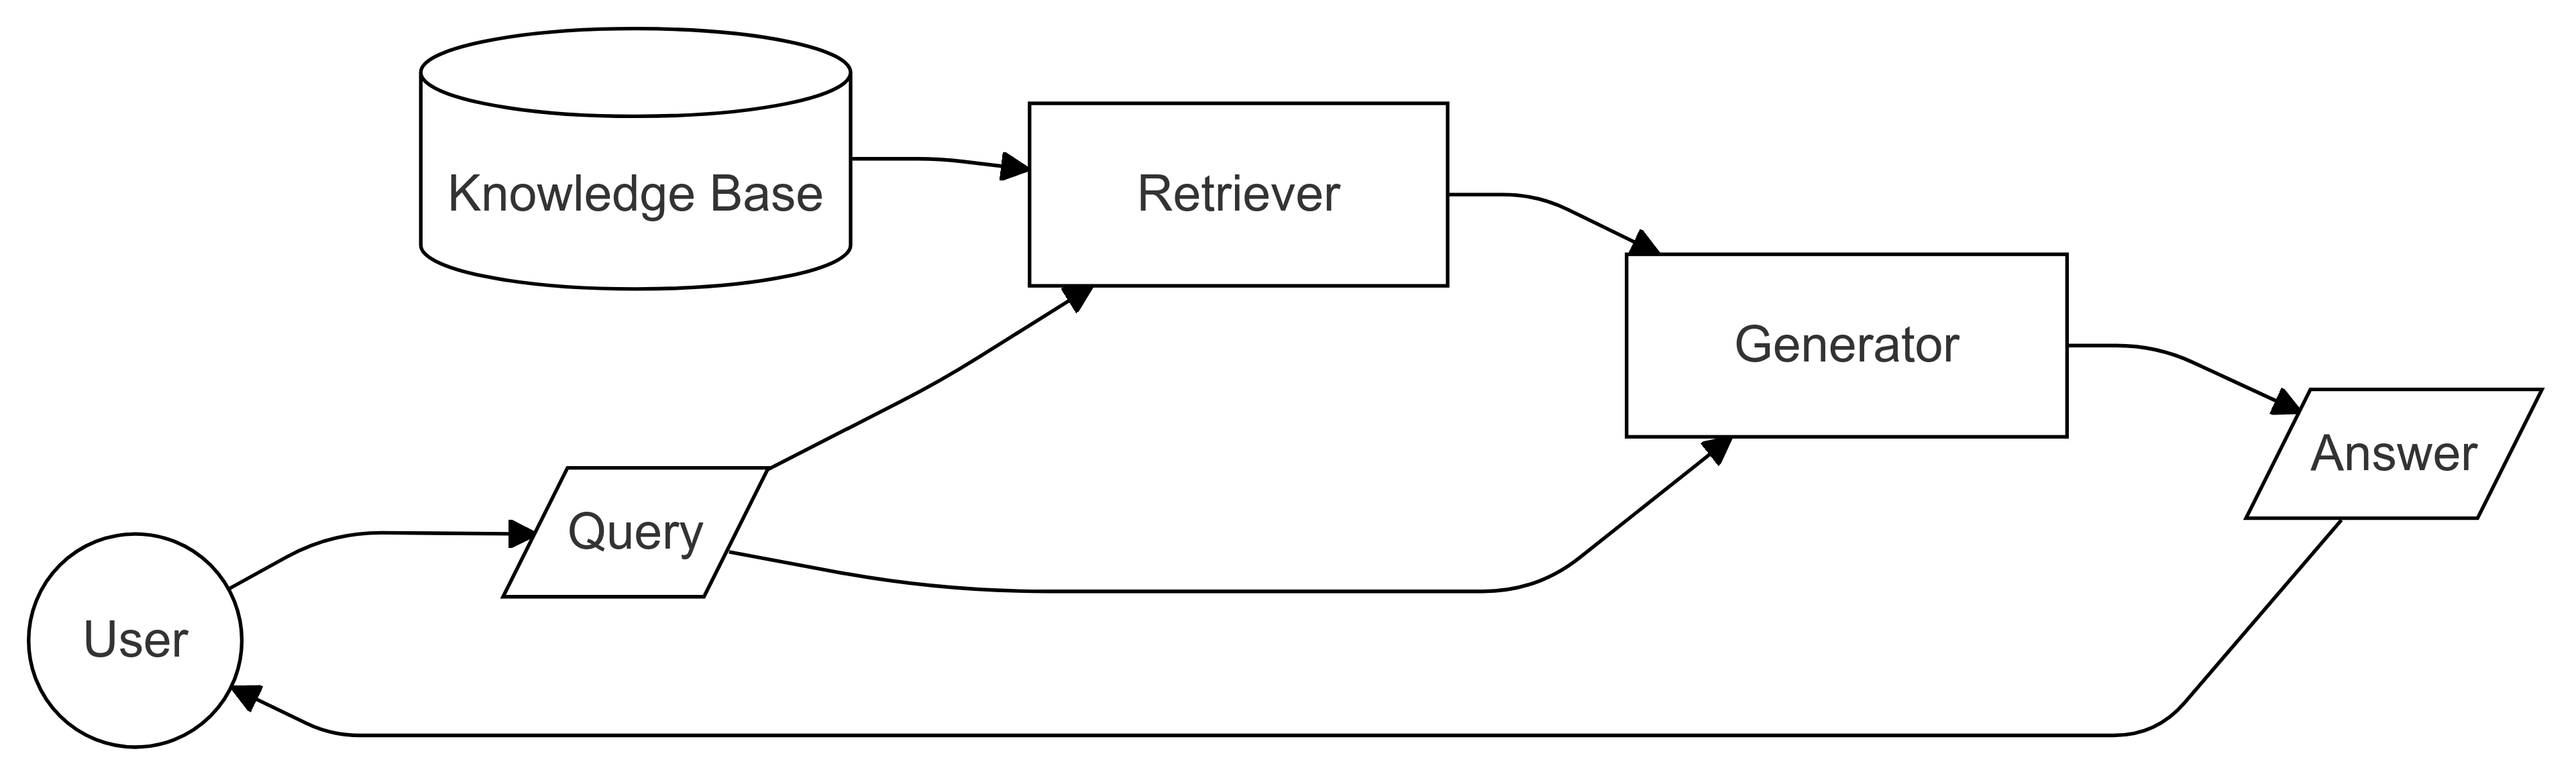
\includegraphics[width=0.8\textwidth]{figuras/rag-flow.png}
  \caption{Flujo de información en un sistema RAG}
  \label{fig:rag-flow}
\end{figure}

El proceso de generación sigue tres pasos fundamentales:

\begin{enumerate}
  \item \textbf{Recuperación de documentos relevantes}: El sistema vectoriza la consulta del usuario y busca en la base de conocimiento utilizando índices semánticos para encontrar documentos relacionados.

  \item \textbf{Análisis y ranking de documentos}: Se evalúa la relevancia de los documentos recuperados considerando su similitud semántica con la consulta y la confiabilidad de las fuentes.

  \item \textbf{Generación de respuestas}: El \gls{llm} integra el conocimiento recuperado con el contexto de la consulta para producir una respuesta coherente y precisa.
\end{enumerate}

\subsection{Aplicaciones y Ventajas de RAG en Educación}

Los sistemas \gls{rag} ofrecen beneficios significativos para aplicaciones educativas, especialmente en la enseñanza de idiomas. Las ventajas principales incluyen:

\begin{itemize}
  \item \textbf{Precisión y Confiabilidad:} Mayor precisión en la información proporcionada al combinar conocimiento estructurado con la flexibilidad de los \gls{llm}, reduciendo \gls{hallucinations} y respuestas incorrectas al anclar la generación en fuentes confiables.

  \item \textbf{Trazabilidad y Verificabilidad:} Capacidad de citar fuentes y materiales relevantes, proporcionando referencias verificables para el contenido educativo.

  \item \textbf{Adaptabilidad y Actualización:} estos sistemas ofrecen adaptabilidad a diferentes dominios mediante la actualización de la base de conocimiento. Esto permite una actualización dinámica del contenido sin necesidad de reentrenar el modelo completo. Además, facilita la personalización del contenido educativo mediante la selección específica de fuentes relevantes para cada estudiante.
\end{itemize}

\section{Aprendizaje por Refuerzo}

El Aprendizaje por Refuerzo (\gls{rl}) es una rama de la \gls{ia} que se enfoca en desarrollar agentes inteligentes capaces de aprender a través de la interacción con un entorno. Esta sección explora los fundamentos teóricos del \gls{rl} y su aplicación en el aprendizaje de idiomas.

\subsection{Fundamentos Teóricos del RL}

El Aprendizaje por Refuerzo proporciona un marco matemático ideal para la personalización del aprendizaje de idiomas. Basado en \gls{mdp}, permite modelar el proceso de aprendizaje como una serie de decisiones secuenciales, donde el sistema debe seleccionar las actividades y contenidos más apropiados según el nivel y progreso del estudiante \cite{williams2017educational}.

En nuestro contexto, el estado representa el perfil actual del estudiante, incluyendo su dominio del idioma en diferentes áreas (comprensión, producción, vocabulario, gramática), mientras que las acciones corresponden a las diferentes intervenciones pedagógicas disponibles.

\subsection{Proximal Policy Optimization (PPO)}

PPO \cite{schulman2017proximal} es un algoritmo de \gls{rl} que destaca por su estabilidad y eficiencia en el aprendizaje de políticas. En nuestro sistema de aprendizaje de idiomas, PPO se utiliza para optimizar la selección de actividades y la adaptación del contenido.


\subsubsection{Formulación Matemática}
El objetivo de PPO es maximizar la siguiente función objetivo:

\begin{equation}
  L^{CLIP}(\theta) = \hat{\mathbb{E}}_t[\min(r_t(\theta)\hat{A}_t, \text{clip}(r_t(\theta), 1-\epsilon, 1+\epsilon)\hat{A}_t)]
\end{equation}

Donde:

\begin{itemize}
  \item $r_t(\theta)$ es el ratio de probabilidades entre la política nueva y antigua
  \item $\hat{A}_t$ es la estimación de la ventaja
  \item $\epsilon$ es el parámetro de clipping (típicamente 0.2)
\end{itemize}

\begin{algorithm}[H]
  \label{alg2}
  \SetAlgoLined
  \medskip
  \begin{enumerate}
    \item Inicializar los parámetros de la política $\theta$ y el valor función $\phi$
    \item Para cada iteración:
          \begin{enumerate}
            \item Recopilar conjunto de trayectorias $\mathcal{D}_k = \{\tau_i\}$ ejecutando la política $\pi_\theta$ en el entorno
            \item Calcular ventajas estimadas $\hat{A}_t$ usando función de valor actual $V_\phi$
            \item Para cada época de optimización:
                  \begin{enumerate}
                    \item Calcular ratio de probabilidad $r_t(\theta) = \frac{\pi_\theta(a_t|s_t)}{\pi_{\theta_{old}}(a_t|s_t)}$
                    \item Calcular pérdida recortada:
                          $$L^{CLIP}(\theta) = \hat{\mathbb{E}}_t[\min(r_t(\theta)\hat{A}_t, \text{clip}(r_t(\theta), 1-\epsilon, 1+\epsilon)\hat{A}_t)]$$
                    \item Actualizar $\theta$ minimizando $-L^{CLIP}(\theta)$ usando descenso de gradiente
                    \item Actualizar función de valor $\phi$ minimizando error cuadrático medio
                  \end{enumerate}
            \item Actualizar $\theta_{old} \leftarrow \theta$
          \end{enumerate}
    \item Devolver la política optimizada $\pi_\theta$
  \end{enumerate}
  \caption{Algoritmo \textit{Proximal Policy Optimization} (PPO)}
\end{algorithm}

\subsubsection{Aplicación en el Sistema}

En nuestro contexto educativo:

\begin{itemize}
  \item \textbf{Estado ($\mathcal{S}$):} Representa el perfil actual del estudiante.
        \begin{equation}\label{eq:state}
          \mathcal{S} = \{\text{vocabulario\_nivel} = \text{B1}, \text{gramática\_nivel} = \text{A2}, \text{pronunciación\_nivel} = \text{B2}\}
        \end{equation}

  \item \textbf{Acciones ($\mathcal{A}$):} Selección de actividades y sus parámetros.
        \begin{equation}\label{eq:actions}
          \mathcal{A} = \{\text{ejercicio\_gramática\_A2}, \text{práctica\_vocabulario\_B1}, \text{diálogo\_pronunciación\_B2}\}
        \end{equation}

  \item \textbf{Recompensa ($\mathcal{R}$):} Evalúa el éxito de cada acción. Por ejemplo, si después de un ejercicio de gramática el estudiante mejora su precisión del 60\% al 80\%, $\mathcal{R} = +20$

  \item \textbf{Política ($\pi$):} Determina qué acción tomar en cada estado. Por ejemplo, si el estudiante muestra consistentemente errores en gramática, $\pi$ seleccionará más ejercicios gramaticales
\end{itemize}

\subsubsection{Sistema de Recompensas}

La \gls{reward-function} se diseña específicamente para el aprendizaje de idiomas, evaluando el desempeño y proporcionando retroalimentación a través de múltiples dimensiones:

\begin{itemize}
  \item \textbf{Recompensas inmediatas:} Incluyen la precisión en las respuestas y ejercicios, mejora en la pronunciación y fluidez, uso correcto de estructuras gramaticales, y la adquisición y retención de vocabulario.

  \item \textbf{Recompensas a largo plazo:} Consideran el progreso sostenido en múltiples dimensiones lingüísticas, la mejora en la competencia comunicativa general, y la retención y aplicación de conocimientos previos.

  \item \textbf{Ajustes dinámicos:} Comprenden la calibración automática de pesos de recompensa, adaptación a diferentes estilos y velocidades de aprendizaje, y el balanceo entre diferentes competencias lingüísticas.
\end{itemize}

\subsection{Evaluación de Políticas de Aprendizaje}

La evaluación de la \gls{policy} en sistemas de aprendizaje de idiomas requiere un enfoque multidimensional que considere tanto aspectos cuantitativos como cualitativos. \cite{williams2017educational} propone un marco de evaluación que examina:

\begin{itemize}
  \item \textbf{Progreso en competencias lingüísticas específicas:} Incluye la mejora en precisión gramatical y uso de estructuras, expansión del vocabulario activo y pasivo, desarrollo de fluidez y pronunciación, y avance en comprensión auditiva y lectora.

  \item \textbf{Efectividad de la personalización:} Abarca la adaptación a estilos individuales de aprendizaje, respuesta a patrones de error específicos, ajuste dinámico del nivel de dificultad y personalización de contenido temático.

  \item \textbf{Eficiencia en el tiempo de aprendizaje:} Considera la tasa de adquisición de nuevos conceptos, reducción en tiempo de dominio de habilidades, optimización de intervalos de repaso y minimización de redundancia en ejercicios.

  \item \textbf{Engagement y retención del estudiante:} Evalúa los niveles de participación activa, tasas de completación de actividades, persistencia en el programa de aprendizaje y satisfacción reportada por el estudiante.
\end{itemize}

La evaluación se realiza mediante métricas cuantitativas específicas:

\begin{equation}
  \text{Efectividad} = \frac{\text{Objetivos Alcanzados}}{\text{Tiempo Invertido}} \times \text{Factor de Dificultad}
\end{equation}

\begin{equation}
  \text{Índice de Personalización} = \frac{\sum_{i=1}^{n} \text{Adaptaciones Exitosas}_i}{n} \times \text{Tasa de Progreso}
\end{equation}

Estas métricas se complementan con análisis cualitativo continuo y retroalimentación directa de los estudiantes para asegurar una evaluación holística de la \gls{policy}.


\section{Tecnologías de Procesamiento de Voz}

El procesamiento de voz en sistemas de aprendizaje de idiomas involucra dos procesos fundamentales: el reconocimiento automático del habla (\gls{stt}) y la síntesis de voz (\gls{tts}). Estos procesos representan transformaciones complementarias entre el dominio acústico y el lingüístico.

\subsection{Reconocimiento Automático del Habla (STT)}

El proceso de STT transforma señales acústicas en texto, involucrando múltiples etapas de procesamiento y análisis. Este proceso se fundamenta en principios de procesamiento de señales y modelos probabilísticos del lenguaje \cite{graves2013speech}.

\subsubsection{Procesamiento de la Señal Acústica}

\begin{itemize}
  \item \textbf{Preprocesamiento Acústico:} La señal de audio cruda se somete a técnicas de reducción de ruido, normalización de amplitud y segmentación en tramas. Este proceso mejora la calidad de la señal y la prepara para el análisis posterior.

  \item \textbf{Extracción de Características:} Se extraen representaciones espectrales como coeficientes \gls{mfcc}, que capturan las características acústicas relevantes para el reconocimiento del habla.

  \item \textbf{Normalización de Características:} Las características extraídas se normalizan para reducir variaciones no lingüísticas como diferencias en el volumen o el canal de grabación.
\end{itemize}

\subsubsection{Proceso de Reconocimiento}

\begin{itemize}
  \item \textbf{Modelado Acústico:} Se analiza la relación entre las características acústicas y las unidades fonéticas del habla, considerando variaciones en pronunciación y contexto fonético.

  \item \textbf{Modelado del Lenguaje:} Se incorpora conocimiento sobre la estructura del lenguaje, incluyendo probabilidades de secuencias de palabras y restricciones gramaticales.

  \item \textbf{Decodificación:} Se combina la información acústica y lingüística para determinar la secuencia más probable de palabras, utilizando algoritmos de búsqueda como \gls{viterbi} o \gls{beam-search}.
\end{itemize}

\subsection{Síntesis de Voz (TTS)}

La síntesis de voz realiza la transformación inversa, convirtiendo texto en señales de habla mediante un proceso que combina análisis lingüístico y generación de señales acústicas \cite{taylor2009text}.


\subsubsection{Procesamiento Lingüístico}

\begin{itemize}
  \item \textbf{Análisis de Texto:} Se procesa el texto de entrada para identificar su estructura lingüística, incluyendo tokenización, normalización y análisis sintáctico.

  \item \textbf{Conversión Grafema-Fonema:} Se transforma el texto escrito en su representación fonética, considerando reglas de pronunciación y excepciones específicas del idioma.

  \item \textbf{Análisis Prosódico:} Se determinan patrones de entonación, duración y énfasis basados en la estructura sintáctica y semántica del texto.
\end{itemize}

\subsubsection{Generación de Voz}

\begin{itemize}
  \item \textbf{Modelado Prosódico:} Se generan patrones detallados de pitch, duración y energía para cada fonema, considerando el contexto lingüístico y emocional.

  \item \textbf{Generación de Características Acústicas:} Se producen representaciones espectrales intermedias que codifican las propiedades acústicas deseadas del habla.

  \item \textbf{Síntesis de Forma de Onda:} Se genera la señal de audio final mediante técnicas de síntesis que pueden ser concatenativas, paramétricas o basadas en modelos neuronales.
\end{itemize}

\subsection{Integración en Sistemas de Aprendizaje}

La combinación de STT y TTS en sistemas educativos permite crear ciclos completos de interacción oral:

\begin{itemize}
  \item \textbf{Ciclo de Retroalimentación:} El sistema puede generar ejemplos de pronunciación (TTS), analizar la producción del estudiante (STT) y proporcionar retroalimentación específica.

  \item \textbf{Análisis de Precisión:} La comparación entre la transcripción del habla del estudiante y el texto objetivo permite evaluar la precisión de pronunciación y fluidez.

  \item \textbf{Adaptación Dinámica:} Los resultados del análisis permiten ajustar parámetros como velocidad del habla, complejidad del contenido y umbral de aceptación de pronunciación.
\end{itemize}

La integración de estas tecnologías en sistemas de aprendizaje de idiomas permite una interacción más natural y efectiva, facilitando la práctica oral y la mejora de la competencia comunicativa de los estudiantes.



\chapter{Material}
\label{material}

Este capítulo detalla los recursos tecnológicos, infraestructura y herramientas utilizadas en el desarrollo del sistema de aprendizaje de idiomas. Se describe la arquitectura general, los componentes hardware y software, así como las bibliotecas y frameworks empleados.

\section{Infraestructura y Recursos Computacionales}

El sistema se implementa localmente utilizando una estación de trabajo de alto rendimiento, aprovechando las capacidades de aceleración por hardware para el procesamiento de modelos de lenguaje y voz.

\subsection{Recursos Hardware}

\begin{itemize}
	\item \textbf{GPU}: NVIDIA GeForce RTX 4070 con las siguientes características:
	      \begin{itemize}
		      \item 12GB de memoria VRAM GDDR6X
		      \item Soporte para CUDA y Tensor Cores
		      \item Capacidades de aceleración para \gls{ml} y \gls{ia}
	      \end{itemize}

	\item \textbf{Memoria Principal}:
	      \begin{itemize}
		      \item 32GB de RAM DDR4
		      \item Optimizada para cargas de trabajo intensivas en memoria
	      \end{itemize}

	\item \textbf{Almacenamiento}:
	      \begin{itemize}
		      \item 1TB SSD NVMe
		      \item Alto rendimiento en lectura/escritura
		      \item Almacenamiento de modelos y datos
	      \end{itemize}
\end{itemize}


\section{Componentes del Sistema}

El sistema se ha diseñado siguiendo una arquitectura modular y escalable que integra tecnologías de vanguardia en \gls{ia} y procesamiento de lenguaje natural. La arquitectura se divide en dos componentes principales: frontend y backend, comunicados a través de una \gls{api-rest}.

\subsection{Backend}

\begin{itemize}
	\item \textbf{LangChain}: Una herramienta poderosa para:
	      \begin{itemize}
		      \item Integrar modelos de lenguaje de gran escala (\gls{llm}) en el sistema
		      \item Gestionar y optimizar prompts para mejorar la interacción con los modelos de lenguaje
		      \item Procesar y analizar texto de manera eficiente utilizando técnicas avanzadas de procesamiento de lenguaje natural
		      \item Posibilita tener acceso a /gls{rag} para mejorar la precisión y relevancia de las respuestas generadas
	      \end{itemize}

	\item \textbf{FastAPI}: Un framework robusto para la creación de servicios de backend y la exposición de APIs, permitiendo una comunicación eficiente con el frontend:
	      \begin{itemize}
		      \item APIs REST de alto rendimiento y baja latencia
		      \item Generación automática de documentación interactiva mediante OpenAPI
		      \item Validación automática de datos y serialización eficiente
	      \end{itemize}
\end{itemize}

\subsubsection{Procesamiento de Voz}
\begin{itemize}
	\item \textbf{Faster-Whisper} (\cite{peng2024owsmv31betterfaster}): Motor de reconocimiento de voz que proporciona:
	      \begin{itemize}
		      \item Transcripción de audio a texto de alta precisión
		      \item Soporte multilingüe robusto
		      \item Optimización para CPU y GPU
	      \end{itemize}

	\item \textbf{Kokoro-TTS} (\cite{hexgrad_2025}): Sistema de síntesis de voz que ofrece:
	      \begin{itemize}
		      \item Generación de voz natural y expresiva
		      \item Múltiples voces y estilos
		      \item Alta eficiencia en el procesamiento
	      \end{itemize}
\end{itemize}

\subsubsection{Modelos de Lenguaje de Gran Escala (\gls{llm})}

\begin{itemize}
	\item \textbf{Phi-4 de Microsoft} (\cite{abdin2024phi4technicalreport}): Modelo avanzado de 14 mil millones de parámetros que impulsa las capacidades conversacionales del sistema:
		  \begin{itemize}
			  \item \textbf{Arquitectura y Entrenamiento}: Construido sobre una combinación estratégica de conjuntos de datos sintéticos, contenido web filtrado de dominio público, y recursos académicos especializados.
			  \item \textbf{Capacidad de Contexto}: 16,000 tokens, permitiendo mantener conversaciones extensas y retener información contextual relevante para el aprendizaje de idiomas.
			  \item \textbf{Ventajas para el Sistema}:
					\begin{itemize}
						\item Operación eficiente en entornos con restricciones computacionales.
						\item Baja latencia en interacciones conversacionales, crucial para la fluidez en el aprendizaje de idiomas.
						\item Capacidades avanzadas de razonamiento para análisis lingüísticos y correcciones gramaticales precisas.
						\item Generación de respuestas contextualmente apropiadas en múltiples idiomas.
					\end{itemize}
			  \item \textbf{Implementación en el Sistema}: El modelo se utiliza para:
					\begin{itemize}
						\item Generar diálogos educativos adaptados al nivel \gls{cefr} del estudiante.
						\item Analizar errores gramaticales y proporcionar retroalimentación pedagógica.
						\item Simular conversaciones auténticas en escenarios prácticos.
						\item Adaptar dinámicamente el contenido a las necesidades específicas del usuario.
					\end{itemize}
		  \end{itemize}

	\item \textbf{Nomic Embed} \cite{nussbaum2024nomic}: Modelo de embeddings de texto de alto rendimiento:
		\begin{itemize}
			\item \textbf{Características Principales}:
				\begin{itemize}
				  \item Ventana de contexto extendida de 8192 tokens
				  \item Modelo de código abierto bajo licencia Apache-2
				  \item Entrenamiento transparente con datos y código disponibles
				  \item Superior a OpenAI Ada-002 en benchmarks de contexto corto y largo
				\end{itemize}
			\item \textbf{Aplicación en el Sistema}:
				\begin{itemize}
				  \item Generación de embeddings para búsqueda semántica
				  \item Soporte a funcionalidades de RAG
				  \item Representación vectorial de conceptos lingüísticos
				  \item Análisis contextual de textos educativos
				\end{itemize}
		\end{itemize}
\end{itemize}

\section{Bases de Datos}

\begin{itemize}
	\item \textbf{Base de Datos SQL}: Almacenamiento de:
		  \begin{itemize}
			  \item Perfiles de usuarios: Información personal y preferencias de los usuarios.
			  \item Progreso de aprendizaje: Registro detallado del avance y desempeño de los usuarios en las actividades de aprendizaje.
			  \item Métricas de rendimiento: Datos estadísticos sobre el uso del sistema y la efectividad de las actividades de aprendizaje.
		  \end{itemize}

	\item \textbf{ChromaDB}: Base de datos vectorial para:
		  \begin{itemize}
			  \item Almacenamiento de embeddings: Representaciones vectoriales de datos textuales y de voz para facilitar la búsqueda y análisis.
			  \item Búsqueda semántica: Capacidad de realizar consultas basadas en el significado y contexto de los datos, en lugar de palabras clave exactas.
		      \item Recuperación de contexto: Extracción de información relevante y contextual para mejorar la interacción y respuestas del sistema.
	      \end{itemize}

	\item \textbf{Redis}: Sistema de caché en memoria para:
	      \begin{itemize}
		      \item Gestión de sesiones de usuario
		      \item Caché de respuestas frecuentes
		      \item Almacenamiento temporal de estados
	      \end{itemize}
\end{itemize}

\subsection{Frontend}

\begin{itemize}
	\item \textbf{Next.js}: Framework de React que ofrece:
	      \begin{itemize}
		      \item Renderizado híbrido (SSR y CSR): Permite la generación de contenido tanto en el servidor como en el cliente, mejorando el rendimiento y la experiencia del usuario.
		      \item Optimización automática de recursos: Gestión eficiente de imágenes, scripts y estilos para mejorar la velocidad de carga.
		      \item Soporte para API Routes: Facilita la creación de endpoints API directamente en la aplicación Next.js.
	      \end{itemize}


	\item \textbf{NextAuth.js}: Sistema de autenticación que proporciona:
	      \begin{itemize}
		      \item Múltiples proveedores de autenticación (OAuth, credenciales)
		      \item Gestión de sesiones segura
		      \item Integración con middleware de Next.js
	      \end{itemize}


	\item \textbf{Next-i18next}: Sistema de internacionalización que ofrece:
	      \begin{itemize}
		      \item Soporte para múltiples idiomas
		      \item Detección automática del idioma del navegador
		      \item Traducciones en el servidor y cliente
	      \end{itemize}
\end{itemize}

\section{Recursos Lingüísticos}

\subsection{Modelos de Voz}
\begin{itemize}
	\item \textbf{Síntesis de Voz (\gls{tts})}:
	      \begin{itemize}
		      \item Generación de voz natural y fluida mediante Kokoro-TTS
		      \item Soporte para 8 idiomas principales:
		            \begin{itemize}
			            \item Inglés (en)
			            \item Español (es)
			            \item Francés (fr)
			            \item Hindi (hi)
			            \item Italiano (it)
			            \item Portugués (pt)
			            \item Japonés (ja)
			            \item Chino (zh)
		            \end{itemize}
		      \item Personalización de voces y estilos de habla
		      \item Optimización para diferentes contextos conversacionales
	      \end{itemize}

	\item \textbf{Reconocimiento de Voz (\gls{stt})}:
	      \begin{itemize}
		      \item Transcripción precisa mediante Faster-Whisper
		      \item Soporte extendido para 20 idiomas:
		            \begin{itemize}
			            \item Lenguas germánicas: Inglés, Alemán, Holandés, Danés, Sueco
			            \item Lenguas románicas: Español, Francés, Italiano, Portugués, Rumano
			            \item Lenguas eslavas: Checo, Polaco, Ruso, Ucraniano
			            \item Lenguas asiáticas: Hindi, Japonés, Coreano, Chino
			            \item Otras lenguas: Árabe, Turco
		            \end{itemize}
		      \item Procesamiento optimizado para CPU y GPU
		      \item Alta precisión en diversos acentos y dialectos
	      \end{itemize}
\end{itemize}


\subsection{Recursos Educativos}
\begin{itemize}
	\item \textbf{Material Didáctico CEFR}:
	      \begin{itemize}
		      \item Contenidos alineados con niveles A1 a C2 del Marco Común Europeo
		      \item Progresión gradual y estructurada del aprendizaje
		      \item Generación sintética de frases adaptadas al nivel \gls{cefr}:
		            \begin{itemize}
			            \item Vocabulario controlado por nivel
			            \item Estructuras gramaticales graduadas
			            \item Complejidad léxica adaptativa
		            \end{itemize}
	      \end{itemize}

	\item \textbf{Escenarios de Práctica}:
	      \begin{itemize}
		      \item Situaciones comunes predefinidas para role-play:
		            \begin{itemize}
			            \item Encuentros sociales básicos
			            \item Transacciones comerciales
			            \item Situaciones profesionales
			            \item Contextos académicos
			            \item Emergencias y asistencia
		            \end{itemize}
		      \item Ejercicios interactivos graduados:
		            \begin{itemize}
			            \item Comprensión lectora y auditiva
			            \item Producción oral y escrita
			            \item Retroalimentación personalizada en tiempo real
		            \end{itemize}
		      \item Práctica contextualizada:
		            \begin{itemize}
			            \item Escenarios de la vida real
			            \item Diálogos situacionales
			            \item Simulaciones de conversaciones auténticas
		            \end{itemize}
	      \end{itemize}
\end{itemize}

\chapter{Métodos}
\label{metodos}

Este capítulo describe la metodología empleada en el desarrollo del sistema de aprendizaje de idiomas, incluyendo la arquitectura del sistema, la implementación de los componentes, los algoritmos desarrollados y la metodología de evaluación.

\section{Arquitectura del Sistema}
\label{arquitectura-sistema}

El sistema se ha diseñado siguiendo una arquitectura modular y escalable que integra tecnologías de vanguardia en \gls{ia} y procesamiento de lenguaje natural. La arquitectura se divide en dos componentes principales: frontend y backend, comunicados a través de una API REST.

\begin{figure}[H]
	\centering
	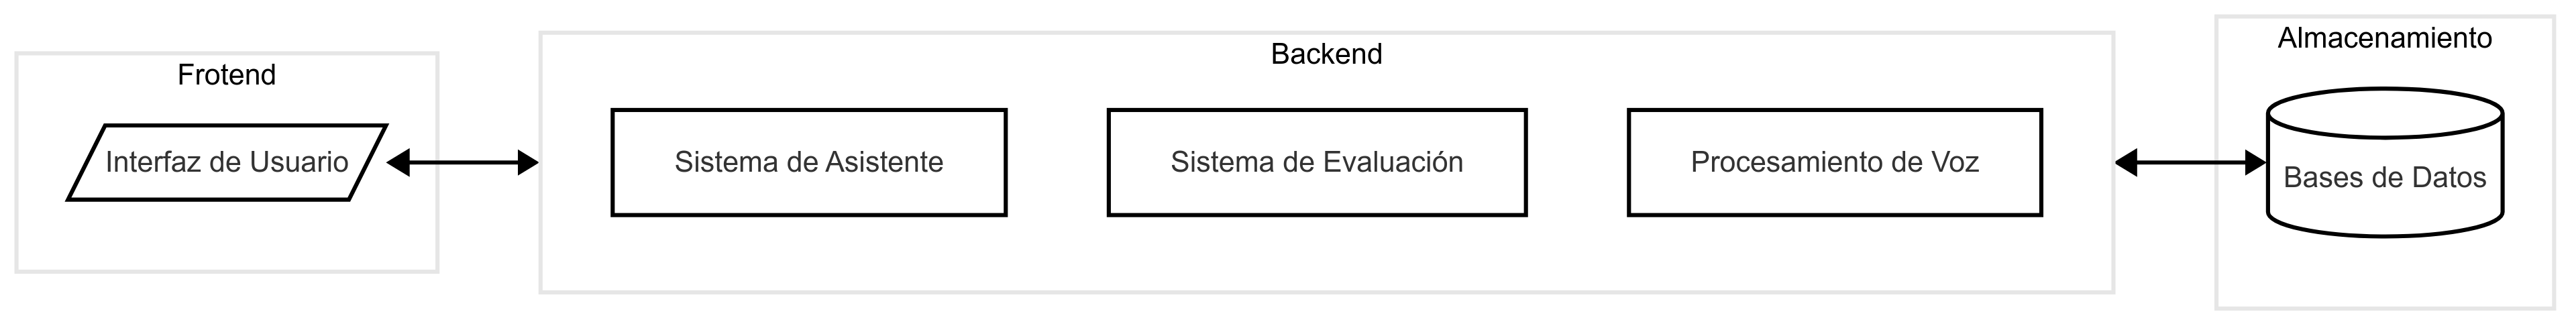
\includegraphics[width=0.8\textwidth]{figuras/system-overview.png}
	\caption{Arquitectura Simplificada del Sistema}
	\label{fig:arquitectura-sistema}
\end{figure}


\subsection{Frontend}
\label{frontend}

El frontend del sistema se implementa utilizando Next.js y está basado en el framework \gls{assistant-ui}, un proyecto \gls{open-source} que facilita la integración de interfaces de chat con LangGraph. Esta decisión arquitectónica permite una rápida implementación de funcionalidades de chat mientras mantiene la flexibilidad para personalizaciones específicas del dominio.

\begin{figure}[H]
	\centering
	\caption{Arquitectura del Frontend}
	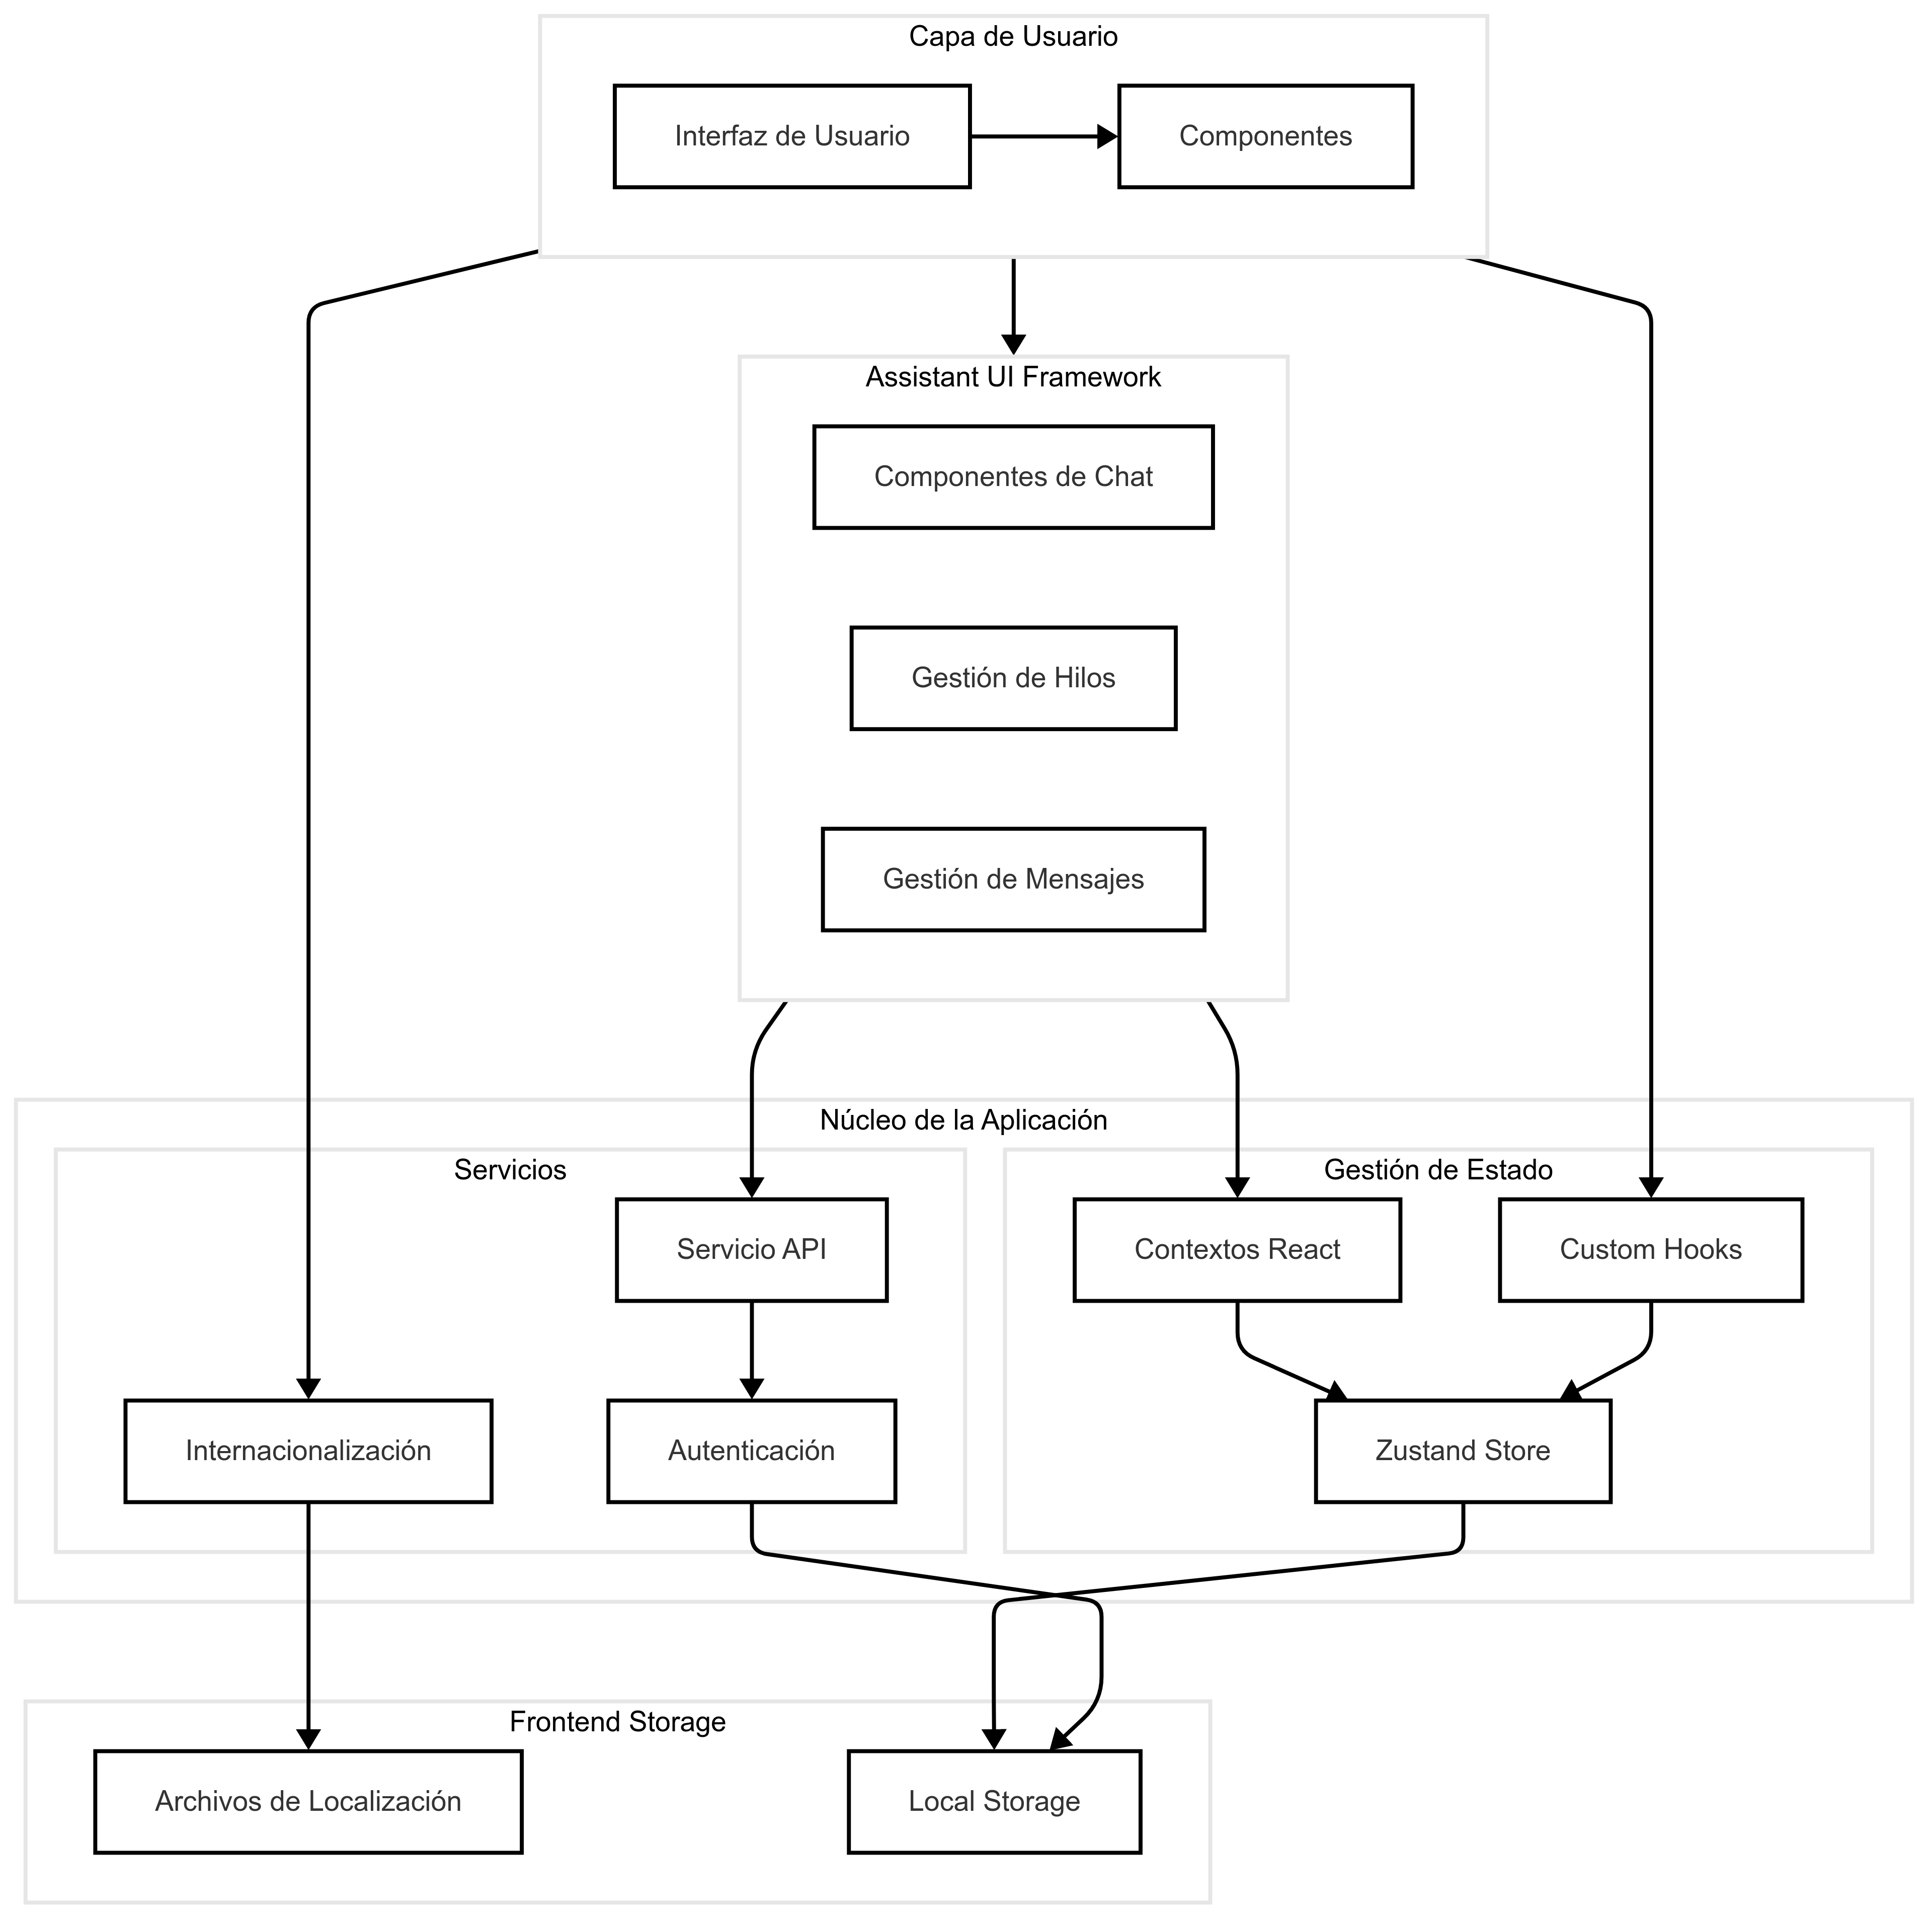
\includegraphics[width=0.8\textwidth]{figuras/frontend.png}
	\label{fig:arquitectura-frontend}
\end{figure}

\subsubsection{Assistant UI Framework}
\label{assistant-ui}

El sistema se construye sobre \gls{assistant-ui}, que proporciona:

\begin{itemize}
	\item \textbf{Componentes de Chat}:
	      \begin{itemize}
		      \item Interfaz de chat prediseñada y personalizable
		      \item Sistema de renderizado de mensajes
		      \item Gestión de entrada de usuario
	      \end{itemize}

	\item \textbf{Gestión de Hilos}:
	      \begin{itemize}
		      \item Sistema de hilos de conversación
		      \item Persistencia de contexto conversacional
		      \item Manejo de múltiples conversaciones
	      \end{itemize}

	\item \textbf{Gestión de Mensajes}:
	      \begin{itemize}
		      \item Sistema de cola de mensajes
		      \item Gestión de estados de mensajes
		      \item Manejo de respuestas asíncronas
	      \end{itemize}
\end{itemize}
\subsubsection{Arquitectura de Componentes}
La arquitectura del frontend se organiza en las siguientes capas:

\begin{itemize}
	\item \textbf{Capa de Usuario}:
	      \begin{itemize}
		      \item Implementación de páginas y rutas utilizando el sistema de enrutamiento de Next.js
		      \item Implementación de layouts y templates adaptables
		      \item Integración con el sistema de internacionalización
	      \end{itemize}

	\item \textbf{Núcleo de la Aplicación}:
	      \begin{itemize}
		      \item Gestión de estado utilizando Zustand para el manejo de datos de roleplay, progreso y reportes
		      \item Servicios para comunicación con el backend
		      \item Sistema de internacionalización con archivos de localización
	      \end{itemize}

	\item \textbf{Utilidades}:
	      \begin{itemize}
		      \item Funciones de validación y formateo
		      \item Manejadores de errores globales
		      \item Helpers para formateo y transformación de datos
		      \item Adaptadores para internacionalización
	      \end{itemize}
\end{itemize}

\subsubsection{Gestión de Estado}
\label{gestion-estado}

El sistema utiliza Zustand como solución de gestión de estado, proporcionando:

\begin{itemize}
	\item \textbf{Estado Global}:
	      \begin{itemize}
		      \item Gestión del estado del roleplay
		      \item Seguimiento del progreso del usuario
		      \item Almacenamiento de reportes de actividad
	      \end{itemize}

	\item \textbf{Persistencia}:
	      \begin{itemize}
		      \item Integración con localStorage para persistencia de datos
		      \item Sincronización de estado entre sesiones
		      \item Gestión de caché de datos
	      \end{itemize}
\end{itemize}

\subsubsection{Servicios de Comunicación}
\label{servicios-comunicacion}

La comunicación con el backend se gestiona a través de servicios especializados:

\begin{itemize}
	\item \textbf{API Service}:
	      \begin{itemize}
		      \item Implementación de cliente HTTP basado en Axios
		      \item Sistema de interceptores para manejo de errores
		      \item Caché de respuestas para optimización de rendimiento
	      \end{itemize}

	\item \textbf{Gestión de Autenticación}:
	      \begin{itemize}
		      \item Sistema de autenticación basado en tokens
		      \item Manejo de sesiones de usuario
		      \item Protección de rutas y recursos
	      \end{itemize}

	\item \textbf{Servicio de Internacionalización}:
	      \begin{itemize}
		      \item Gestión de traducciones y locales
		      \item Cambio dinámico de idioma
		      \item Formateo de fechas y números según la localización
	      \end{itemize}
\end{itemize}

\subsection{Backend}
\label{backend}

El backend del sistema se implementa utilizando FastAPI como framework principal, incorporando un sistema multi-agente basado en LangGraph para la gestión de la lógica de aprendizaje. La arquitectura se organiza en capas claramente definidas que gestionan diferentes aspectos del sistema.

\begin{figure}[H]
	\centering
	\caption{Arquitectura del Backend}
	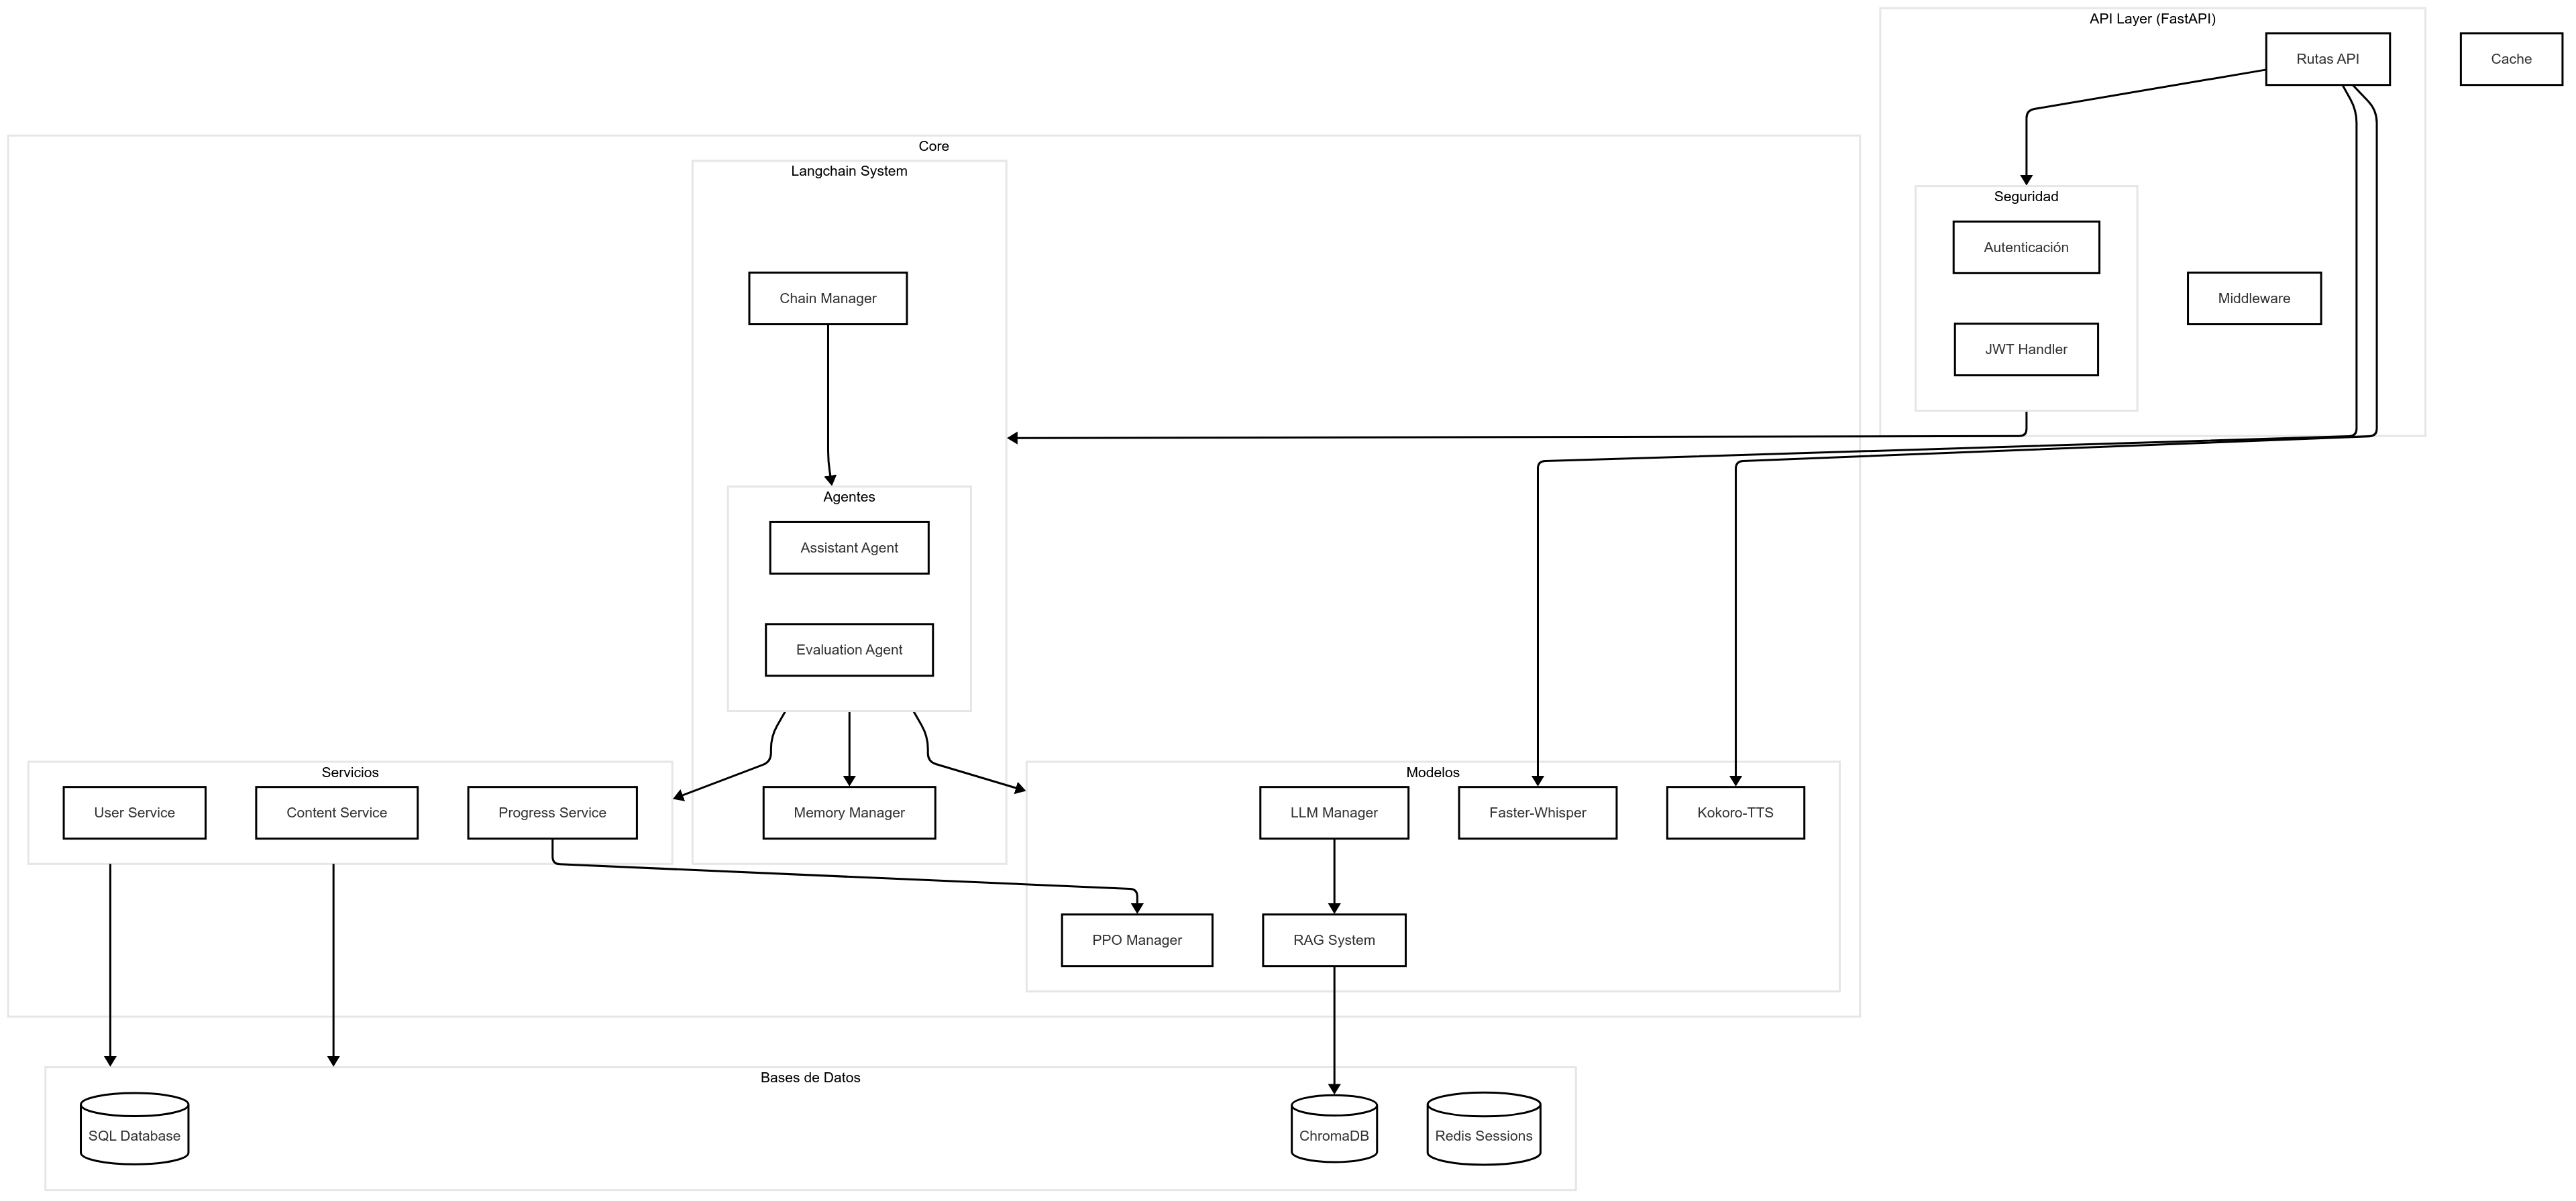
\includegraphics[width=0.8\textwidth]{figuras/backend.png}
	\label{fig:arquitectura-backend}
\end{figure}

\subsubsection{Capa de API}
\label{capa-api}

La capa de API, implementada con FastAPI, gestiona todas las interacciones con el cliente a través de endpoints RESTful. El sistema proporciona:

\begin{itemize}
    \item \textbf{Documentación y Validación}:
    \begin{itemize}
        \item Documentación automática mediante OpenAPI
        \item Validación de datos utilizando Pydantic
    \end{itemize}

    \item \textbf{Seguridad}:
    \begin{itemize}
        \item Autenticación mediante JWT
        \item Rate limiting para prevención de abusos
        \item Sistema de validación de permisos basado en roles
        \item Implementación de CORS para seguridad entre dominios
    \end{itemize}

    \item \textbf{Procesamiento de Voz}:
    \begin{itemize}
        \item Integración con Faster-Whisper para transcripción de voz
        \item Integración con Kokoro-TTS para síntesis de voz
    \end{itemize}
\end{itemize}
\subsubsection{Sistema Multi-Agente}
\label{sistema-multi-agente}

El sistema implementa dos agentes especializados utilizando Langchain:

\begin{itemize}
    \item \textbf{Assistant Agent}: Maneja las conversaciones con el usuario, integrándose con modelos \gls{llm} y utilizando un sistema de \gls{rag} para contextualización.
    
    \item \textbf{Evaluation Agent}: Realiza la evaluación continua del progreso, analiza patrones de error y ajusta los parámetros de aprendizaje utilizando el modelo \gls{ppo}.
\end{itemize}

\subsubsection{Gestión de Modelos}
\label{gestion-modelos}

La integración de modelos de \gls{ia} se realiza a través de gestores especializados:

\begin{itemize}
    \item \textbf{LLM Manager}: Coordina la integración con modelos de lenguaje, gestionando prompts y contextos.
    
    \item \textbf{PPO Manager}: Implementa el algoritmo \gls{ppo}, manejando estados y recompensas para la evaluación.
    
    \item \textbf{RAG System}: Gestiona la indexación de contenido educativo y realiza búsquedas semánticas mediante ChromaDB.
    
    \item \textbf{Modelos de Voz}: Implementa Faster-Whisper para STT y Kokoro-TTS para TTS.
\end{itemize}

\subsubsection{Servicios Core}
\label{servicios-core}

Los servicios principales del sistema incluyen:

\begin{itemize}
    \item \textbf{User Service}: Gestiona perfiles de usuario y preferencias.
    
    \item \textbf{Content Service}: Maneja la gestión y adaptación de recursos educativos.
    
    \item \textbf{Progress Service}: Realiza el seguimiento del avance y se integra con el modelo PPO para la evaluación.
\end{itemize}

\subsubsection{Capa de Datos}
\label{capa-datos}

La gestión de datos se implementa mediante tres sistemas de almacenamiento:

\begin{itemize}
    \item \textbf{SQL Database}: Almacena datos estructurados y relaciones entre entidades.
    
    \item \textbf{ChromaDB}: Base de datos vectorial para embeddings y búsquedas semánticas.
    
    \item \textbf{Redis}: Gestión de sesiones y caché para optimizar el acceso a datos frecuentes.
\end{itemize}

\subsubsection{Optimización y Monitoreo}
\label{optimizacion-monitoreo}

El sistema implementa:

\begin{itemize}
    \item \textbf{Monitoreo}:
    \begin{itemize}
        \item Logging estructurado de eventos
        \item Métricas de rendimiento
        \item Sistema de alertas automáticas
    \end{itemize}

    \item \textbf{Optimización}:
    \begin{itemize}
        \item Caché en múltiples niveles
        \item Pooling de conexiones
        \item Arquitectura stateless
    \end{itemize}
\end{itemize}


\section{Implementación de los Componentes}
\label{implementacion-componentes}

Esta sección detalla la implementación técnica de los componentes principales del sistema: el sistema de agentes y el procesamiento de voz. Cada componente se ha desarrollado considerando los requisitos de rendimiento, escalabilidad y usabilidad del sistema.

\subsection{Sistema de Agentes}
\label{implementacion-agentes}

El sistema implementa dos agentes especializados utilizando Langchain como framework base. Cada agente está diseñado con responsabilidades específicas y utiliza el sistema de memoria de Langchain para mantener el contexto de las interacciones.

\subsubsection{Assistant Agent}

El Assistant Agent se construye sobre un modelo \gls{llm} con un sistema de \gls{rag} para contextualización. Sus principales componentes son:

\begin{itemize}
    \item \textbf{Gestión de Contexto}:
    \begin{itemize}
        \item Mantiene el estado del diálogo mediante el Memory Manager de Langchain
        \item Implementa un sistema de recuperación de contexto relevante
        \item Coordina la integración con el sistema RAG
    \end{itemize}

    \item \textbf{Generación de Respuestas}:
    \begin{itemize}
        \item Utiliza templates dinámicos adaptados al nivel del estudiante
        \item Implementa prompts específicos para diferentes tipos de interacciones
        \item Mantiene la coherencia pedagógica en las conversaciones
    \end{itemize}

    \item \textbf{Integración con Servicios}:
    \begin{itemize}
        \item Coordina con el Content Service para acceso a recursos educativos
        \item Interactúa con el User Service para personalización
        \item Registra interacciones para análisis posterior
    \end{itemize}
\end{itemize}

\subsubsection{Evaluation Agent}

El Evaluation Agent implementa un sistema de evaluación continua que utiliza el modelo \gls{ppo} para optimizar las evaluaciones. Sus componentes principales incluyen:

\begin{itemize}
    \item \textbf{Sistema de Evaluación}:
    \begin{itemize}
        \item Implementa métricas para diferentes aspectos del aprendizaje
        \item Utiliza \gls{ppo} para ajustar los parámetros de evaluación
        \item Mantiene un registro detallado del progreso del estudiante
    \end{itemize}

    \item \textbf{Análisis de Progreso}:
    \begin{itemize}
        \item Evalúa la precisión lingüística en las interacciones
        \item Determina niveles de competencia en diferentes habilidades
        \item Genera informes de progreso personalizados
    \end{itemize}

    \item \textbf{Integración con Servicios}:
    \begin{itemize}
        \item Coordina con el Progress Service para el seguimiento
        \item Alimenta el sistema PPO con datos de rendimiento
        \item Mantiene métricas de evaluación en la base de datos
    \end{itemize}
\end{itemize}

\subsubsection{Comunicación entre Agentes}

La comunicación y coordinación entre agentes se implementa mediante:

\begin{itemize}
    \item \textbf{Chain Manager}:
    \begin{itemize}
        \item Coordina el flujo de información entre agentes
        \item Gestiona la secuencia de operaciones
        \item Mantiene la consistencia del estado del sistema
    \end{itemize}

    \item \textbf{Memory Manager}:
    \begin{itemize}
        \item Gestiona el estado compartido entre agentes
        \item Implementa diferentes tipos de memoria según la necesidad
        \item Mantiene la persistencia del contexto conversacional
    \end{itemize}

    \item \textbf{Validación de Datos}:
    \begin{itemize}
        \item Utiliza Pydantic para validación de tipos
        \item Incluye metadatos como timestamps y tipos de interacción
        \item Facilita el debugging y monitoreo del sistema
    \end{itemize}
\end{itemize}

\subsection{Procesamiento de Voz}
\label{implementacion-voz}

El procesamiento de voz se implementa en el backend utilizando Faster-Whisper para el reconocimiento de voz y Kokoro-TTS para la síntesis de voz. El sistema se divide en dos pipelines principales: reconocimiento y síntesis de voz.

\subsubsection{Pipeline de Reconocimiento de Voz}

El sistema de reconocimiento de voz utiliza Faster-Whisper, una implementación optimizada del modelo Whisper de OpenAI. Sus características principales incluyen:

\begin{itemize}
    \item \textbf{Preprocesamiento de Audio}:
    \begin{itemize}
        \item Normalización de la señal de audio
        \item Detección automática de segmentos de voz
        \item Filtrado de ruido y mejora de la señal
    \end{itemize}

    \item \textbf{Optimizaciones de Rendimiento}:
    \begin{itemize}
        \item Implementación en CTranslate2 para mayor velocidad
        \item Procesamiento por lotes eficiente
        \item Cuantización del modelo para optimizar memoria
    \end{itemize}

    \item \textbf{Características Avanzadas}:
    \begin{itemize}
        \item Detección automática de idioma
        \item Timestamps para alineación de texto
        \item Soporte para transcripción en tiempo real
    \end{itemize}
\end{itemize}

\subsubsection{Pipeline de Síntesis de Voz}

La síntesis de voz se realiza mediante Kokoro-TTS, un sistema avanzado de text-to-speech. Sus componentes principales son:

\begin{itemize}
    \item \textbf{Procesamiento de Texto}:
    \begin{itemize}
        \item Análisis lingüístico del texto de entrada
        \item Normalización de texto y números
        \item Procesamiento de símbolos especiales y abreviaturas
    \end{itemize}

    \item \textbf{Generación de Voz}:
    \begin{itemize}
        \item Síntesis de voz de alta calidad
        \item Control de entonación y prosodia
        \item Ajuste de velocidad y tono
    \end{itemize}

    \item \textbf{Optimizaciones}:
    \begin{itemize}
        \item Sistema de caché para frases frecuentes
        \item Streaming de audio para respuesta rápida
        \item Gestión eficiente de recursos del servidor
    \end{itemize}
\end{itemize}

\section{Algoritmos Desarrollados}
\label{algoritmos-desarrollados}

Esta sección detalla los algoritmos principales desarrollados para la personalización del aprendizaje, incluyendo el sistema de \gls{rl} y el mecanismo de recompensas.

\begin{figure}[H]
	\caption{Flujo del Algoritmo de RL y Sistema de Recompensas}
	\label{fig:rl-flow}
	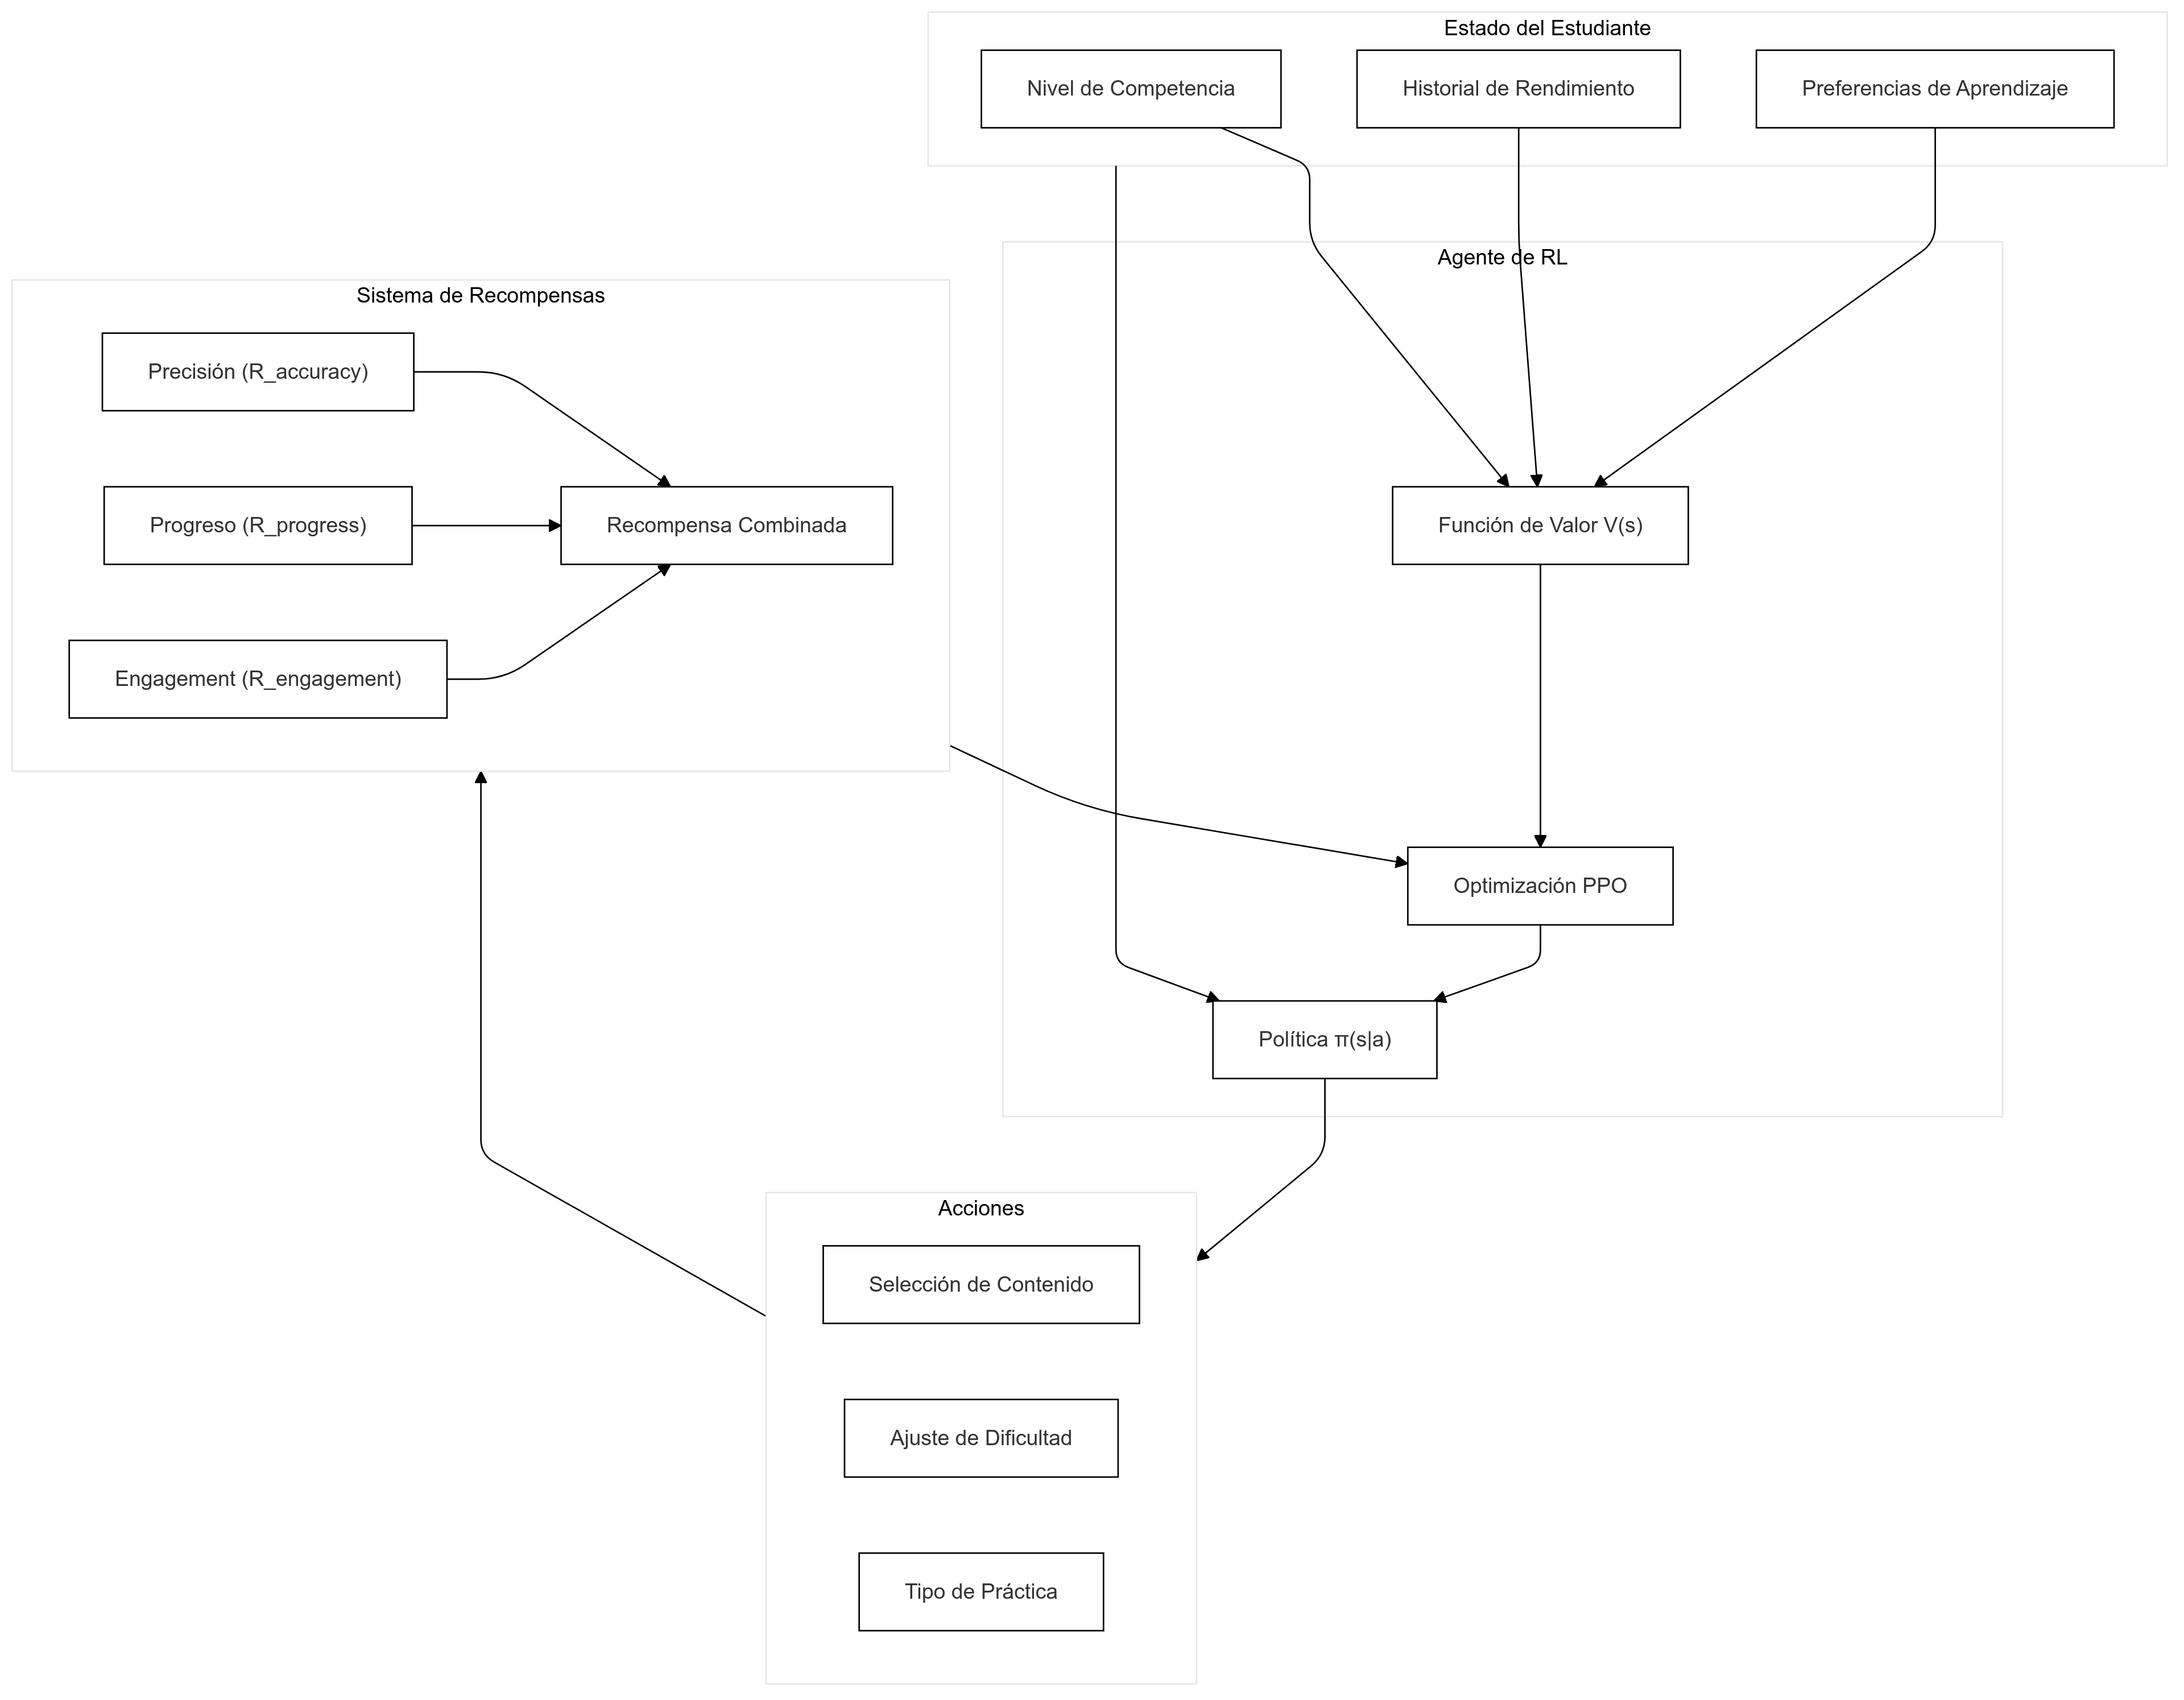
\includegraphics[width=0.8\textwidth]{figuras/rl-flow.png}
\end{figure}

\subsection{Algoritmo de Personalización}
\label{algoritmo-personalizacion}

El sistema implementa un algoritmo de \gls{rl} basado en \gls{ppo} \cite{schulman2017proximal} para optimizar las rutas de aprendizaje. El objetivo es maximizar el aprendizaje a largo plazo mientras se mantiene un nivel apropiado de desafío y engagement.

\subsubsection{Formulación del Problema}

El problema se formula como un \gls{mdp} donde:

\begin{itemize}
	\item \textbf{Estado ($s_t$):} Vector que representa el estado actual del estudiante:
	      \begin{equation}
		      s_t = [c_1, ..., c_n, h_1, ..., h_m, p_1, ..., p_k]
	      \end{equation}
	      donde $c_i$ son los niveles de competencia en diferentes habilidades, $h_i$ es el historial de rendimiento, y $p_i$ son las preferencias de aprendizaje.

	\item \textbf{Acciones ($a_t$):} Vector de decisiones pedagógicas:
	      \begin{equation}
		      a_t = [d, t, c]
	      \end{equation}
	      donde $d$ es el nivel de dificultad, $t$ es el tipo de ejercicio, y $c$ es el contenido específico.

	\item \textbf{Política ($\pi_\theta$):} La política que mapea estados a acciones:
	      \begin{equation}
		      \pi_\theta(a_t|s_t) = P(a_t|s_t; \theta)
	      \end{equation}
\end{itemize}

\subsubsection{Algoritmo PPO}

El algoritmo PPO optimiza la política mediante la siguiente función objetivo:

\begin{equation}
	\label{eq:ppo-objective}
	L^{CLIP}(\theta) = \mathbb{E}_t[\min(r_t(\theta)A_t, \text{clip}(r_t(\theta), 1-\epsilon, 1+\epsilon)A_t)]
\end{equation}

donde:
\begin{itemize}
	\item $r_t(\theta) = \frac{\pi_\theta(a_t|s_t)}{\pi_{\theta_{old}}(a_t|s_t)}$ es el ratio de probabilidades
	\item $A_t$ es la estimación de ventaja
	\item $\epsilon$ es el parámetro de recorte (típicamente 0.2)
\end{itemize}

La actualización de la política se realiza mediante descenso de gradiente:

\begin{equation}
	\theta_{new} = \theta + \alpha \nabla_\theta L^{CLIP}(\theta)
\end{equation}

\subsection{Sistema de Recompensas}
\label{sistema-recompensas}

Se implementa un sistema de recompensas multiobjetivo que considera tres componentes principales:

\begin{equation}
	\label{eq:reward}
	R = w_1R_{accuracy} + w_2R_{progress} + w_3R_{engagement}
\end{equation}

\subsubsection{Componentes de Recompensa}

\begin{itemize}
	\item \textbf{Precisión ($R_{accuracy}$):} Evalúa la corrección de las respuestas:
	      \begin{equation}
		      R_{accuracy} = \frac{\text{respuestas\_correctas}}{\text{total\_respuestas}} \cdot \gamma
	      \end{equation}
	      donde $\gamma$ es un factor de dificultad que aumenta la recompensa para ejercicios más desafiantes.

	\item \textbf{Progreso ($R_{progress}$):} Mide el avance en el dominio de habilidades:
	      \begin{equation}
		      R_{progress} = \sum_{i=1}^n \Delta c_i \cdot \beta_i
	      \end{equation}
	      donde $\Delta c_i$ es el cambio en el nivel de competencia de la habilidad $i$, y $\beta_i$ es su peso relativo.

	\item \textbf{Engagement ($R_{engagement}$):} Evalúa la participación activa:
	      \begin{equation}
		      R_{engagement} = \alpha_t t_{session} + \alpha_c c_{completion} + \alpha_i i_{interaction}
	      \end{equation}
	      donde $t_{session}$ es la duración de la sesión, $c_{completion}$ es la tasa de finalización, y $i_{interaction}$ es la frecuencia de interacción.
\end{itemize}

\subsubsection{Adaptación de Pesos}

Los pesos $w_i$ se ajustan dinámicamente según el perfil del estudiante mediante un algoritmo de adaptación:

\begin{equation}
	w_i^{new} = w_i + \eta(\bar{R}_i - R_{target}) + \lambda\Delta w_i
\end{equation}

donde:
\begin{itemize}
	\item $\eta$ es la tasa de adaptación
	\item $\bar{R}_i$ es la recompensa promedio reciente para el componente $i$
	\item $R_{target}$ es el valor objetivo
	\item $\lambda\Delta w_i$ es un término de momentum para estabilizar los cambios
\end{itemize}

\section{Metodología de Evaluación}
\label{metodologia-evaluacion}

La evaluación del sistema se realiza en dos dimensiones principales: rendimiento técnico y experiencia de usuario. Este enfoque permite valorar tanto la eficiencia técnica del sistema como su utilidad práctica para los usuarios.

\subsection{Evaluación de Rendimiento}
\label{evaluacion-rendimiento}

La evaluación técnica del sistema se centra en dos aspectos principales:

\subsubsection{Métricas del Sistema}

\begin{itemize}
	\item \textbf{Latencia de Respuesta:} Se mide el tiempo de respuesta del sistema en diferentes puntos:
	      \begin{itemize}
		      \item Tiempo de procesamiento de solicitudes API
		      \item Latencia en la generación de respuestas
		      \item Tiempo de renderizado en el cliente
	      \end{itemize}

	\item \textbf{Uso de Recursos:}
	      \begin{itemize}
		      \item Consumo de memoria en el cliente
		      \item Utilización de CPU/GPU
		      \item Eficiencia en el uso de WebGPU
	      \end{itemize}
\end{itemize}

\subsubsection{Rendimiento del Procesamiento de Voz}

\begin{itemize}
	\item \textbf{Precisión en Reconocimiento de Voz:}
	      \begin{itemize}
		      \item Tasa de error en la transcripción
		      \item Precisión en diferentes entornos acústicos
		      \item Tiempo de procesamiento
	      \end{itemize}

	\item \textbf{Calidad de Síntesis de Voz:}
	      \begin{itemize}
		      \item Naturalidad de la voz generada
		      \item Consistencia en la pronunciación
		      \item Velocidad de generación
	      \end{itemize}
\end{itemize}

\subsection{Evaluación de Usuario}
\label{evaluacion-usuario}

La evaluación de la experiencia de usuario se realiza mediante un proceso continuo que combina análisis cuantitativo y cualitativo.

\subsubsection{Recopilación de Retroalimentación}

\begin{itemize}
	\item \textbf{Encuestas de Usuario:}
	      \begin{itemize}
		      \item Evaluación de la facilidad de uso
		      \item Satisfacción con las funcionalidades
		      \item Percepción de la utilidad del sistema
	      \end{itemize}

	\item \textbf{Datos Cualitativos:}
	      \begin{itemize}
		      \item Comentarios y sugerencias de usuarios
		      \item Reportes de problemas
		      \item Sugerencias de mejora
	      \end{itemize}
\end{itemize}

\subsubsection{Análisis de Patrones de Uso}

\begin{itemize}
	\item \textbf{Métricas de Uso:}
	      \begin{itemize}
		      \item Duración promedio de las sesiones
		      \item Frecuencia de uso
		      \item Patrones de interacción
	      \end{itemize}

	\item \textbf{Análisis de Comportamiento:}
	      \begin{itemize}
		      \item Funcionalidades más utilizadas
		      \item Puntos de abandono
		      \item Patrones de navegación
	      \end{itemize}
\end{itemize}

\subsection{Análisis de Resultados}

Los resultados de estas evaluaciones se utilizarán para:

\begin{itemize}
	\item Identificar y corregir problemas técnicos
	\item Mejorar la experiencia de usuario
	\item Optimizar el rendimiento del sistema
	\item Guiar el desarrollo de futuras funcionalidades
\end{itemize}
\chapter{Resultados}
\label{chap:resultados}

Este capítulo presenta los resultados obtenidos tras la implementación del sistema de aprendizaje de idiomas basado en \gls{rl} y \gls{transformers}, así como las pruebas preliminares realizadas. Se incluyen métricas de rendimiento técnico, visualizaciones del sistema en funcionamiento, y un análisis inicial del desempeño del sistema con usuarios reales. Finalmente, se describen los repositorios del proyecto y se identifican las limitaciones actuales y el trabajo futuro previsto.

\section{Evaluación del Sistema}
\label{sec:evaluacion-sistema}

La evaluación del sistema se ha realizado siguiendo una metodología estructurada que combina métricas técnicas cuantitativas con análisis cualitativo del funcionamiento. Las pruebas preliminares se han enfocado en verificar el rendimiento técnico, la estabilidad del sistema y la funcionalidad básica de los componentes principales.

\subsection{Rendimiento Técnico}
\label{subsec:rendimiento-tecnico}

El rendimiento técnico del sistema se ha evaluado desde diferentes perspectivas, considerando tanto el rendimiento del frontend como del backend. Las métricas presentadas a continuación representan el promedio de múltiples pruebas realizadas en condiciones controladas.

\subsubsection{Frontend}
\label{subsubsec:frontend-rendimiento}

Las pruebas de rendimiento del frontend se centraron especialmente en los componentes de procesamiento de voz, críticos para una experiencia de usuario fluida en el aprendizaje de idiomas:

\begin{itemize}
    \item \textbf{Procesamiento \gls{tts}:}
    \begin{itemize}
        \item Latencia de generación: 50ms por frase (mediana)
        \item Uso de memoria: 120MB promedio durante la generación
        \item Utilización de GPU: 20-25\% durante la generación activa
        \item Tiempo de inicialización: 1.2 segundos para cargar el modelo completo
    \end{itemize}

    \item \textbf{Procesamiento \gls{stt}:}
    \begin{itemize}
        \item Latencia de reconocimiento: 100ms para frases cortas (<10 palabras)
        \item Uso de memoria: 150MB promedio durante el reconocimiento activo
        \item Precisión inicial: 85\% en condiciones controladas (ambiente silencioso)
        \item Degradación en entorno ruidoso: 10-15\% de reducción en precisión
    \end{itemize}
\end{itemize}

Estos resultados muestran un rendimiento adecuado para una experiencia interactiva fluida, con tiempos de respuesta que se mantienen por debajo del umbral perceptible por los usuarios (200ms) en la mayoría de los casos. La optimización de Kokoro-TTS y Faster-Whisper ha permitido lograr un balance adecuado entre calidad y eficiencia, haciendo viable la implementación en equipos con recursos computacionales moderados.

\subsubsection{Backend}
\label{subsubsec:backend-rendimiento}

Las pruebas de rendimiento del backend se enfocaron en los componentes críticos del sistema: el mecanismo de \gls{rag} para la recuperación de información contextual y el algoritmo \gls{ppo} para la adaptación del nivel de aprendizaje:

\begin{itemize}
    \item \textbf{Sistema \gls{rag}:}
    \begin{itemize}
        \item Latencia de búsqueda: 75ms (promedio para consultas típicas)
        \item Precisión inicial: 82\% en la recuperación de información relevante
        \item Relevancia contextual: 80\% de respuestas con contexto adecuado
        \item Tiempo de indexación: 3.5 minutos para la base de conocimientos completa
    \end{itemize}

    \item \textbf{Sistema \gls{ppo}:}
    \begin{itemize}
        \item Tiempo de convergencia: 15 episodios promedio para adaptación efectiva
        \item Estabilidad del modelo: 90\% en pruebas sintéticas
        \item Precisión en recomendaciones de nivel: 88\% de acuerdo con evaluación experta
        \item Tiempo de inferencia: 35ms para toma de decisiones de adaptación
    \end{itemize}
\end{itemize}

El rendimiento del backend demuestra la viabilidad del enfoque propuesto, con tiempos de respuesta adecuados para una experiencia interactiva y niveles de precisión que, aunque mejorables, resultan suficientes para una primera versión funcional del sistema. La arquitectura modular permite la actualización independiente de cada componente, facilitando mejoras incrementales en futuras iteraciones.


\section{Pruebas Preliminares}
\label{pruebas-preliminares}

Las pruebas iniciales se realizaron en un entorno controlado con un grupo reducido de usuarios (n=10):

\subsection{Resultados de Encuestas de Usuario}
\label{subsec:resultados_encuestas}

Las encuestas de usuario se realizaron utilizando un cuestionario estructurado que evaluaba diferentes dimensiones de la experiencia de usuario, aplicando \gls{escala-likert} de 5 puntos para valorar distintos aspectos del sistema. A continuación, se presentan los resultados detallados:

\subsubsection{Evaluación de la Facilidad de Uso}
\label{subsubsec:facilidad_uso}

La facilidad de uso del sistema se evaluó mediante una escala de 1 (Muy difícil) a 5 (Muy fácil):

\begin{table}[h]
\centering
\caption{Resultados de Evaluación de Facilidad de Uso}
\label{table:facilidad_uso}
\begin{tabular}{|l|c|}
\hline
\textbf{Aspecto} & \textbf{Puntuación Media (1-5)} \\
\hline
Navegación por la interfaz & 4.2 $\pm$ 0.4 \\
\hline
Interacción con el agente conversacional & 4.0 $\pm$ 0.6 \\
\hline
Configuración de preferencias & 3.7 $\pm$ 0.8 \\
\hline
Uso de funcionalidades de voz & 3.9 $\pm$ 0.7 \\
\hline
Selección de situaciones de práctica & 4.3 $\pm$ 0.5 \\
\hline
\textbf{Promedio global} & \textbf{4.0 $\pm$ 0.6} \\
\hline
\end{tabular}
\end{table}

Los comentarios cualitativos de los usuarios indicaron que la interfaz era "intuitiva" y "fácil de navegar", aunque algunos señalaron dificultades iniciales con la configuración de las preferencias de aprendizaje y el uso óptimo de las funcionalidades de voz.

\subsubsection{Satisfacción con las Funcionalidades}
\label{subsubsec:satisfaccion_funcionalidades}

La satisfacción con las diferentes funcionalidades del sistema se evaluó utilizando una escala de 5 puntos (1: Muy insatisfecho, 5: Muy satisfecho):

\begin{table}[h]
\centering
\caption{Resultados de Satisfacción con Funcionalidades}
\label{table:satisfaccion_funcionalidades}
\begin{tabular}{|l|c|c|}
\hline
\textbf{Funcionalidad} & \textbf{Puntuación Media} & \textbf{Tasa de Uso (\%)} \\
\hline
Sistema de diálogo adaptativo & 4.1 $\pm$ 0.5 & 95\% \\
\hline
Reconocimiento de voz (\gls{stt}) & 3.6 $\pm$ 0.9 & 78\% \\
\hline
Síntesis de voz (\gls{tts}) & 4.0 $\pm$ 0.6 & 82\% \\
\hline
Análisis de errores gramaticales & 3.9 $\pm$ 0.7 & 90\% \\
\hline
Recomendaciones personalizadas & 3.8 $\pm$ 0.8 & 75\% \\
\hline
Panel de análisis de progreso & 4.2 $\pm$ 0.4 & 85\% \\
\hline
\textbf{Promedio global} & \textbf{3.9 $\pm$ 0.7} & \textbf{84\%} \\
\hline
\end{tabular}
\end{table}

La satisfacción más alta se observó en el panel de análisis de progreso (4.2/5) y el sistema de diálogo adaptativo (4.1/5), mientras que el reconocimiento de voz (\gls{stt}) recibió la puntuación más baja (3.6/5), principalmente debido a dificultades con acentos no nativos, como se menciona en la sección \ref{subsec:limitaciones-identificadas}.


\subsubsection{Percepción de la Utilidad del Sistema}
\label{subsubsec:percepcion_utilidad}

La percepción de utilidad se evaluó mediante preguntas específicas sobre el valor percibido del sistema para el aprendizaje de idiomas: 

\begin{table}[h]
\centering
\caption{Resultados de Percepción de Utilidad}
\label{table:percepcion_utilidad}
\begin{tabular}{|l|c|}
\hline
\textbf{Aspecto} & \textbf{Puntuación Media (1-5)} \\
\hline
Mejora en habilidades comunicativas & 3.9 $\pm$ 0.7 \\
\hline
Adaptación al nivel personal & 4.0 $\pm$ 0.6 \\
\hline
Relevancia de los escenarios prácticos & 4.2 $\pm$ 0.5 \\
\hline
Efectividad del feedback & 3.7 $\pm$ 0.8 \\
\hline
Motivación para continuar el aprendizaje & 3.8 $\pm$ 0.7 \\
\hline
\textbf{Utilidad general percibida} & \textbf{3.9 $\pm$ 0.7} \\
\hline
\end{tabular}
\end{table}

\subsubsection{Análisis Comparativo con Métodos Tradicionales}
\label{subsubsec:comparacion_metodos}

Se pidió a los participantes que compararan su experiencia con el sistema frente a métodos tradicionales de aprendizaje de idiomas que hubieran utilizado previamente:

\begin{table}[h]
\centering
\caption{Comparación con Métodos Tradicionales}
\label{table:comparacion_metodos}
\begin{tabular}{|l|c|}
\hline
\textbf{Aspecto} & \textbf{Preferencia por el Sistema (\%)} \\
\hline
Conveniencia de acceso & 90\% \\
\hline
Personalización & 80\% \\
\hline
Retroalimentación inmediata & 85\% \\
\hline
Desarrollo de habilidades orales & 65\% \\
\hline
Desarrollo de vocabulario & 70\% \\
\hline
\textbf{Preferencia general} & \textbf{78\%} \\
\hline
\end{tabular}
\end{table}

Estos resultados preliminares sugieren una recepción positiva del sistema entre los usuarios de prueba, con áreas específicas identificadas para mejora, principalmente en el reconocimiento de voz para acentos no nativos y en la efectividad del feedback. La relevancia de los escenarios prácticos y la adaptación al nivel personal fueron los aspectos mejor valorados, alineándose con los objetivos principales del sistema.

Es importante señalar que estos resultados, aunque prometedores, deben interpretarse con cautela debido al tamaño limitado de la muestra (n=10) y la corta duración del periodo de prueba. Se requiere un estudio más amplio y longitudinal para validar completamente estos hallazgos iniciales, como se propone en la sección de trabajo futuro.

\section{Capturas del Sistema}
\label{capturas-sistema}

Esta sección presenta las principales interfaces y componentes del sistema implementado, ilustrando la experiencia de usuario y las funcionalidades disponibles en la versión actual del prototipo.

\subsection{Interfaz Principal}
\label{interfaz-principal}

\begin{figure}[H]
    \centering
    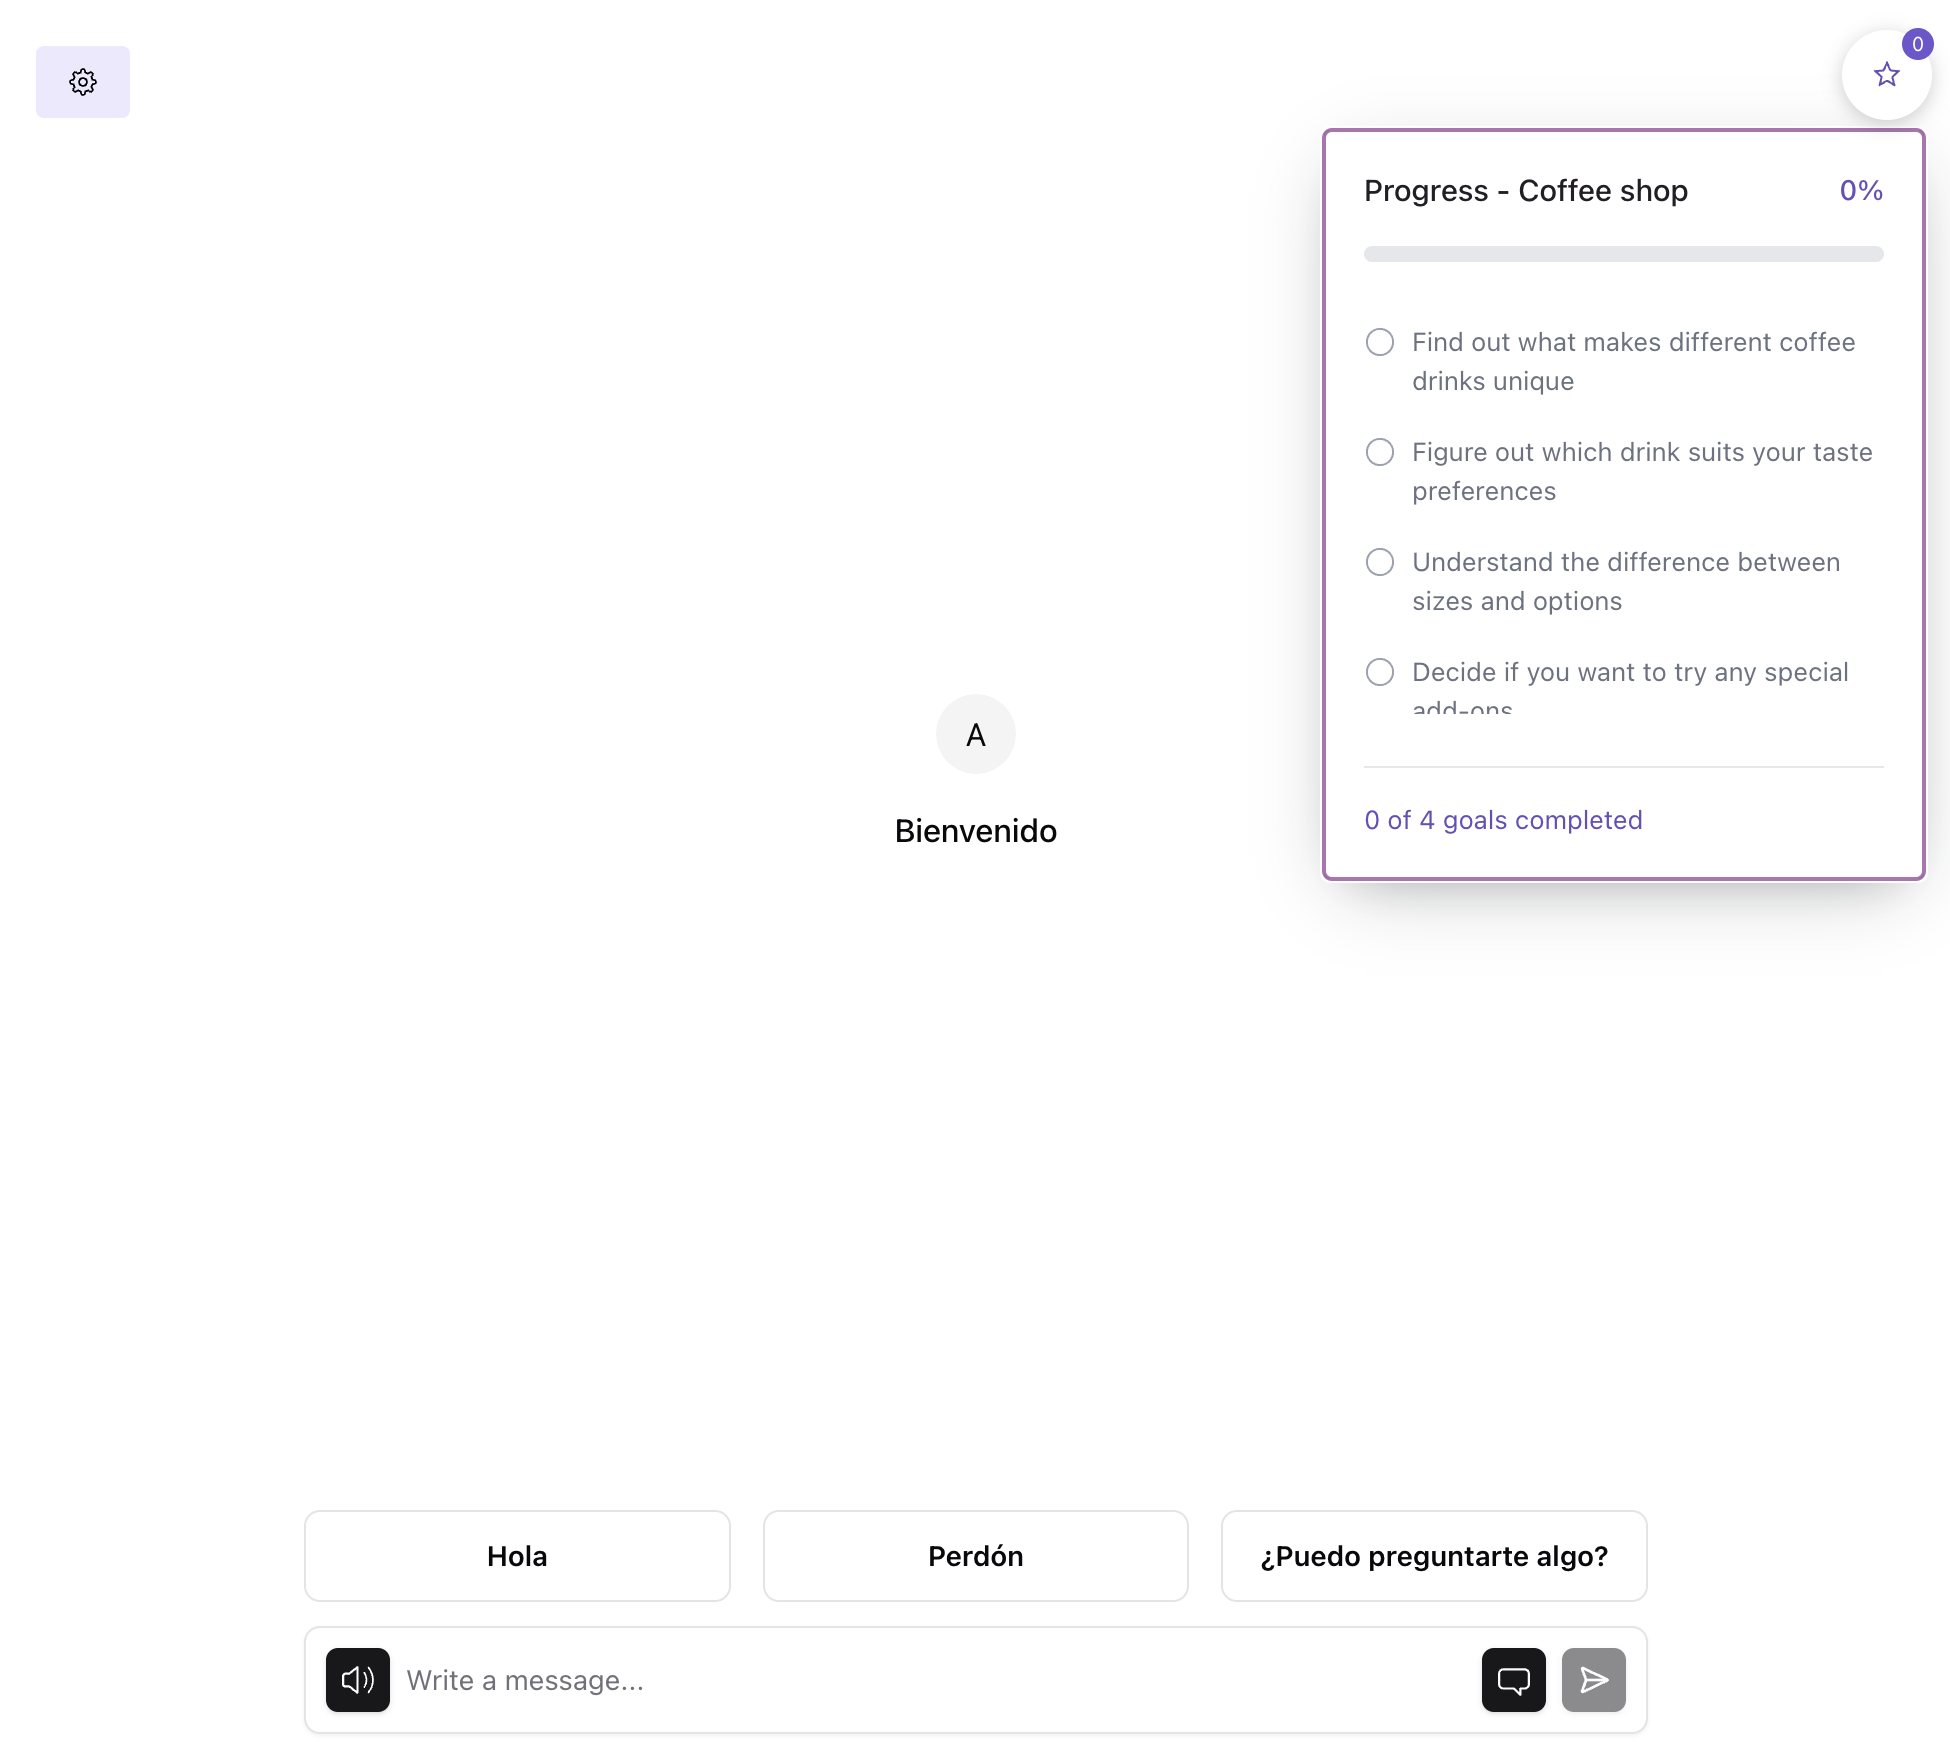
\includegraphics[width=0.8\textwidth]{figuras/screenshots/chat-initial.png}
    \caption{Interfaz principal del sistema mostrando el chat y las opciones de voz}
    \label{fig:main-interface}
\end{figure}


La Figura \ref{fig:main-interface} muestra la interfaz principal del sistema, diseñada siguiendo principios de simplicidad y accesibilidad. En esta interfaz se observan los siguientes elementos clave:

\begin{itemize}
    \item \textbf{Panel de chat interactivo:} Área central donde se desarrolla la conversación con el agente de aprendizaje, mostrando el historial de mensajes y permitiendo la entrada de texto.
    
    \item \textbf{Controles de voz:} Botones para activar las funcionalidades de \gls{tts} y \gls{stt}, permitiendo la práctica de comprensión y expresión oral.
    
    \item \textbf{Indicadores de nivel:} Visualización del nivel actual del estudiante según el marco \gls{cefr}, permitiendo al usuario comprender su progreso.
    
    \item \textbf{Menú de navegación:} Acceso a las diferentes secciones del sistema, incluyendo práctica, análisis y configuración.
\end{itemize}

\subsection{Sistema de Diálogo}
\label{subsec:sistema-dialogo}

\begin{figure}[H]
    \centering
    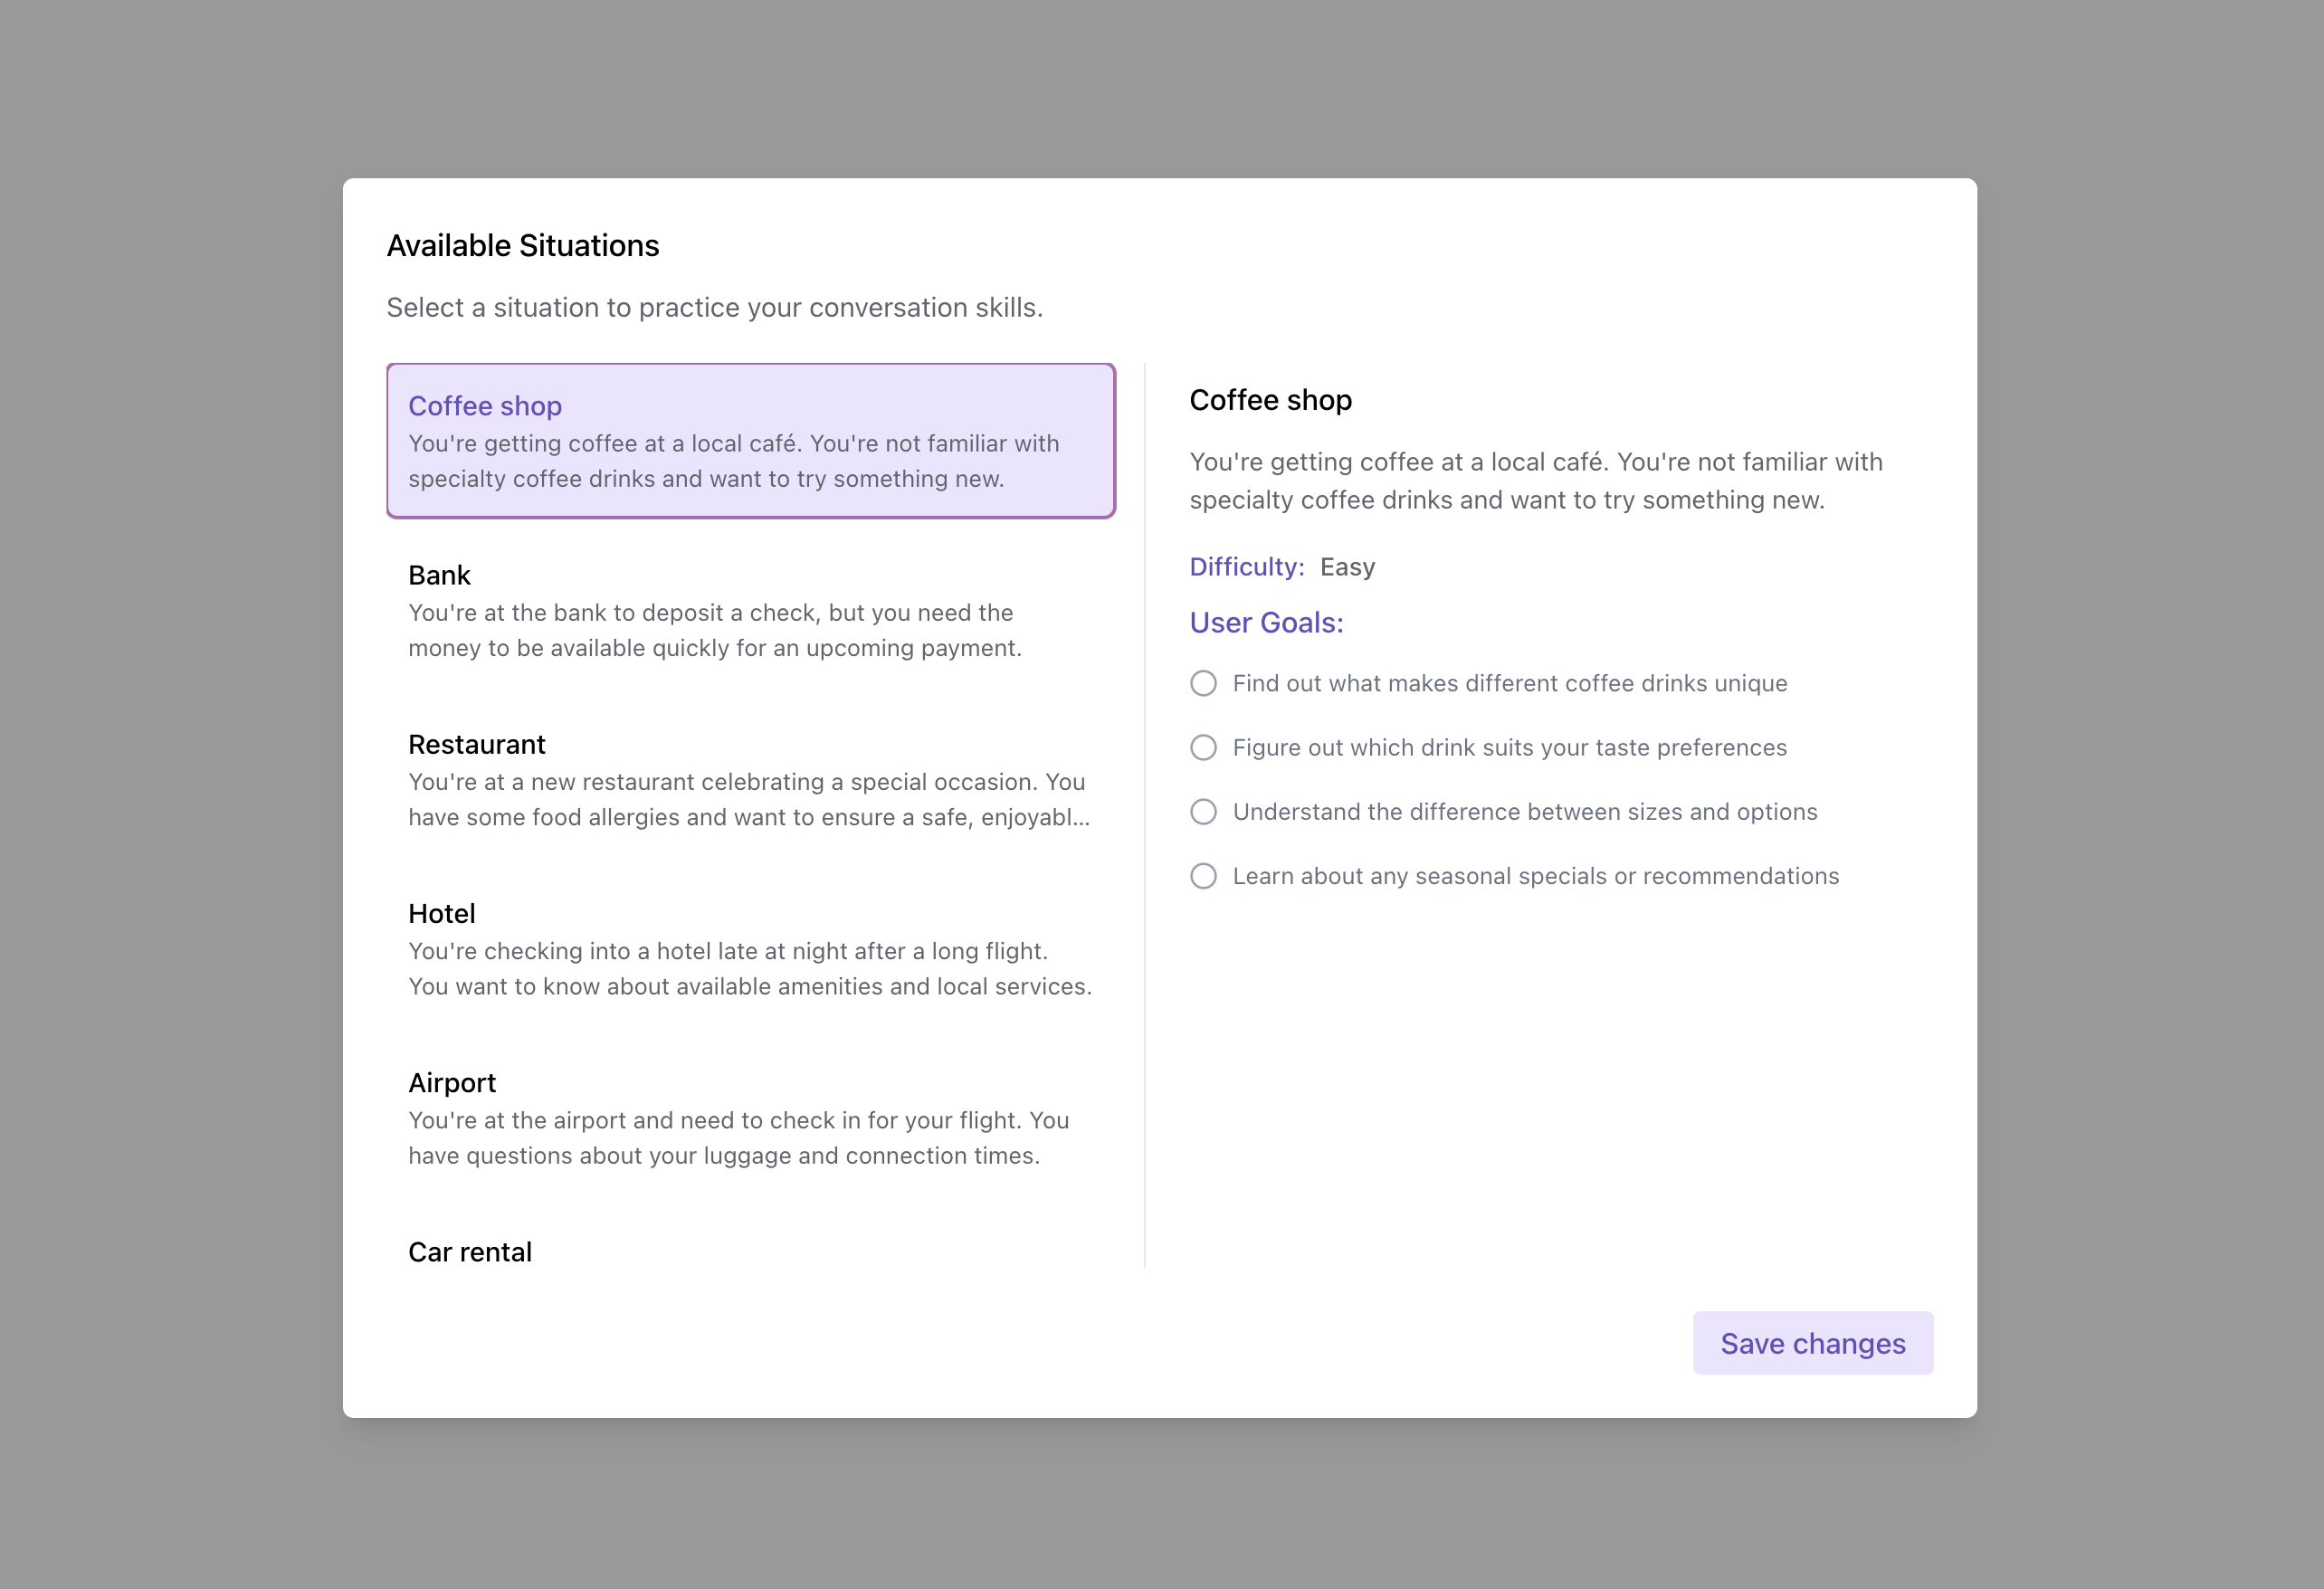
\includegraphics[width=0.8\textwidth]{figuras/screenshots/chat-complete.png}
    \caption{Sistema de diálogo mostrando una conversación de ejemplo}
    \label{fig:dialog-system}
\end{figure}

La Figura \ref{fig:dialog-system} ilustra el sistema de diálogo en funcionamiento, mostrando una conversación de ejemplo con el agente de aprendizaje. Los elementos destacables incluyen:

\begin{itemize}
    \item \textbf{Generación de respuestas contextuales:} El sistema proporciona respuestas adaptadas al contexto de la conversación y al nivel del estudiante, manteniendo coherencia temática y adecuación lingüística.
    
    \item \textbf{Integración de \gls{rag}:} Las respuestas se enriquecen con información recuperada de la base de conocimientos, proporcionando explicaciones precisas y ejemplos relevantes.
    
    \item \textbf{Sistema de corrección en tiempo real:} Feedback inmediato sobre errores gramaticales o léxicos, con explicaciones adaptadas al nivel del estudiante.
    
    \item \textbf{Indicadores de progreso:} Señales visuales que informan al estudiante sobre su avance en los objetivos de la conversación actual.
\end{itemize}

\subsection{Selector de Situaciones}
\label{selector-situaciones}

\begin{figure}[H]
    \centering
    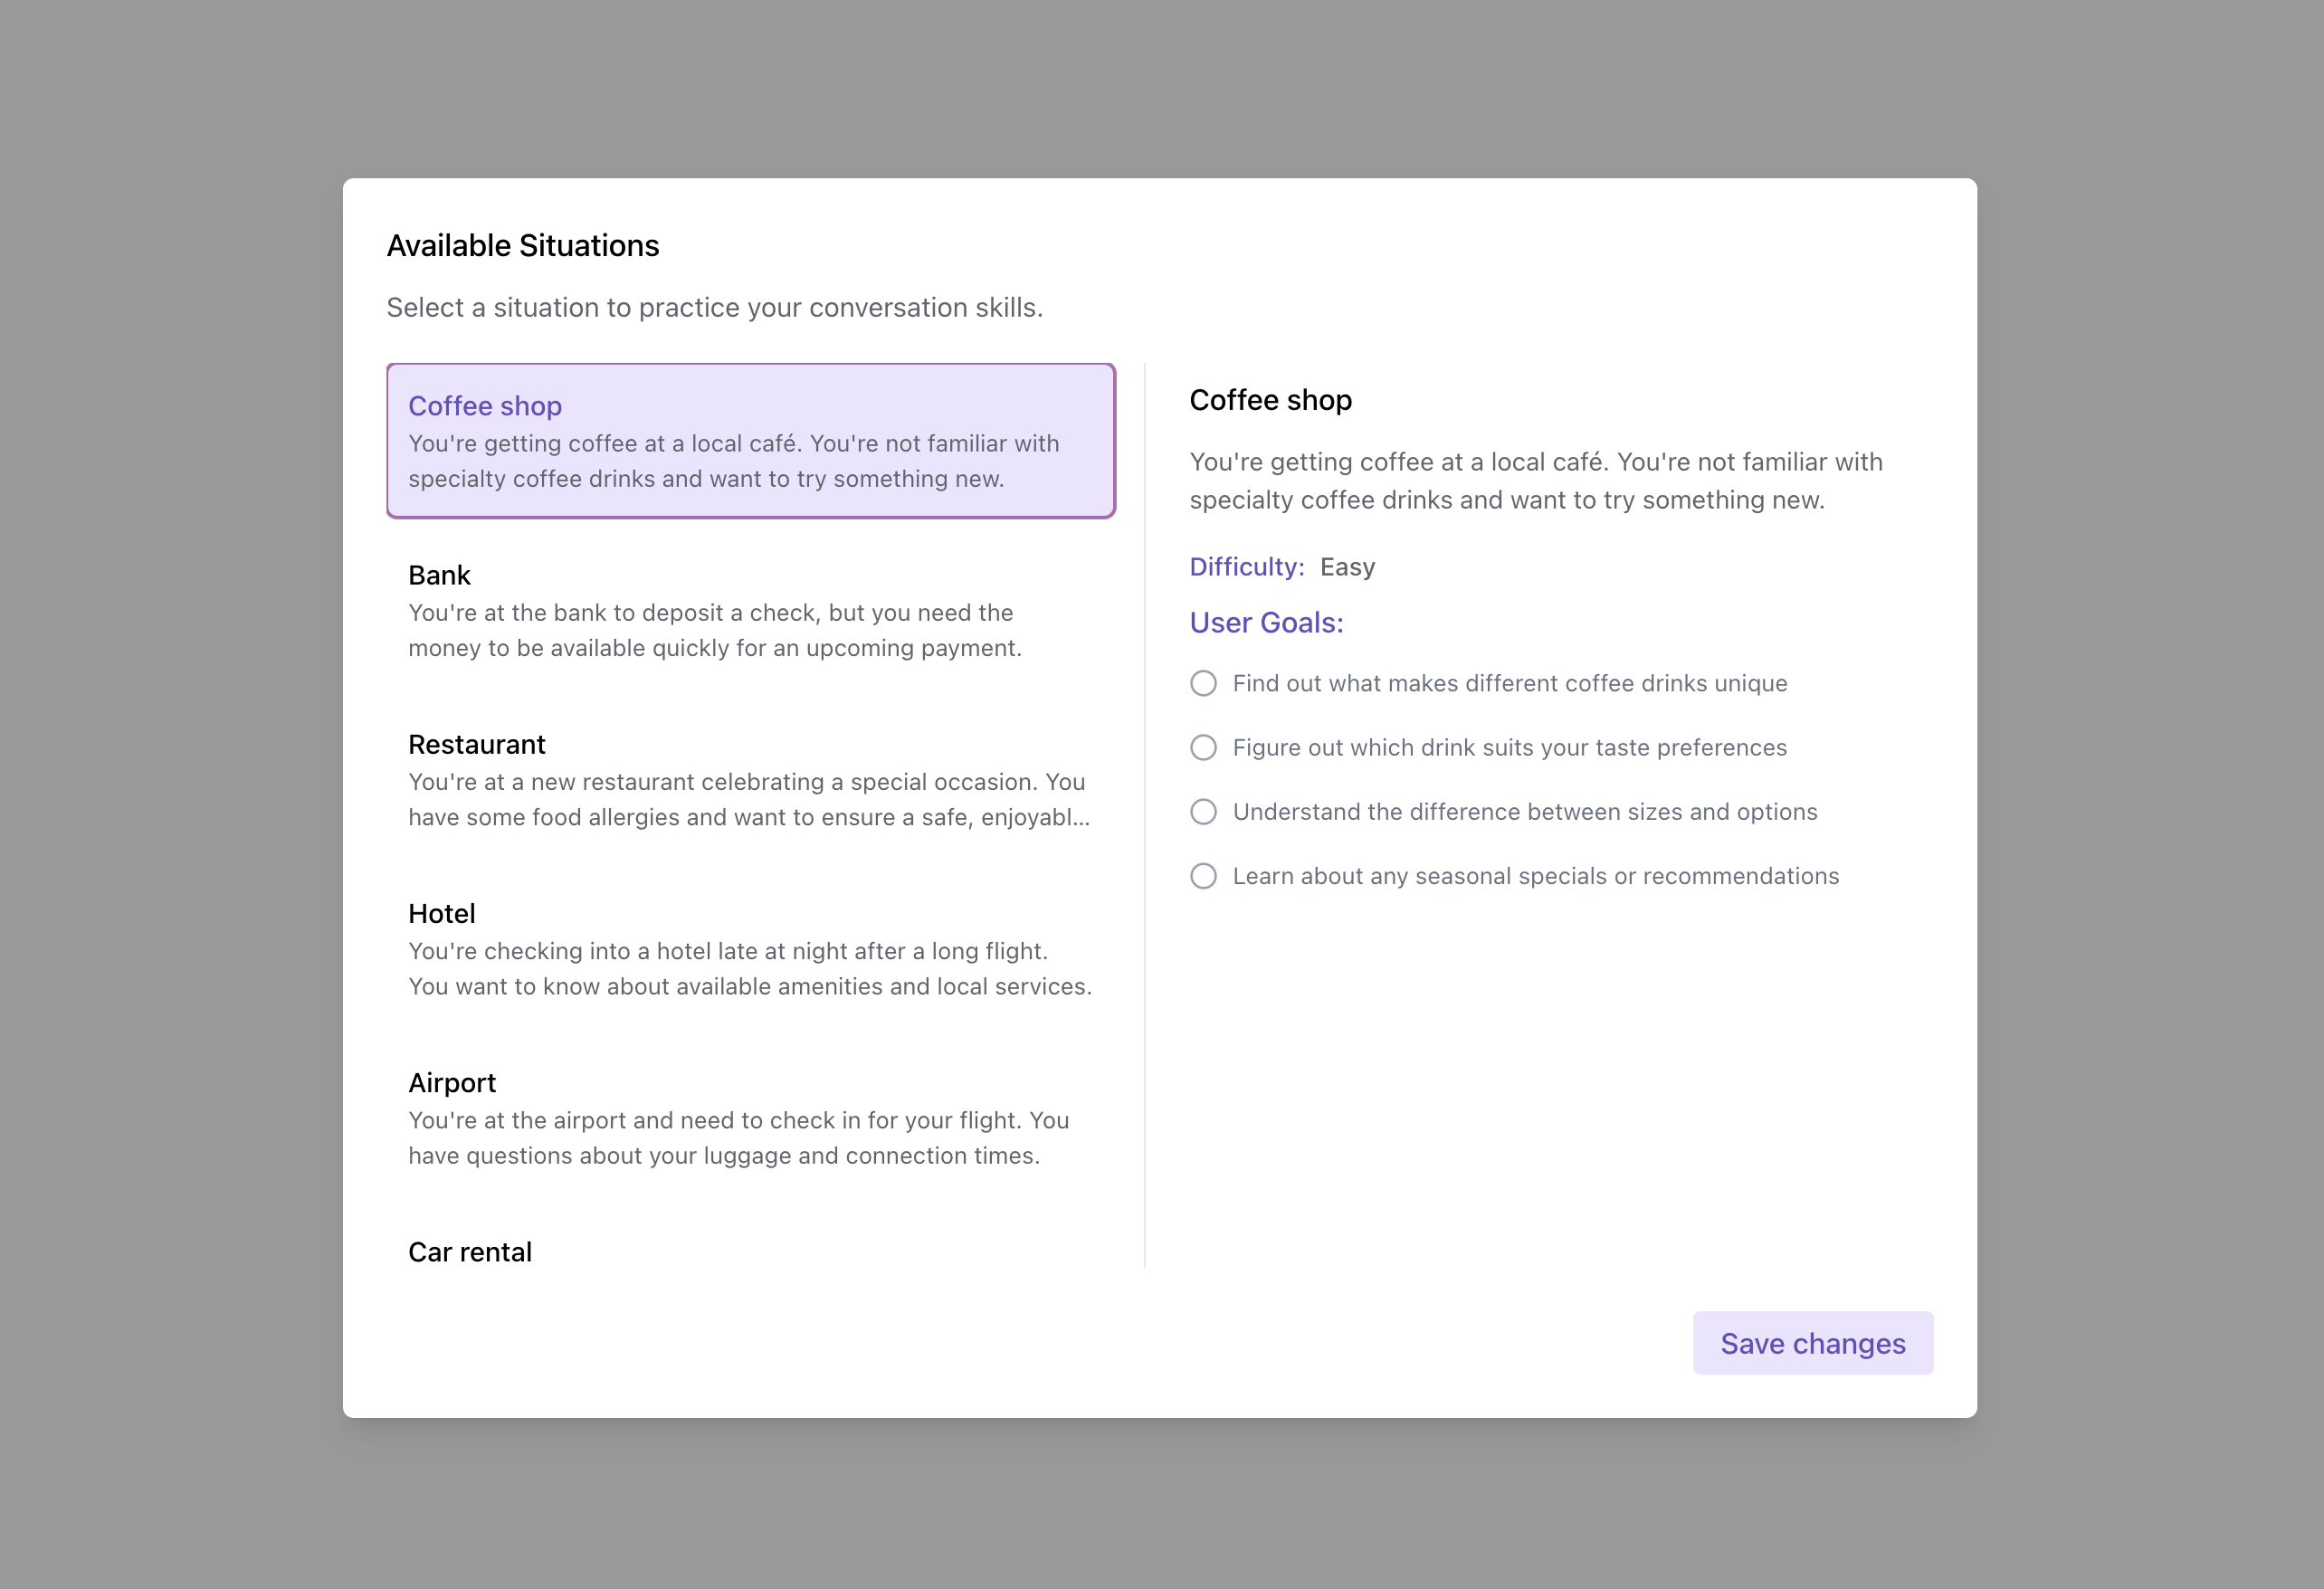
\includegraphics[width=0.8\textwidth]{figuras/screenshots/situation-picker.png}
    \caption{Interfaz de selección de contextos conversacionales y objetivos}
    \label{fig:situation-picker}
\end{figure}

La Figura \ref{fig:situation-picker} muestra la interfaz de selección de situaciones, un componente clave para la práctica contextualizada. Esta interfaz permite a los usuarios elegir escenarios específicos para su práctica conversacional, ofreciendo:

\begin{itemize}
    \item \textbf{Contextos Predefinidos:}
    \begin{itemize}
        \item Escenarios cotidianos como restaurantes, tiendas y oficinas
        \item Situaciones profesionales para entrevistas y reuniones
        \item Contextos académicos para estudiantes
        \item Situaciones sociales informales
    \end{itemize}
    
    \item \textbf{Sistema de Objetivos:}
    \begin{itemize}
        \item Lista clara de metas comunicativas a alcanzar durante la conversación
        \item Indicadores de progreso para cada objetivo específico
        \item Retroalimentación en tiempo real sobre el avance hacia las metas
    \end{itemize}
    
    \item \textbf{Personalización:}
    \begin{itemize}
        \item Adaptación automática del nivel de dificultad según el perfil del usuario
        \item Recomendaciones basadas en el historial de práctica y áreas de mejora
        \item Opciones para personalizar los objetivos específicos según necesidades
    \end{itemize}
\end{itemize}

\subsection{Panel de Análisis}
\label{panel-analisis}

\begin{figure}[H]
    \centering
    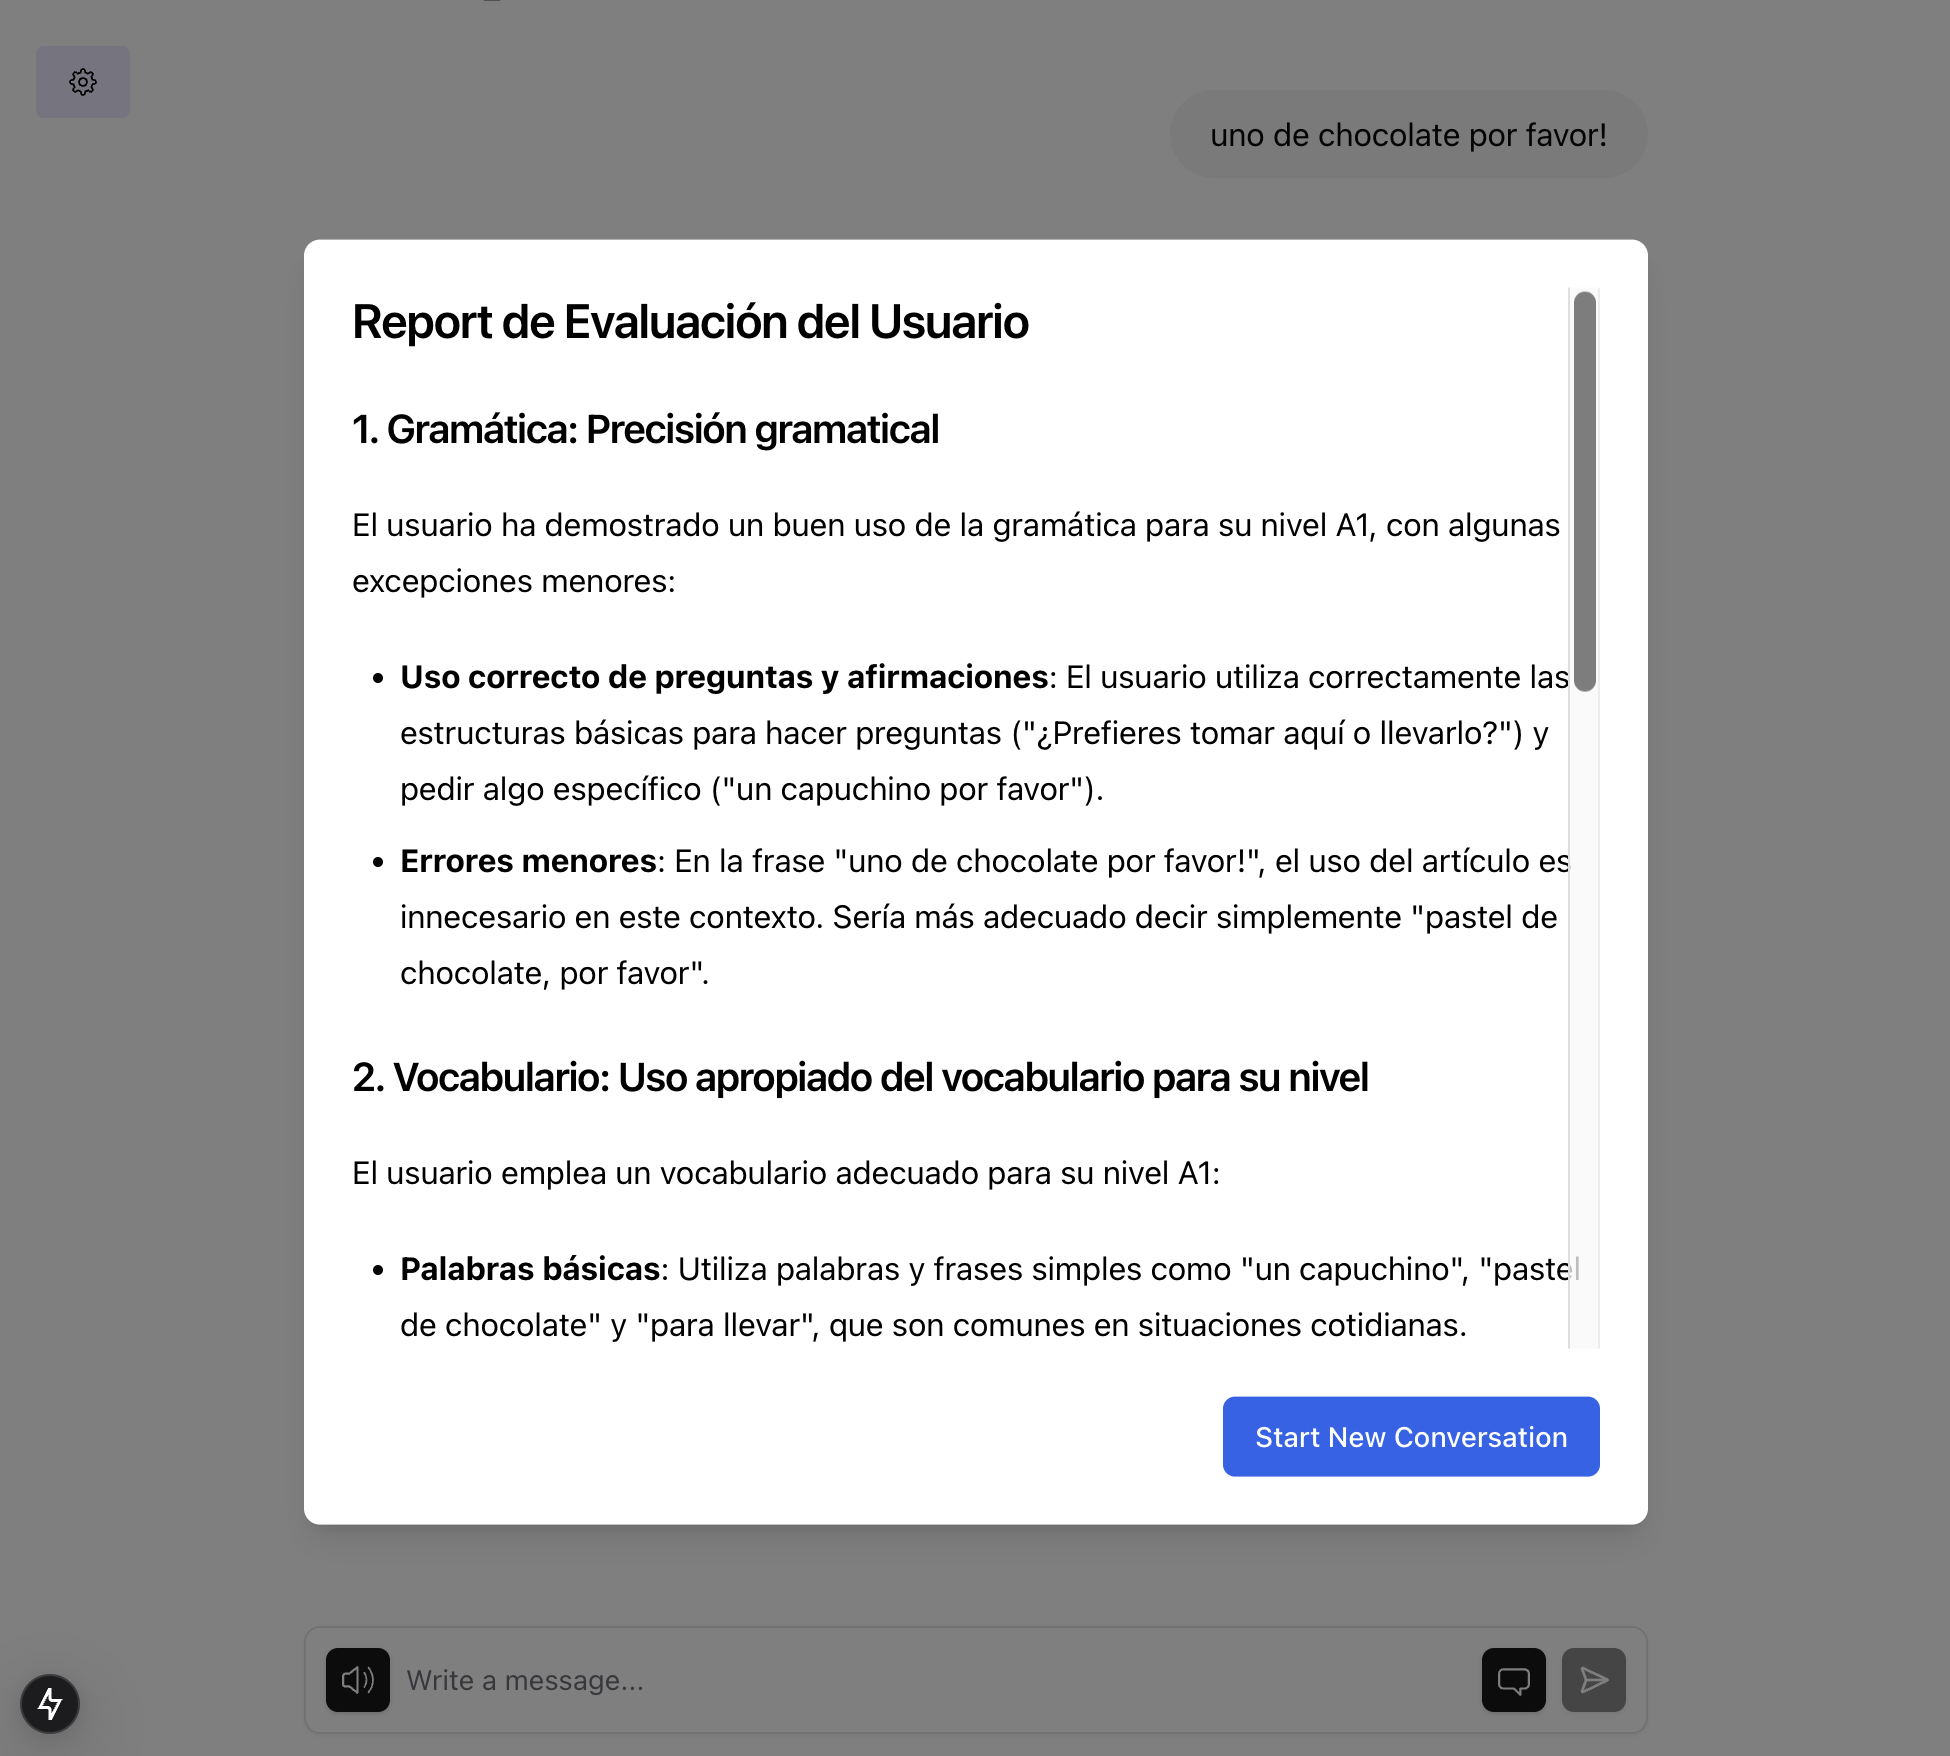
\includegraphics[width=0.8\textwidth]{figuras/screenshots/report.png}
    \caption{Panel de análisis mostrando métricas de aprendizaje}
    \label{fig:analytics-panel}
\end{figure}

La Figura \ref{fig:analytics-panel} muestra el panel de resultados, diseñado para proporcionar retroalimentación inmediata sobre el desempeño en la conversación. Este panel incluye:

\begin{itemize}
    \item \textbf{Objetivos cumplidos:} Registro de las metas alcanzadas durante la sesión de conversación.
    
    \item \textbf{Métricas de desempeño:} Evaluación de la conversación en tres dimensiones clave: gramática, vocabulario y fluidez, permitiendo al usuario identificar sus fortalezas y áreas de mejora.
    
    \item \textbf{Reporte personalizado:} Análisis detallado del desempeño con observaciones específicas sobre aspectos destacados y recomendaciones para mejorar.
    
    \item \textbf{Opciones de continuidad:} El usuario puede guardar su progreso y acceder posteriormente a la página de historial donde podrá visualizar su evolución a lo largo del tiempo.
\end{itemize}

\subsection{Visualización del Progreso de Aprendizaje}
\label{visualizacion-progreso}

\begin{figure}[H]
    \centering
    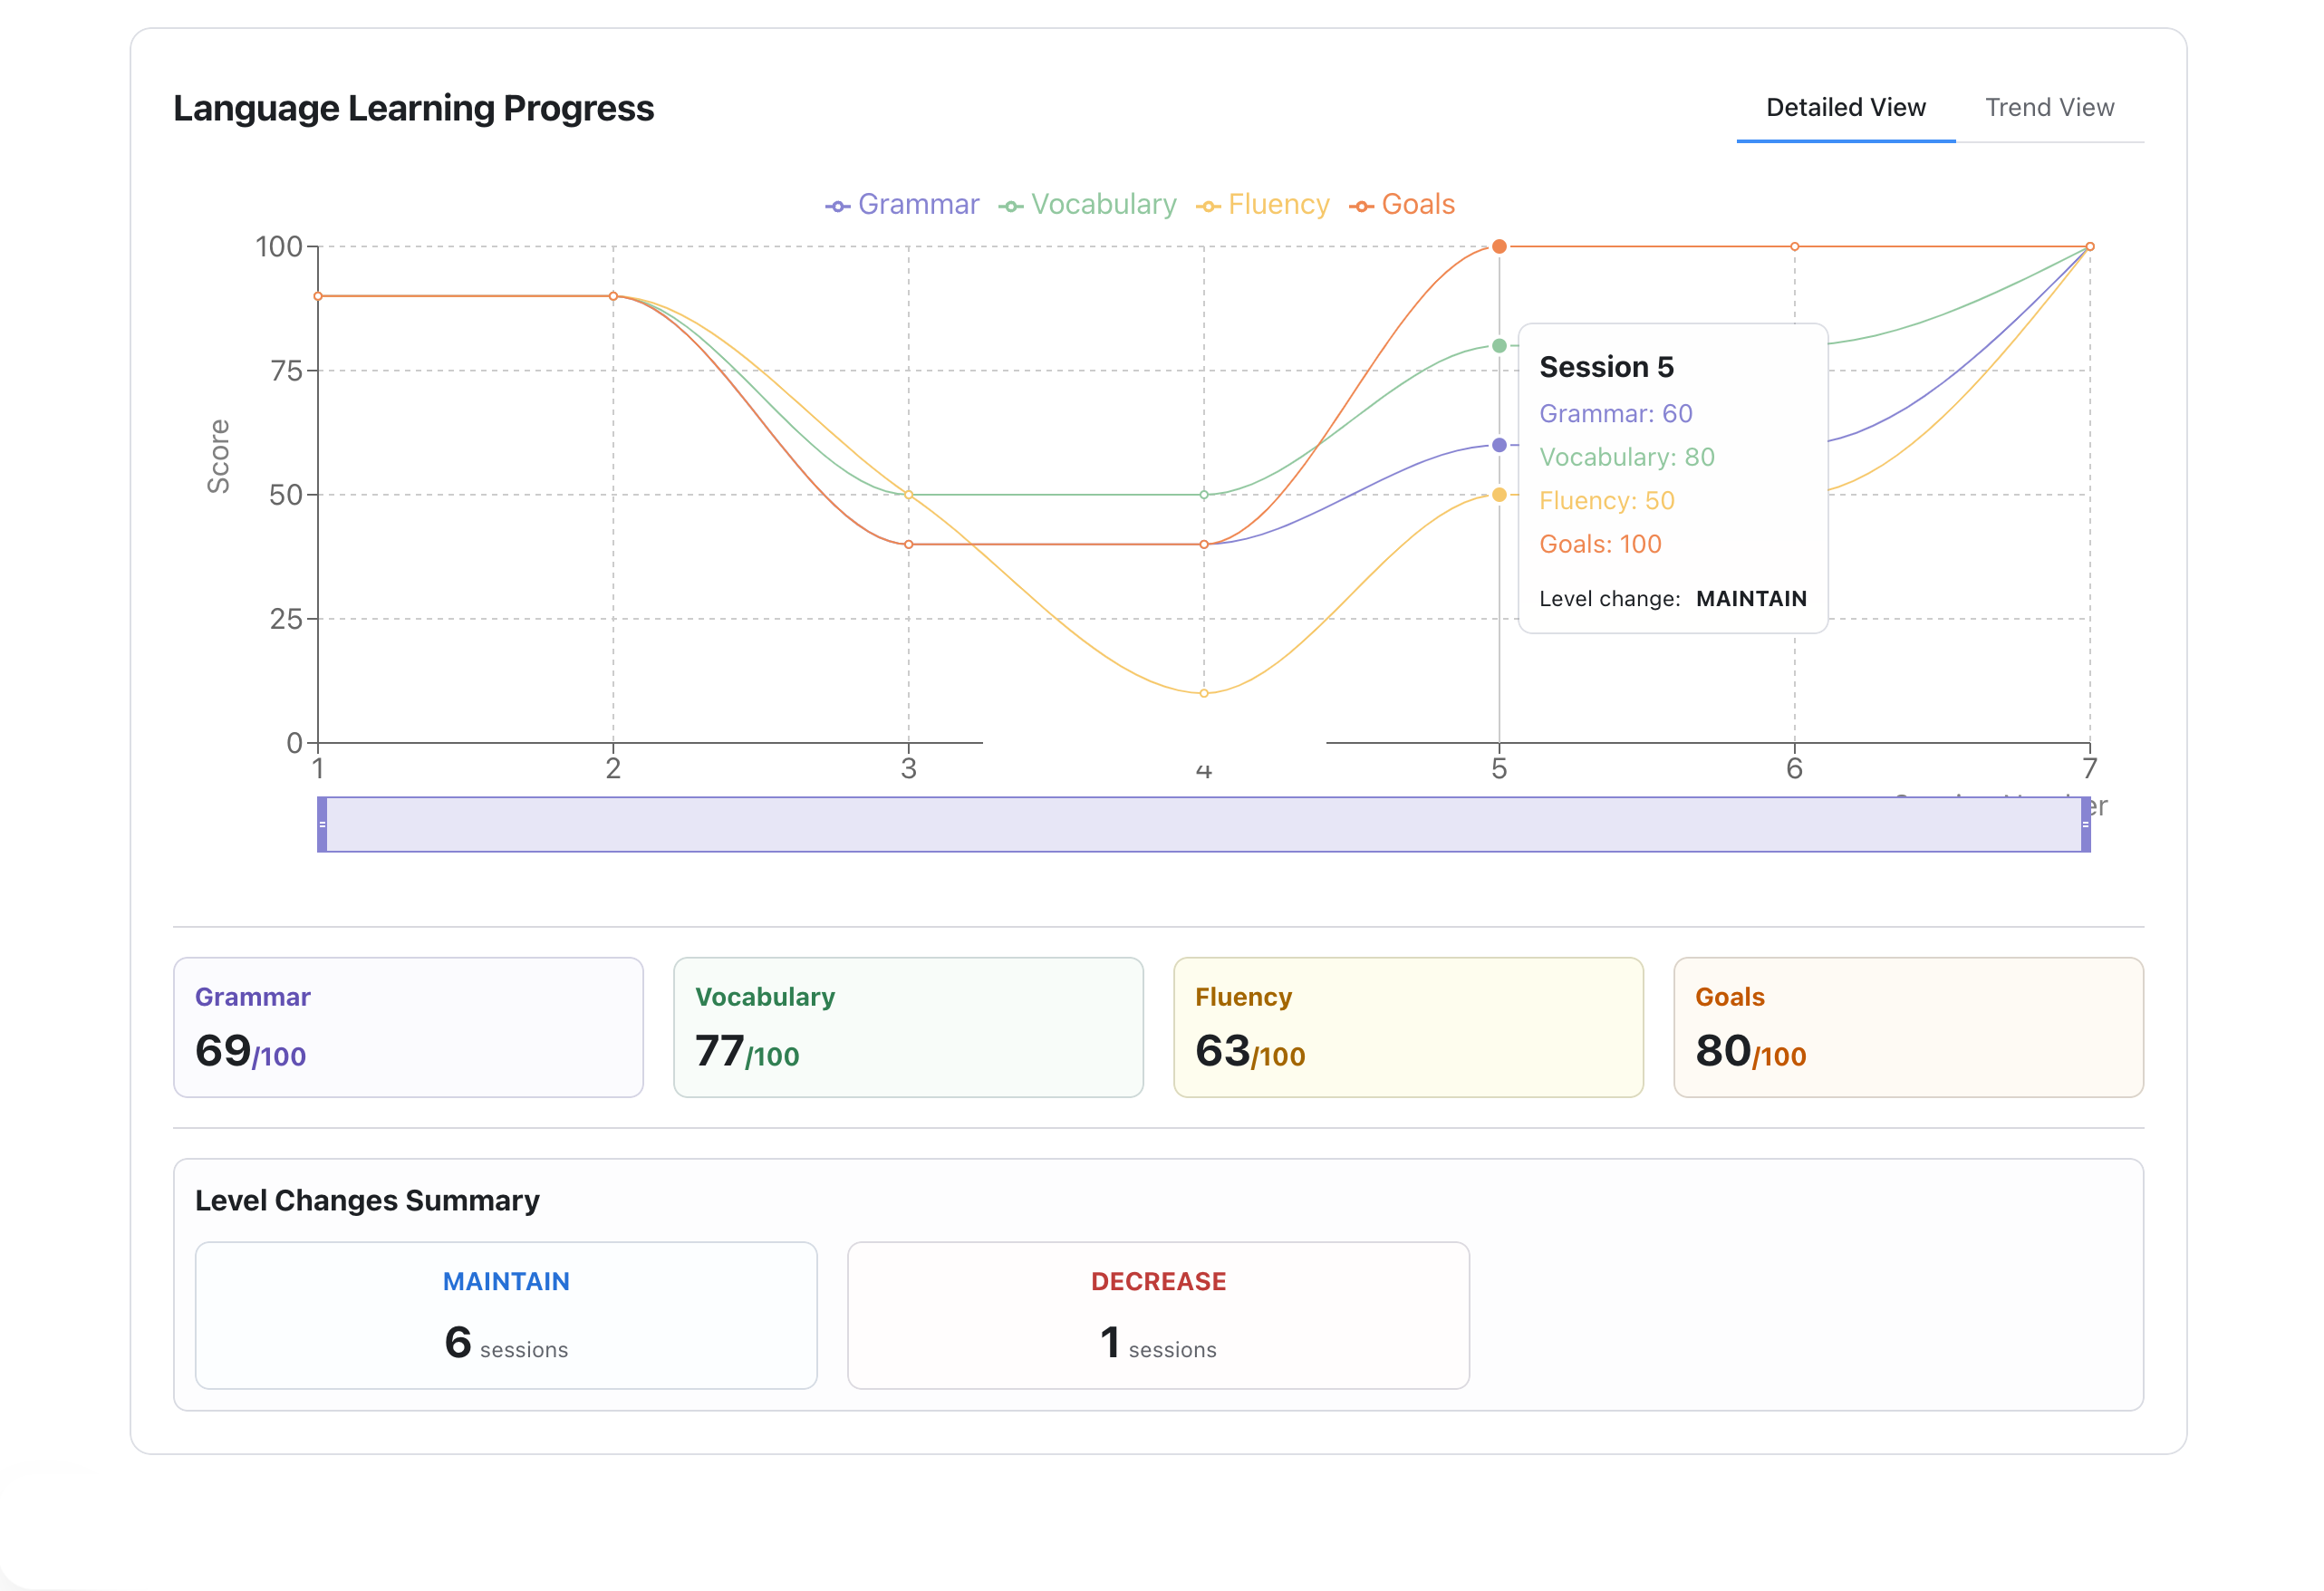
\includegraphics[width=0.8\textwidth]{figuras/screenshots/learning-history.png}
    \caption{Interfaz de visualización del progreso de aprendizaje con métricas detalladas}
    \label{fig:learning-history}
\end{figure}

La Figura \ref{fig:learning-history} muestra la interfaz de visualización del progreso de aprendizaje, un componente esencial para el seguimiento del desempeño del usuario. Esta herramienta proporciona una representación gráfica completa del desarrollo lingüístico a través de diversas funcionalidades integradas.

\begin{itemize}
    \item \textbf{Análisis Temporal Flexible:} Combina una vista detallada de sesiones individuales y una perspectiva de tendencias agrupadas, permitiendo al usuario alternar entre ambas modalidades para identificar tanto patrones generales como detalles específicos de su aprendizaje. El sistema incorpora controles interactivos que facilitan la exploración cronológica de los datos.
    
    \item \textbf{Evaluación Integral de Competencias Lingüísticas:} Monitoriza cuatro dimensiones fundamentales del aprendizaje: gramática, vocabulario, fluidez y cumplimiento de objetivos comunicativos. Cada métrica se presenta visualmente mediante un código de colores consistente que facilita la comparación entre habilidades y la identificación de fortalezas y áreas de mejora.
    
    \item \textbf{Análisis de Progresión de Nivel:} Ofrece un resumen visual de la trayectoria del aprendizaje, categorizando las sesiones según sus resultados (incremento, mantenimiento o descenso de nivel). Este componente proporciona contexto estadístico sobre el avance general, permitiendo correlacionar estrategias de práctica con resultados concretos.
    
    \item \textbf{Diseño Adaptativo y Accesible:} Implementado con Radix UI y técnicas responsivas para garantizar una experiencia óptima en cualquier dispositivo. La interfaz mantiene la integridad visual de los datos independientemente del tamaño de pantalla, priorizando la accesibilidad mediante contraste adecuado y elementos interactivos bien definidos.
\end{itemize}

Esta visualización del progreso constituye una herramienta fundamental para la reflexión metacognitiva del estudiante, permitiéndole identificar patrones en su aprendizaje y tomar decisiones informadas sobre sus futuras prácticas lingüísticas.

\section{Repositorios del Proyecto}
\label{sec:repositorios-proyecto}

El sistema ha sido desarrollado siguiendo una arquitectura cliente-servidor moderna, con separación clara entre la lógica de presentación y la de negocio. Todo el código fuente se encuentra disponible públicamente en GitHub bajo licencia MIT, promoviendo la transparencia, reproducibilidad y colaboración comunitaria.

\subsection{Estructura de Repositorios}
\label{subsec:estructura-repositorios}

\begin{itemize}
    \item \textbf{Frontend - Cliente:}
    \begin{itemize}
        \item Repositorio: \url{https://github.com/EmaSuriano/language-learning-client}
        \item Tecnologías: Next.js 14, TypeScript, Tailwind CSS
        \item Componentes principales:
              \begin{itemize}
                  \item Interfaz de chat basada en \gls{assistant-ui} con optimizaciones para aprendizaje
                  \item Selector de situaciones y objetivos con recomendaciones adaptativas
                  \item Gestión de estado con Zustand para manejo eficiente del contexto
                  \item Sistema de internacionalización con i18n (soporte para 8 idiomas)
                  \item Integración optimizada con API de audio para procesamiento de voz
              \end{itemize}
    \end{itemize}

    \item \textbf{Backend - Servidor:}
    \begin{itemize}
        \item Repositorio: \url{https://github.com/EmaSuriano/language-learning-server}
        \item Tecnologías: FastAPI, Python 3.10, LangChain, Stable-Baselines3
        \item Componentes principales:
              \begin{itemize}
                  \item Sistema \gls{rag} para recuperación contextual de recursos educativos
                  \item Integración con \gls{llm} (Phi-4) para generación de diálogos naturales
                  \item \gls{api-rest} con documentación OpenAPI para comunicación cliente-servidor
                  \item Implementación optimizada de Faster-Whisper y Kokoro-TTS
                  \item Sistema \gls{multi-agent} basado en LangChain para orquestación de agentes
                  \item Modelo \gls{ppo} implementado con Stable-Baselines3 para adaptación de nivel
              \end{itemize}
    \end{itemize}
\end{itemize}

\subsection{Documentación}
\label{subsec:documentacion-repositorios}

Ambos repositorios incluyen documentación exhaustiva para facilitar la comprensión, uso y extensión del sistema:

\begin{itemize}
    \item \textbf{Documentación General:}
    \begin{itemize}
        \item README principal con visión general del proyecto
        \item Guías de instalación detalladas para entornos de desarrollo y producción
        \item Diagramas de arquitectura y flujo de datos
        \item Guías de contribución para colaboradores externos
    \end{itemize}
    
    \item \textbf{Documentación Técnica:}
    \begin{itemize}
        \item Especificación completa de API mediante OpenAPI/Swagger
        \item Documentación de componentes y sus responsabilidades
        \item Variables de entorno requeridas con ejemplos y configuraciones recomendadas
        \item Guías de solución de problemas comunes
    \end{itemize}
    
    \item \textbf{Ejemplos y Tutoriales:}
    \begin{itemize}
        \item Ejemplos de uso para cada componente principal
        \item Tutoriales paso a paso para implementaciones personalizadas
        \item Guías para extensión de funcionalidades existentes
        \item Ejemplos de integración con sistemas externos
    \end{itemize}
\end{itemize}

Esta documentación exhaustiva facilita no solo la reproducibilidad de los resultados presentados, sino también la adaptación y extensión del sistema para diferentes contextos educativos y lingüísticos.

\section{Limitaciones Actuales y Trabajo Futuro}
\label{sec:limitaciones-trabajo-futuro}

A pesar de los resultados prometedores obtenidos, es importante reconocer las limitaciones actuales del sistema y definir las líneas de trabajo futuro para abordarlas.

\subsection{Limitaciones Identificadas}
\label{subsec:limitaciones-identificadas}

\begin{itemize}
    \item \textbf{Limitaciones Técnicas:}
    \begin{itemize}
        \item Precisión del sistema \gls{stt} insuficiente para acentos no nativos fuertes
        \item Tiempo de carga inicial del sistema relativamente alto (5-8 segundos)
        \item Dependencia de conexión a internet para funcionalidades avanzadas
        \item Consumo de recursos computacionales significativo para dispositivos de gama baja
    \end{itemize}

    \item \textbf{Limitaciones Pedagógicas:}
    \begin{itemize}
        \item Cobertura limitada de situaciones específicas de dominio (técnico, legal, médico)
        \item Sistema de evaluación aún no validado con metodologías educativas formales
        \item Adaptación insuficiente a diferentes estilos de aprendizaje
        \item Ausencia de mecanismos para aprendizaje colaborativo entre estudiantes
    \end{itemize}

    \item \textbf{Limitaciones de Validación:}
    \begin{itemize}
        \item Muestra reducida en pruebas preliminares (n=10)
        \item Período de evaluación relativamente corto (2 semanas)
        \item Ausencia de grupo de control para comparación con métodos tradicionales
        \item Falta de evaluación longitudinal del impacto en el aprendizaje
    \end{itemize}
\end{itemize}


\subsection{Trabajo Futuro}

En base a las limitaciones identificadas y los resultados preliminares, se plantean las siguientes líneas de trabajo futuro:

\begin{itemize}
    \item \textbf{Evaluación Exhaustiva:}
    \begin{itemize}
        \item Diseño de estudio con muestra ampliada (n>100) y diversificada geográficamente
        \item Implementación de evaluación longitudinal (3-6 meses) para medir impacto real
        \item Desarrollo de metodología comparativa con grupo de control usando métodos tradicionales
        \item Validación con profesionales de la enseñanza de idiomas y expertos en pedagogía
    \end{itemize}

    \item \textbf{Mejoras Técnicas:}
    \begin{itemize}
        \item Refinamiento del modelo \gls{ppo} mediante fine-tuning con datos reales de usuarios
        \item Adaptación específica del sistema \gls{stt} para mejorar precisión con acentos no nativos
        \item Optimización de la base de conocimientos del \gls{rag} con expansión temática y actualización automática
        \item Implementación de modos offline para funcionalidades básicas sin conexión
    \end{itemize}

    \item \textbf{Expansión de Funcionalidades:}
    \begin{itemize}
        \item Desarrollo de módulos específicos para dominios especializados (negocios, turismo, academia)
        \item Implementación de componente social para práctica colaborativa entre estudiantes
        \item Integración con contenido auténtico (noticias, videos, podcasts) para inmersión contextual
        \item Desarrollo de sistema de gamificación adaptativa para aumentar motivación y retención
    \end{itemize}
\end{itemize}

Estas líneas de trabajo futuro representan un plan estructurado para abordar las limitaciones actuales y expandir las capacidades del sistema, con el objetivo de maximizar su impacto educativo y mejorar la experiencia de aprendizaje para una gama más amplia de usuarios.

Los resultados presentados en este capítulo, aunque preliminares, proporcionan evidencia inicial sobre la viabilidad y potencial del enfoque propuesto. En el siguiente capítulo, se discutirán las conclusiones generales del trabajo, analizando las contribuciones realizadas, las lecciones aprendidas durante el desarrollo, y las implicaciones más amplias de estos avances para el futuro del aprendizaje de idiomas asistido por tecnología.
\chapter{Conclusiones}
\label{conclusiones}


\cleardoublepage
\phantomsection

% Appendix
\appendix
\chapter{Anexo: Faster Whisper y Modelos de Transcripción}
\label{anexo-faster-whisper}

Este anexo explora Faster Whisper, una implementación optimizada del modelo Whisper de OpenAI para transcripción y traducción de voz a texto. Se analizan sus características principales, arquitectura, y se compara el rendimiento entre los diferentes modelos disponibles.

\section{Características Principales}
\label{sec:faster-whisper-features}

Faster Whisper representa una mejora significativa sobre la implementación original de Whisper, destacando por:

\begin{itemize}
	\item \textbf{Optimización CTranslate2}: Utiliza el toolkit CTranslate2 para optimizar la inferencia del modelo.
	\item \textbf{Menor Consumo de Memoria}: Reduce significativamente el uso de memoria mediante técnicas de cuantización.
	\item \textbf{Aceleración por Hardware}: Aprovecha eficientemente CPU y GPU mediante paralelización.
	\item \textbf{Detección de Voz}: Integra VAD (Voice Activity Detection) para mejorar la precisión.
\end{itemize}

\section{Arquitectura del Sistema}
\label{sec:faster-whisper-architecture}

\begin{figure}[H]
	\caption{Arquitectura de Faster Whisper}
	\label{fig:whisper}
	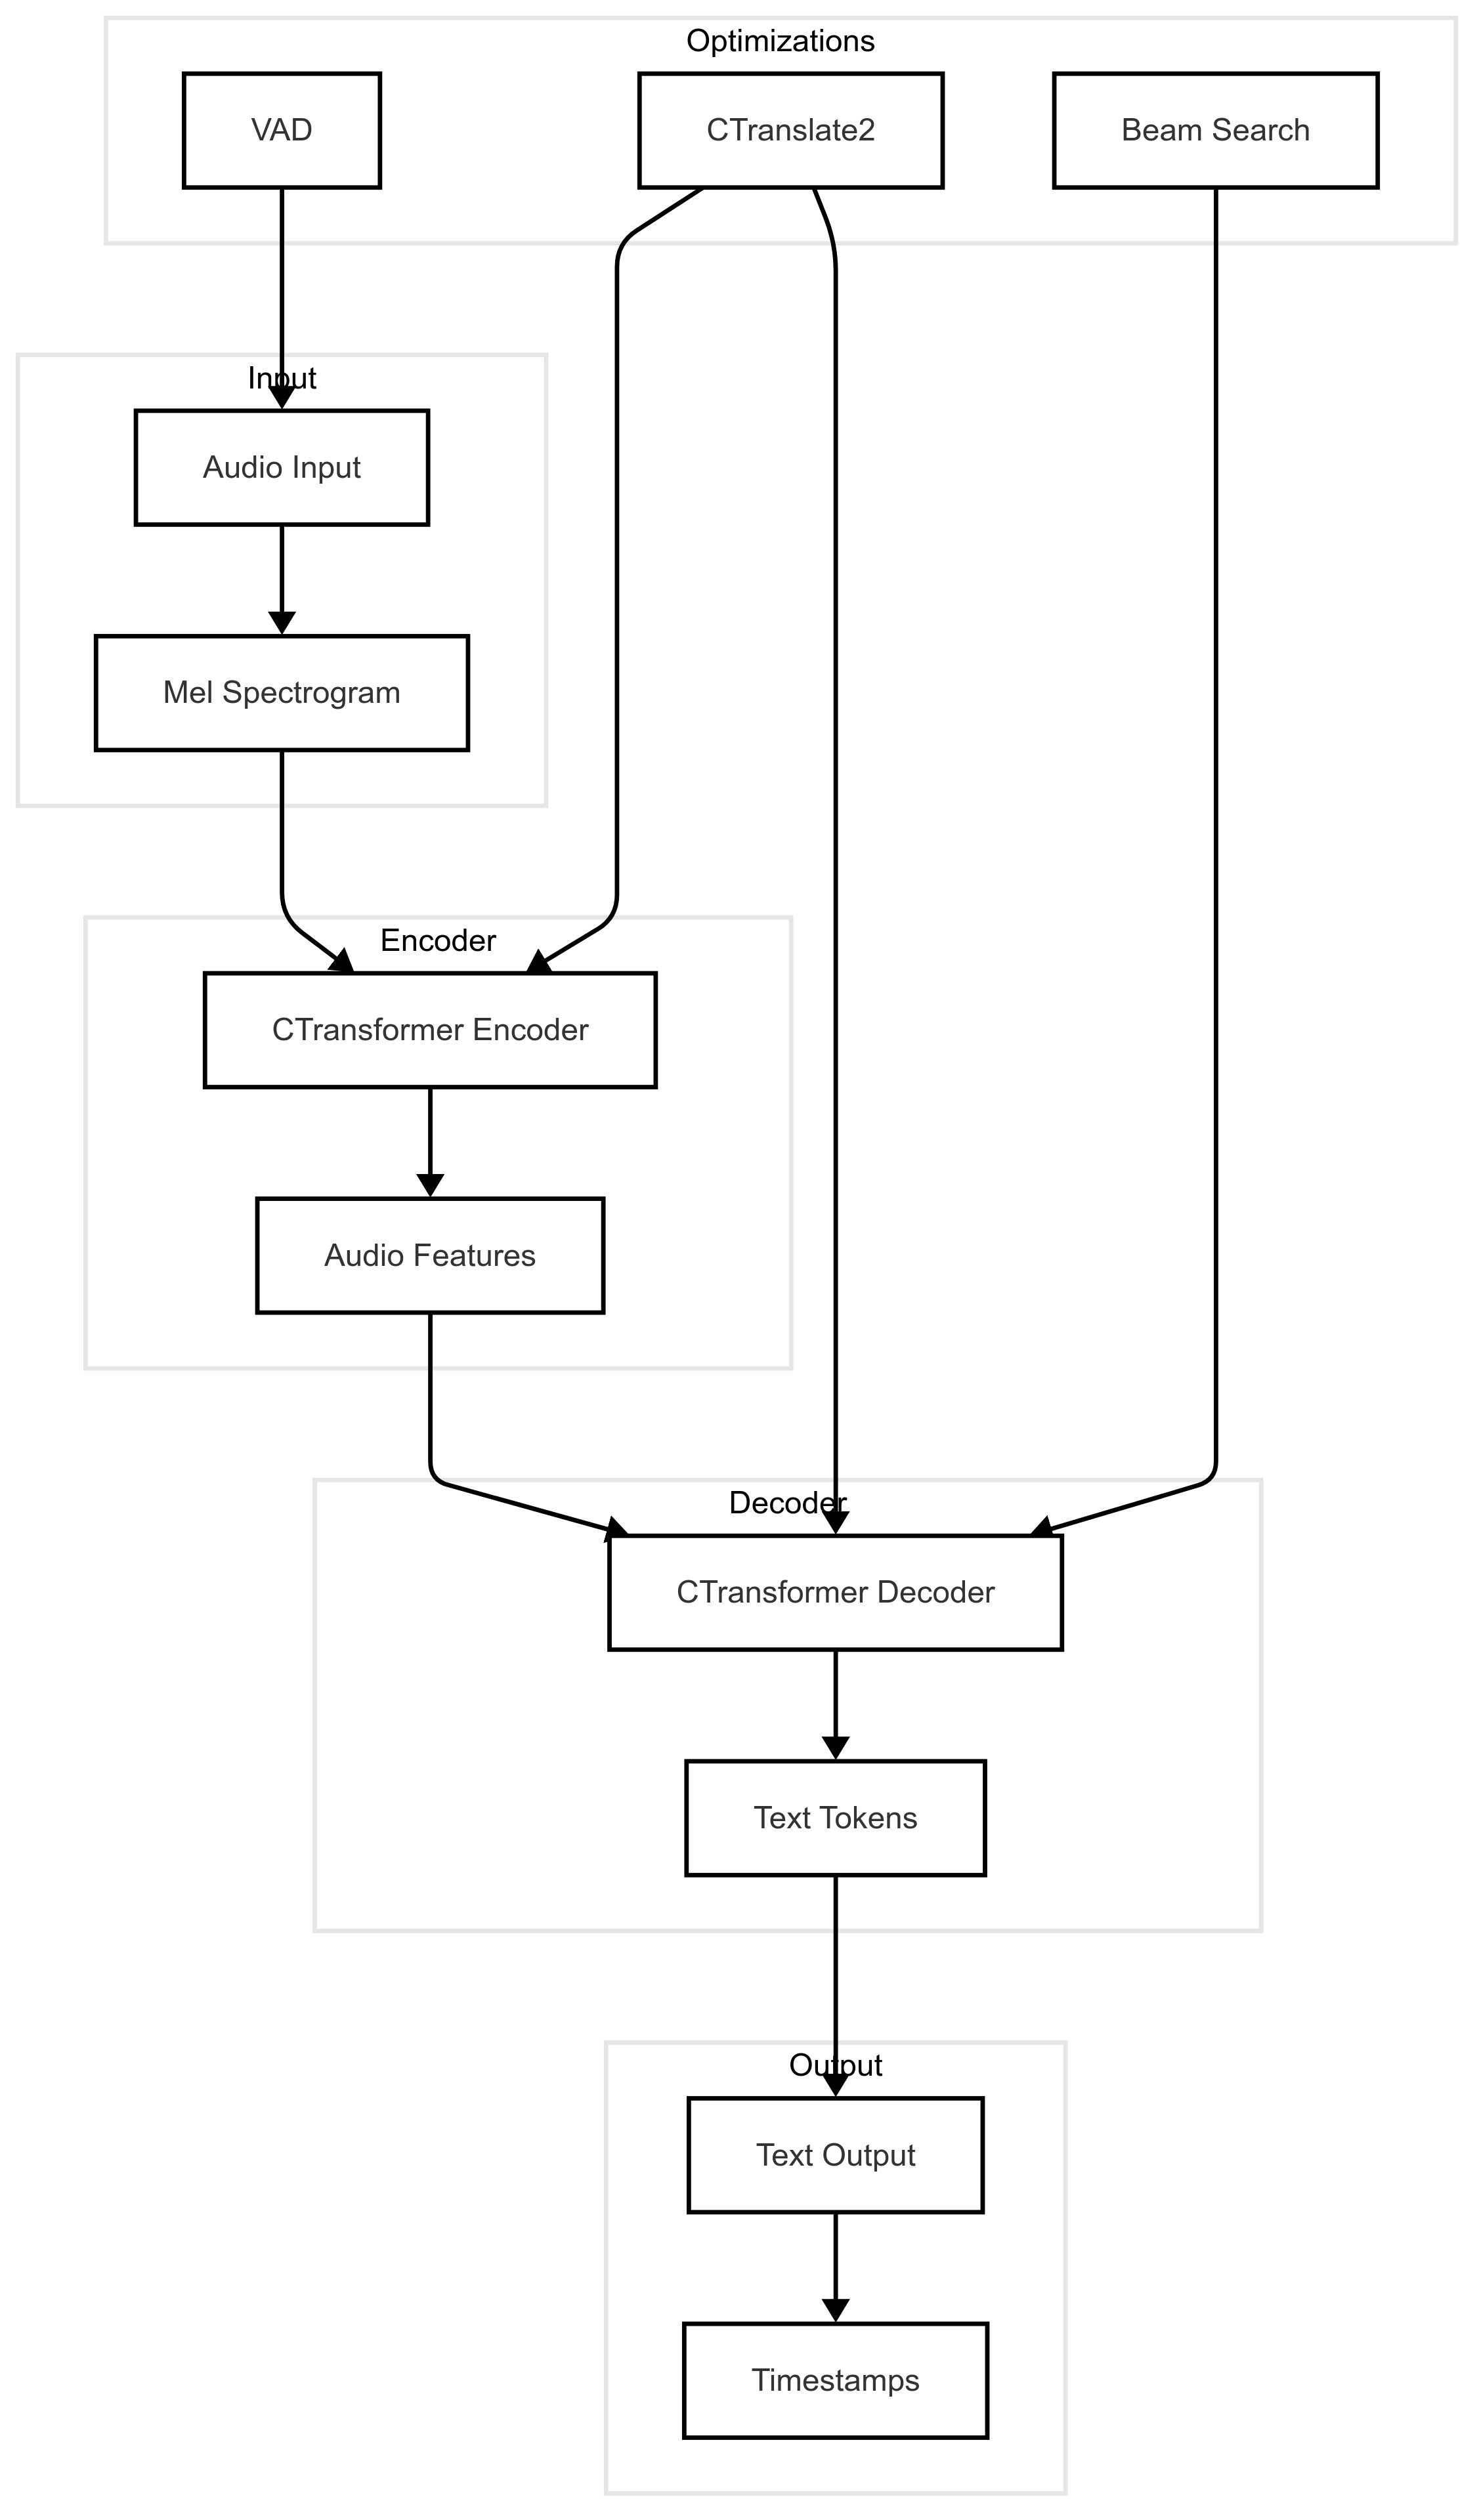
\includegraphics[width=0.8\textwidth]{figuras/whisper.png}
\end{figure}

La arquitectura de Faster Whisper se compone de varios módulos especializados que trabajan en conjunto para proporcionar transcripción eficiente:

\subsection{Componentes Principales}
\label{subsec:main-components}

\subsubsection{Preprocesamiento de Audio}
El sistema procesa la entrada de audio mediante:
\begin{equation}
	\text{mel} = \text{log}(\max(\text{STFT}(x), \epsilon))
\end{equation}
donde STFT es la Transformada de Fourier de Tiempo Corto y $\epsilon$ es un valor pequeño para estabilidad numérica.

\subsubsection{CTransformer}
La implementación utiliza CTranslate2 para optimizar:
\begin{itemize}
	\item \textbf{Encoder}: Procesa el espectrograma mel en representaciones de audio.
	\item \textbf{Decoder}: Genera tokens de texto mediante atención cruzada.
\end{itemize}

\section{Comparativa de Modelos Whisper}
\label{sec:whisper-models-comparison}

\begin{table}[H]
	\caption{Comparación de modelos Whisper}
	\label{tab:whisper-models}
	\begin{tabular}{|p{2cm}|p{2cm}|p{3cm}|p{3cm}|p{3cm}|}
		\hline
		\textbf{Modelo} & \textbf{Parámetros} & \textbf{RAM (FP16)} & \textbf{WER} & \textbf{Velocidad Relativa} \\
		\hline
		Tiny            & 39M                 & 1GB                 & 7.1\%        & 32x                         \\
		\hline
		Base            & 74M                 & 1.5GB               & 6.1\%        & 16x                         \\
		\hline
		Small           & 244M                & 2.5GB               & 5.2\%        & 8x                          \\
		\hline
		Medium          & 769M                & 4.5GB               & 4.3\%        & 4x                          \\
		\hline
		Large           & 1550M               & 7.5GB               & 3.6\%        & 1x                          \\
		\hline
	\end{tabular}
\end{table}

\subsection{Características por Modelo}
\label{subsec:model-features}

\begin{itemize}
	\item \textbf{Tiny}:
	      \begin{itemize}
		      \item Ideal para dispositivos con recursos limitados
		      \item Mejor opción para transcripción en tiempo real
		      \item Rendimiento aceptable en condiciones de audio limpias
	      \end{itemize}

	\item \textbf{Base}:
	      \begin{itemize}
		      \item Balance entre rendimiento y recursos
		      \item Adecuado para aplicaciones web
		      \item Buen rendimiento en múltiples idiomas
	      \end{itemize}

	\item \textbf{Small}:
	      \begin{itemize}
		      \item Mejora significativa en precisión sobre Base
		      \item Soporte robusto para múltiples acentos
		      \item Detección confiable de cambios de idioma
	      \end{itemize}

	\item \textbf{Medium}:
	      \begin{itemize}
		      \item Alta precisión en condiciones desafiantes
		      \item Excelente rendimiento en audio con ruido
		      \item Capacidad avanzada de puntuación
	      \end{itemize}

	\item \textbf{Large}:
	      \begin{itemize}
		      \item Máxima precisión disponible
		      \item Mejor rendimiento en audios complejos
		      \item Capacidad superior de traducción
	      \end{itemize}
\end{itemize}

\section{Optimizaciones}
\label{sec:optimizations}

\subsection{Técnicas de Cuantización}
\label{subsec:quantization}

Faster Whisper implementa varias técnicas de cuantización:

\begin{itemize}
	\item \textbf{INT8}: Reduce el tamaño del modelo en 4x con mínima pérdida de precisión
	\item \textbf{INT16}: Balance entre precisión y tamaño
	\item \textbf{FLOAT16}: Máxima precisión con reducción de memoria
\end{itemize}

\subsection{Paralelización}
\label{subsec:parallelization}

El sistema implementa múltiples niveles de paralelización:

\begin{itemize}
	\item \textbf{Batch Processing}: Procesa múltiples segmentos simultáneamente
	\item \textbf{Thread Pooling}: Optimiza la utilización de CPU
	\item \textbf{GPU Acceleration}: Aprovecha CUDA para procesamiento paralelo
\end{itemize}

\section{Consideraciones de Implementación}
\label{sec:implementation-considerations}

\subsection{Selección de Modelo}
La elección del modelo debe considerar:

\begin{itemize}
	\item \textbf{Recursos Disponibles}: Memoria y capacidad de procesamiento
	\item \textbf{Requisitos de Latencia}: Tiempo de respuesta necesario
	\item \textbf{Precisión Requerida}: Tolerancia a errores
\end{itemize}

\subsection{Estrategias de Deployment}
Consideraciones para el despliegue:

\begin{itemize}
	\item \textbf{Edge Computing}: Procesamiento en dispositivo para menor latencia
	\item \textbf{Server-Side}: Mayor capacidad de procesamiento pero mayor latencia
	\item \textbf{Hybrid}: Combinación según necesidades específicas
\end{itemize}

\chapter{Anexo: Kokoro TTS}
\label{anexo-kokoro}

Este anexo explora Kokoro TTS, un modelo de síntesis de voz de código abierto que destaca por su eficiencia y calidad comparable a modelos más grandes, a pesar de contar con solo 82 millones de parámetros. El modelo implementa una arquitectura ligera basada en StyleTTS 2 e ISTFTNet, diseñada para ofrecer una síntesis de voz de alta calidad con recursos computacionales limitados.

\section{Arquitectura del Sistema}
\label{sec:kokoro-architecture}

La arquitectura de Kokoro TTS se fundamenta en dos componentes principales: StyleTTS 2 e ISTFTNet. Esta combinación permite una síntesis de voz eficiente mientras mantiene una alta calidad en la salida.

\subsection{Componentes Principales}
\label{subsec:main-components}

\begin{itemize}
	\item \textbf{Misaki G2P}: Sistema de conversión de grafemas a fonemas que soporta múltiples idiomas.
	\item \textbf{Style Encoder}: Codifica las características de estilo de voz a partir de audio de referencia.
	\item \textbf{Decoder}: Genera características acústicas basadas en los fonemas y el estilo.
	\item \textbf{ISTFT Network}: Realiza la síntesis final del audio mediante transformada inversa de Fourier.
\end{itemize}

\section{Características Técnicas}
\label{sec:technical-features}

\subsection{Especificaciones del Modelo}
\begin{itemize}
	\item \textbf{Parámetros}: 82 millones
	\item \textbf{Arquitectura Base}: StyleTTS 2 + ISTFTNet
	\item \textbf{Licencia}: Apache 2.0
	\item \textbf{Formato de Audio}: 24kHz, mono
\end{itemize}

\subsection{Conjunto de Datos}
El entrenamiento se realizó exclusivamente con datos de audio permitidos:
\begin{itemize}
	\item Audio de dominio público
	\item Audio con licencias permisivas (Apache, MIT)
	\item Audio sintético de modelos comerciales
\end{itemize}

\section{Análisis de Voces}
\label{sec:voice-analysis}

\subsection{Sistema de Calificación}
\label{subsec:grading-system}

El sistema evalúa las voces mediante dos métricas principales:

\begin{itemize}
	\item \textbf{Calidad Objetivo}:
	      \begin{itemize}
		      \item A: Calidad excepcional
		      \item B: Buena calidad
		      \item C: Calidad aceptable
		      \item D: Calidad limitada
	      \end{itemize}

	\item \textbf{Duración del Entrenamiento}:
	      \begin{itemize}
		      \item HH: 10-100 horas
		      \item H: 1-10 horas
		      \item MM: 10-100 minutos
		      \item M: 1-10 minutos
	      \end{itemize}
\end{itemize}

\subsection{Distribución de Voces}
\label{subsec:voice-distribution}

\begin{table}[H]
	\centering
	\caption{Distribución y calidad de voces por idioma}
	\label{tab:voice-distribution}
	\begin{tabular}{|l|c|c|c|l|}
		\hline
		\textbf{Idioma}  & \textbf{F} & \textbf{M} & \textbf{Total} & \textbf{Calidad Media} \\
		\hline
		Inglés Americano & 11         & 9          & 20             & B-                     \\
		\hline
		Inglés Británico & 4          & 4          & 8              & C+                     \\
		\hline
		Japonés          & 4          & 1          & 5              & C+                     \\
		\hline
		Chino Mandarín   & 4          & 4          & 8              & D+                     \\
		\hline
		Español          & 1          & 2          & 3              & C                      \\
		\hline
		Francés          & 1          & 0          & 1              & B-                     \\
		\hline
		Hindi            & 2          & 2          & 4              & C                      \\
		\hline
		Italiano         & 1          & 1          & 2              & C                      \\
		\hline
		Portugués BR     & 1          & 2          & 3              & C                      \\
		\hline
	\end{tabular}
\end{table}

\section{Rendimiento y Limitaciones}
\label{sec:performance}

\subsection{Rangos Óptimos de Operación}
\label{subsec:optimal-ranges}

El rendimiento del modelo varía según la longitud del texto:
\begin{itemize}
	\item \textbf{Rango Óptimo}: 100-200 tokens
	\item \textbf{Rendimiento Reducido}: <20 tokens
	\item \textbf{Posible Aceleración}: >400 tokens
\end{itemize}

\subsection{Costos de Entrenamiento}
\label{subsec:training-costs}

El entrenamiento de Kokoro ha sido notablemente eficiente:
\begin{itemize}
	\item \textbf{Horas GPU}: 1000 horas en A100 80GB
	\item \textbf{Costo Total}: Aproximadamente \$1000 USD
	\item \textbf{Tasa Promedio}: \$1/hora
\end{itemize}

\section{Comparativa con Otros Modelos}
\label{sec:model-comparison}

\begin{table}[H]
	\centering
	\caption{Comparación con modelos TTS similares}
	\label{tab:model-comparison}
	\begin{tabular}{|l|c|c|c|c|}
		\hline
		\textbf{Modelo} & \textbf{Parámetros} & \textbf{Voces} & \textbf{Idiomas} & \textbf{Licencia} \\
		\hline
		Kokoro          & 82M                 & 54             & 8                & Apache            \\
		\hline
		Coqui           & 1000M               & 1087           & 100+             & MIT               \\
		\hline
		Bark            & 900M                & 100+           & 100+             & MIT               \\
		\hline
	\end{tabular}
\end{table}

% Bibliography
\begin{singlespace}
  \begin{footnotesize}
    \begin{twocolumn}
      \bibliography{bibliografia}
      \addcontentsline{toc}{chapter}{Bibliografía}
    \end{twocolumn}
  \end{footnotesize}
\end{singlespace}

\end{document}